
\documentclass[5p]{elsarticle}


\usepackage[table]{xcolor}
\usepackage{lmodern}

\usepackage[utf8]{inputenc}
\usepackage[T1]{fontenc}
\usepackage{url}

\usepackage{xspace}
\newcommand{\ie}[0]{{\em i.e.},\xspace}
\newcommand{\vs}[0]{{\em vs.}\xspace}
\newcommand{\eg}[0]{{\em e.g.},\xspace}
\newcommand{\etal}[0]{{\em et al.}\xspace}
\newcommand{\wrt}[0]{{\em w.r.t.}\xspace}
\newcommand{\aka}[0]{{\em a.k.a.}\xspace}
\newcommand{\via}[0]{{\em via}\xspace}

\newcommand{\ecotype}[0]{\emph{nantes-ecotype}\xspace}
\newcommand{\nova}[0]{\emph{lyon-nova}\xspace}

\newcommand{\ansass}[0]{\emph{m\_ansible}\xspace}
\newcommand{\aeoass}[0]{\emph{m\_aeolus}\xspace}
\newcommand{\madass}[0]{\emph{madeus}\xspace}

\newcommand{\shell}[0]{\textsc{Shell}\xspace}
\newcommand{\fractal}[0]{\textsc{Fractal}\xspace}
\newcommand{\bash}[0]{\emph{bash}\xspace}
\newcommand{\ruby}[0]{\textsc{Ruby}\xspace}
\newcommand{\ansible}[0]{\textsc{Ansible}\xspace}
\newcommand{\chef}[0]{\textsc{Chef}\xspace}
\newcommand{\puppet}[0]{\textsc{Puppet}\xspace}
\newcommand{\salt}[0]{\textsc{Salt}\xspace}
\newcommand{\cfengine}[0]{\textsc{CFEngine}\xspace}
\newcommand{\deployware}[0]{\textsc{DeployWare}\xspace}
\newcommand{\juju}[0]{\textsc{Juju}\xspace}
\newcommand{\kubernetes}[0]{\textsc{Kubernetes}\xspace}
\newcommand{\terraform}[0]{\textsc{Terraform}\xspace}
\newcommand{\aeolus}[0]{\textsc{Aeolus}\xspace}
\newcommand{\mad}[0]{\textsc{Madeus}\xspace}
\newcommand{\cloudformation}[0]{\textsc{CloudFormation}\xspace}
\newcommand{\heat}[0]{\textsc{Heat}\xspace}
\newcommand{\tosca}[0]{\textsc{Tosca}\xspace}
\newcommand{\dockerswarm}[0]{\textsc{Docker Swarm}\xspace}
\newcommand{\nix}[0]{\textsc{Nix}\xspace}
\newcommand{\docker}[0]{\textsc{Docker}\xspace}
\newcommand{\kolla}[0]{Kolla\xspace}
\newcommand{\apache}[0]{\textsc{Apache}\xspace}
\newcommand{\mysql}[0]{\textsc{MySQL}\xspace}
\newcommand{\implem}[0]{PoC\xspace}
\newcommand{\llc}{L\textsuperscript{2}C\xspace}
\newcommand{\net}[0]{\emph{internal-net}\xspace}

\usepackage{caption}

\usepackage[colorlinks]{hyperref}
\usepackage{url}

\usepackage[textwidth=17mm]{todonotes}
\newcommand{\customtodo}[4]{
        \todo[color=#2,inline,size=\small]{
                \ifx&#3&
                        \textbf{#1} #4
                \else
                        \textbf{#1$\Rightarrow$#3} #4
                \fi
        }
}
\newcommand{\MC}[2][]{\customtodo{MC}{red!50}{#1}{#2}}
\newcommand{\HC}[2][]{\customtodo{HC}{red!20}{#1}{#2}}
\newcommand{\CP}[2][]{\customtodo{CP}{blue!20}{#1}{#2}}
\newcommand{\DP}[2][]{\customtodo{DP}{blue!50}{#1}{#2}}
\newcommand{\CS}[2][]{\customtodo{CS}{green!20}{#1}{#2}}
\newcommand{\SR}[2][]{\customtodo{SR}{green!20}{#1}{#2}}
\usepackage{amsmath,amssymb,amsfonts}
\usepackage{mathtools}
\usepackage{subfig}
\usepackage[export]{adjustbox}
\usepackage{pifont}
\usepackage{wasysym}

\usepackage{booktabs} % For formal tables
\usepackage{array,multirow}
\newcommand{\STAB}[1]{\begin{tabular}{@{}c@{}}#1\end{tabular}}

\usepackage{siunitx}
\usepackage{cleveref}

\usepackage{tikz}
\usetikzlibrary{shapes.geometric, arrows}
\tikzstyle{place} = [rectangle, rounded corners, minimum width=2cm, minimum height=1cm,text centered, draw=black, fill=red!40]
\tikzstyle{leaving} = [rectangle, rounded corners, minimum width=2cm, minimum height=1cm,text centered, draw=black, fill=red!20]
\tikzstyle{provide_start} = [rectangle, rounded corners, minimum width=2cm, minimum height=1cm,text centered, draw=black, fill=orange!40]
\tikzstyle{provide_stop} = [rectangle, rounded corners, minimum width=2cm, minimum height=1cm,text centered, draw=black, fill=blue!20]
\tikzstyle{use_start} = [rectangle, rounded corners, minimum width=2cm, minimum height=1cm,text centered, draw=black, fill=orange!20]
\tikzstyle{use_stop} = [rectangle, rounded corners, minimum width=2cm, minimum height=1cm,text centered, draw=black, fill=blue!40]
\tikzstyle{end} = [rectangle, rounded corners, minimum width=2cm, minimum height=1cm,text centered, draw=black, fill=gray!20]
\tikzstyle{beginning} = [rectangle, rounded corners, minimum width=2cm, minimum height=1cm,text centered, draw=black, fill=gray!40]
\tikzstyle{control} = [rectangle, rounded corners, minimum width=2cm, minimum height=1cm,text centered, draw=black, fill=orange!30]
\tikzstyle{arrow} = [thick,->,>=stealth]

\def\cmark{\tikz\fill[scale=0.4](0,.35) -- (.25,0) -- (1,.7) -- (.25,.15) -- cycle;}

% lstlisting python + colors
\usepackage{color}
\usepackage[procnames]{listings}
\definecolor{keywords}{RGB}{255,0,90}
\definecolor{comments}{RGB}{0,0,113}
\definecolor{red}{RGB}{160,0,0}
\definecolor{green}{RGB}{0,150,0}
\definecolor{backcolour}{rgb}{0.95,0.95,0.95}
\DeclareCaptionFont{white}{\color{white}}
\DeclareCaptionFont{gray}{\color{gray}}
\DeclareCaptionFormat{listing}{\colorbox{gray}{\parbox{\linewidth}{#1#2#3}}}
\captionsetup[lstlisting]{format=listing,labelfont=white,textfont=white}
\lstset{language=Python,
        numbers=left,
        backgroundcolor=\color{backcolour},
        numbersep=5pt,
        keywordstyle=\color{keywords},
        commentstyle=\color{comments},
        stringstyle=\color{red},
        showstringspaces=false,
        identifierstyle=\color{green},
        procnamekeys={def,class},
        basicstyle=\scriptsize\ttfamily,
        numberstyle=\tiny\color{gray},
%       frame=single
}

% Fix for bibliography
\makeatletter
\providecommand{\doi}[1]{%
  \begingroup
    \let\bibinfo\@secondoftwo
    \urlstyle{rm}%
    \href{http://dx.doi.org/#1}{%
      doi:\discretionary{}{}{}%
      \nolinkurl{#1}%
    }%
  \endgroup
}
\makeatother

\usepackage{amsthm}
\newtheorem{theorem}{Theorem}[subsection]
\newtheorem{lemma}{Lemma}[subsection]

\usepackage{lipsum,lmodern}
\usepackage[most]{tcolorbox}

\usepackage{bussproofs} % for inference rules
% notations for formal model
\newcommand{\mk}{\mathcal{M}}
\newcommand{\exec}{\mathcal{E}}
\newcommand{\reached}{\mathcal{R}}
\newcommand{\firetrans}{\mathsf{Fire}_\theta}
\newcommand{\leavetrans}{\mathsf{End}_\theta}
\newcommand{\reachplace}{\mathsf{Reach}_\pi}
\newcommand{\leaveplace}{\mathsf{Leave}_\pi}
\newcommand{\types}{\mathbb{T}}
\newcommand{\semstep}{\leadsto}
\renewcommand{\implies}{\rightarrow}


\journal{Journal of Systems and Software}

\begin{document}

\begin{frontmatter}

\title{Madeus}

\author[label1]{Maverick Chardet}
\ead{maverick.chardet@inria.fr}
\author[label1]{Hélène Coullon}
\author[label1]{Dimitri Pertin}
\author[label1]{Charlène Servantie}
%\ead{\{maverick.chardet, helene.coullon, christian.perez, \
%       dimitri.pertin, charlene.servantie\}@inria.fr}
\address[label1]{IMT Atlantique, Inria, LS2N, UBL, F-44307 Nantes, France}

\author[label2]{Christian Perez}
\address[label2]{Univ. Lyon, Inria, CNRS, ENS de Lyon, UCBL 1, LIP, Lyon, France}


\begin{abstract}
\end{abstract}

\begin{keyword}
Science \sep Publication \sep Complicated
\end{keyword}

\end{frontmatter}


%-------------------------------------------------------
\section{Introduction}
\label{sec:introduction}
%-------------------------------------------------------
%This paper focuses on one specific challenge related to distributed
%software deployment: \emph{distributed software commissioning}. By
%software commissioning we mean the complete installation,
%configuration and testing process when deploying distributed software
%on physical distributed resources, with or without a virtualization
%layer in between. This process is complex and error-prone because of
%the specificity of the installation process according to the operating
%system, the different kinds of virtualization layers used between the
%physical machines and the pieces of software, the amount of possible
%configuration options~\cite{Xu:2015:SAT:2775083.2791577}. Recently,
%commissioning (or configuration) management tools such as
%Ansible\footnote{\url{https://www.ansible.com/}}, or
%Puppet\footnote{\url{https://puppet.com}}, have been widely adopted by
%system operators. These tools commonly include good
%software-engineering practices such as code reuse and composition in
%management and configuration scripts. It is nowadays possible to build
%a new installation by assembling different pieces of existing
%installations\footnote{\url{https://galaxy.ansible.com/}}\footnote{\url{https://forge.puppet.com/}}
%which improves the productivity of system operators and prevents many
%errors. Many distributed software commissioning are nowadays written
%with one the three above tools and by using containers between the
%host operating system and the pieces of software, such that
%portability of installations is improved. For instance, OpenStack,
%which is the de-facto open source operating system of Cloud
%infrastructures, can be automatically installed on clusters by using
%the
%\href{https://docs.openstack.org/kolla-ansible/latest/}{\emph{kolla-ansible}
%  project}, which uses both Docker containers and Ansible.
%
%Yet, even for such well-established software, there is still much room
%for improving the efficiency of the commissioning process (\ie
%reducing deployment times, minimizing services interruptions etc.).


%correction: software is uncountable
Distributed software is software designed in a modular fashion
where each module, component, or service is responsible for a
specific part of the overall objective, and collaborates at runtime
with other components that are potentially hosted on distant nodes
(\ie machines) in the network. In the rest of this paper we will
use the generic term \emph{component} to refer
indifferently to a module or a service.
%
What is called distributed software commissioning in this paper could
also be called \emph{deployment}. However, we have noticed that,
according to the community, a different meaning could be given to the
deployment wording. For this reason, we have deliberately chosen an
unusual term that we clearly define hereafter.
%
The commissioning procedure of a distributed software is the procedure
responsible for leading the set of components to a valid running state
while guaranteeing correct configurations and interactions. Thus,
distributed software commissioning is somewhere between the
components' development (functional part) and the running state of the
distributed software on the infrastructure (management part). As a
result, the particularity of a distributed software commissioning is
that it needs information both from the components behaviors and from
the underlying infrastructure on which each component will be
executed. For this reason, multiple human actors are often involved in
the commissioning procedure: developers, system administrators and
system operators. This frontier is often called the DevOps domain
where the commissioning fits in. Note that our definition of software
commissioning does not include dynamic reconfiguration aspects of the
distributed software management that is left to future work.

When designing distributed software, first, the code of each component
is written by a given \emph{developer}, and this developer often also
codes a set of \emph{control interfaces} to act on the
component. Examples of control interfaces could be \texttt{start},
\texttt{stop} or \texttt{update}, for instance. Most of the time such
control interfaces take part in the component commissioning. However,
they are not sufficient as they only serve the component level, not
the infrastructure level, nor the configuration
level. \emph{Configuration files} are often used additionally as
\emph{configuration interfaces} to get information from system
administrators or operators that cannot be known in advance when
writing the functional code of the component. Thirdly, components
often require a set of packages or libraries to be installed on the
host operating system to work properly. Those requirements are
directly related to the \emph{infrastructure management} as some of
them may already be installed on machines.
%In the end, the overall commissioning procedure
%of a single software component is complex because it juggles with the
%control interfaces, infrastructure interfaces and infrastructure
%management information. In other words,
In the end, the commissioning procedure of a single component is a
\emph{coordination program} between different DevOps
interfaces. Commissioning procedures are often explained in
\texttt{README} files, or in documentation\footnote{apache red hat}.
%
% correction: documentations (plural) is very uncommon, the
% uncountable form is preferred
%
When considering a complete distributed software composed of a set of
components, the picture becomes even more complex as it is needed to
coordinate the commissioning procedure of all the components together
with their associated interactions. For instance, when installing a
very basic Apache/MariaDB system, additional documentation is
required\footnote{red hat} to combine the Apache component with the
MariaDB component. Another example could be the commissioning of Spark
on top of Yarn\footnote{spark on Yarn}.

%ne pas mettre sous cette forme
%\HC[Dim]{ce listing ne va sans doute pas ici (trop tôt ou top détaillé) mais je le laisse}
%Many interesting challenges arise from the DevOps community and from
%distributed software commissioning. The challenges studied in this
%paper are the following:
%\begin{itemize}
%\item enhancing the automation of distributed software commissionings;
%\item enhancing the separation of concerns between developers and
%  operators in distributed software commissionings;
%\item enhancing and adapting composition mechanisms in software
%  commissionings;
%\item enhancing the efficiency of distributed software commissionings;
%\item promoting formal models and formal methods to have guarantees on
%  distributed software commissionings.
%\end{itemize}

%%% the three important metrics of this contribution
In this paper three metrics are considered important regarding the
quality of the automation of distributed software commissioning: (1) a
clear separation of concerns between the different actors of the
commissioning procedure (\ie developers and system administrators) to
enhance productvity, maintainability and reusability of commissioning
codes; (2) the efficiency of the commissioning procedure in terms of
parallelism expressivity; and (3) the formalization of the tool such
that formal properties can be proven on a given commissioning
procedure. The contribution of this paper improves the related work by
suceeding in the combination of these three metrics.

%%% precision on the efficiency
Improving the efficiency of distributed software commissioning may
seem useless as this procedure is executed once and for all. However,
this claim does not consider the problem as a whole and need
clarifications.
%
First, the commissioning procedure of complex distributed software
such as OpenStack (Section~\ref{sec:use-cases}) can take from 15
minutes to more than one hour to finish, thus gaining in speed is
significant. Second, a system administrator does not perform the
commissioning process only once. When new machines or new clusters are
installed in their infrastructure, when errors occur, or when updates
are needed, commissioning procedures are executed again. In addition
to this, having an efficient commissioning procedure is a first step
toward efficient reconfigurations of dynamic software systems (\eg
self-adaptive systems) and dynamic infrastructures (\eg edge
computing) where disruption time of services must be minimized.
% experiments and continuous integration
Furthermore, there are two specific contexts where distributed
software commissionings are extensively executed: research or industry
\emph{experiments} and \emph{continuous integration} of distributed
software systems. For instance, by exploring the traces of the
OpenStack CI platform, we have observed that the OpenStack
commissioning is called around 6,000 times in 24 hours.

Many different techniques could be studied to improve the efficiency
of distributed software commissionings such as for instance: using
optimized and adapted system commands in commissioning scripts and
programs (\eg \texttt{rsync} instead of many \texttt{scp}); working on
the optimization of a given system command (\eg \nix package manager
instead of \texttt{apt-get}); if using virtual images or container
images, improving the boot time of
hypervisors~\cite{nguyen:hal-02172288}; if using \docker images,
optimizing the placement of image layers on the
network~\cite{darrous:hal-01745405}; exposing more parallelism in
commissioning languages~\cite{dicosmo:hal-01233489}. The scope of this
paper is to study this last point, in other words how to improve the
parallelism expressivity of commissioning tools and languages.

%%% automation of commissioning
% Plus de détails ?
%The automation of commissioning procedures has largely been
%studied. First, industry and opensource DevOps communities have
%contributed to the birth of a broad set of languages and tools such as
%\ansible, \puppet or \kubernetes among many others. Second, academic
%initiatives have lead to models and framework with interesting
%software engineering properties and formalizations. However, none of
%these contributions has suceeded in combining the three above
%aspects.

In~\cite{chardet:hal-01858150} we have presented a formal model for
distributed software commissioning, namely \mad, that theoretically
improves the parallelism level exposed to the user. This journal paper
brings the following additional contributions compared to our previous
publication:
\begin{itemize}
\item an extended study of the related work;
\item a revised and streamlined \mad formal model that offers
  strongers reachability guarantees;
\item a theoretical performance prediction model of \mad;
\item a concrete language, a prototype and an extended reproducible
  evaluation on both synthetic use-cases and a large real use-case
  on real infrastructures.
\end{itemize}

%%% outline
The rest of this paper is organized as
follows. Section~\ref{sec:related_work} studies the related
work. Section~\ref{sec:mad_model} gives an overview of \mad as well as
its concrete language. Sections~\ref{sec:formal_model}
and~\ref{sec:perf_model} respectively detail the formalization of \mad
as well as its associated performance prediction
model. Sections~\ref{sec:evaluations} and~\ref{sec:use-cases}
respectively present an evaluation of the \mad prototype on synthetic
use-cases and an evaluation of the contribution interests on the real
use-case of OpenStack commissioning.  Finally, Section~\ref{sec:conc}
concludes and gives some perspectives.



%-------------------------------------------------------
\section{Context}
\label{sec:context}
% -------------------------------------------------------
% 1. introduce a bit the context (maybe in the introduction)
% - languages for dist. soft. commissioning
% - efficiency of dist. soft. commisioning
% - selected subset of RW and why

%--------
\subsection{Distributed software commissioning}

A distributed software is a software designed in a modular fashion
where each component (or module or service) is responsible for a
specific part of the overall objective, and will collaborate at
runtime with other components that are potentially hosted on distant
nodes (\ie machines) in the network.
%
The commissioning procedure of a distributed software is the procedure
responsible for leading the set of components in a valid running state
while guaranteeing their correct configurations. Thus, distributed
software commissioning is somewhere in between the components
(functional part) and the running distributed software on the
infrastructure (management part). As a result the particularity of
distributed software commissioning is to need information both from
the components behaviors and from the underlying infrastructure on
which each components will be executed.
% who are the actors of commissionings?
For this reason multiple human actors are often involved in the
commissioning procedure: developers and system administrators or
operators. This frontier is often called the DevOps domain where the
commissioning fits in.

First, each component is written by a given \emph{developer}, and this
developer often also codes a set of \emph{control interfaces} to act
on the component. Examples of control interfaces could be
\texttt{start}, \texttt{stop} or \texttt{update} etc. Such control
interfaces will take part in the component commissioning. However,
they are not sufficient as they only serve the component level, not
the infrastructure level. Thus, in addition \emph{configuration files}
are often used as \emph{infrastructure interfaces} to get information
from sysadmins, operators or other automatic tools. Third, component
often have a set of packages or libraries requirements to work
properly. Those requirements are directly related to the
\emph{infrastructure management} as some of them may already be
installed on machines. In the end, the overall commissioning procedure
of a single software component is complex as it juggles with the
control interfaces, infrastructure interfaces and infrastructure
management. More precisely the commissioning procedure of a single
component is a \emph{coordination program} between different DevOps
interfaces. Most of the time such procedure are explained in a
\texttt{README} file, in a documentation or by an online
webpage\footnote{apache red hat}.

When considering a complete distributed software composed of a set of
components, the picture becomes even darker as it is needed to
coordinate the commissioning procedure of all the components together
with their associated interactions. For instance, when installing the
very basic Apache/MariaDB an additional webpage to combine the Apache
component with the MariaDB component is needed\footnote{red
  hat}. Another example could be the commissioning of Spark on top of
Yarn\footnote{spark on Yarn}.

\HC[Dim]{ce listing ne va sans doute pas ici (trop tôt ou top détaillé) mais je le laisse}
Many interesting challenges arise from the DevOps community and from
distributed software commissioning. The challenges studied in this
paper are the following:
\begin{itemize}
\item enhancing the automation of distributed software commissionings;
\item enhancing the separation of concerns (software engineering)
  between developers and operators in distributed software
  commissionings;
\item enhancing and adapting composition mechanisms of software
  engineering for distributed software commissionings;
\item enhancing the efficiency of distributed software commissionings;
\item promoting formal models and formal methods to have guarantees on
  distributed software commissionings.
\end{itemize}

%--------
\subsection{Automation of distributed software commissioning}
% 1. scripting
% 2. infrastructure as code
% 3. provisioning tools
% 4. orchestration tools
% 5. scope of the paper
% - software commissioning of a single distributed software
% - generic solution that could use or not provisioning tools
% - scripting/IaC but keep Kubernetes and Juju

Four classes of tools and languages can be considered to automate and
enhance software engineering properties of commissioning procedures.

\paragraph{Scripting languages}
First, one usual way of automating commissioning procedures is to use
\emph{scripting languages} such as \shell or \ruby for instance. Such
languages are very flexible and well known by system administrators
and operators but suffer from many limitations, particularly from a
software engineering viewpoint. In particular, they are not well
suited to deal with separation of concerns, composition and complex
coordination mechanisms.

\paragraph{Software configuration tools}
A second class of languages and tools is called \emph{software
  configuration tools}. This class contains the set of quite recent
DevOps tools such as \ansible~\cite{}, \deployware~\cite{},
\puppet~\cite{}, \chef~\cite{}, \salt~\cite{}, \aeolus~\cite{} etc. The
goal of these tools is to enhance the productivity when defining
components or services commissionings on machines and the coordination
of their tasks. Most of the time these tools add an abstraction on top
of scripting languages to hide some of their technical details (\eg
SSH connections). These tools use different methods to acheive
productivity. For instance, Ansible adopts an imperative style in
\texttt{yaml} as a series of tasks to execute, while Puppet adopts a
declarative approach in \texttt{Python} by combining different
instances of resources (\ie service, packages etc.).

\paragraph{Infrastructure definition tools}
Some tools, that are sometimes called \emph{infrastructure definition
  tools}~\cite{}, or \emph{provisioning tools}, have been specifically
designed to be able to handle complex distributed infrastructures
composed of multiple clusters and multiple machines shared between
users. Managing such infrastructure is very difficult and error prone
as each application and each user may possibly need different
requirements, different operating systems etc. Virtualization has
partly been introduced to enhance infrastructure management (in
addition to enhancing portability of applications, isolation between
users etc.). This kind of tools, that counts \docker~\cite{},
\terraform~\cite{}, \juju~\cite{}, \cloudformation~\cite{} or
\heat~\cite{} for instance, use virtualization mechanisms (\eg virtual
machines, containers) to reduce the commissioning process to a set of
commands to ask for resources to deploy an image on a machine, thus
eventually reducing the complexity of the commissioning procedures if
the needed image is already available. Some of these tools are
specific to a given virtualization technique (\eg \docker,
\cloudformation and \heat), while others offer \emph{providers} for
different kinds of Cloud infrastructures (\eg \terraform, \juju).

\paragraph{Orchestration tools}
Finally, some recent tools go further by offering an
\emph{orchestration} level to handle complex shared set of machines
running many services simultaneously. In such case being able to
deploy or install distributed software is only a part of the problem
as services also need to be restarted in case of fault, or to be
scaled in case of overload etc. The famous \kubernetes~\cite{} enter
in this class as well as \dockerswarm~\cite{} or some implementation
of \tosca~\cite{} for instance. If these tools are above the scope of
this paper, a subpart of their architecture handle distributed
software commissionings. For instance \kubernetes relies on \docker
for commissionings while TOSCA relies on \emph{artifacts} concepts.

In pratice, these tools are often combined by system administrators
and operators to acheive both distributed software commissioning and
infrastructure management. \emph{This paper specifically focuses on
enhancing \emph{software configuration tools} by improving separation
of concerns, composition and efficiency.} In
Section~\ref{sec:related_work}, though, will compare in details tools
from the four classes: Bash, Ansible, Deployware, Aeolus, Juju and
Kubernetes.

%--------
\subsection{Efficiency of distributed software commissioning}
% 1. Optimize the commissioning by choosing adequate commands and
% tools
% 2. if using VM or Docker images: improve the boot time (Yolo)
% 3. if using Docker images: optimize placement of chunks to reduce
% the download time (Nitro)
% 4. increase the level of parallelism of commissionings
% 5. scope of the paper = parallelism

Improving the efficiency of distributed software commissioning may
seem useless as such procedure is executed once and forall. This claim
though does not consider the problem as a whole.
%
First, the commissioning procedure of complex distributed software
such as OpenStack (Section~\ref{sec:use-cases}) can take from 15
minutes to more than one hour to finish, thus gaining in speed is
significant. Second, a system administrator do not perform the
commissioning process only once. When new machines or new clusters are
installed in her infrastructure, or when updates are needed
commissioning procedures need to be executed again. Third, when
designing software commissioning, errors may often occur leading to
re-execution of the procedures multiple times.
% reconfiguration
In addition to this, having an efficient commissioning procedure is a
first step toward efficient reconfigurations of dynamic software
systems (\eg self-adaptive systems) and dynamic infrastructures (\eg
Edge Computing) where disruption time of services must be minimized.
% experiments and continuous integration
Furthermore, and as explained in the introduction, there are two
specific contexts where distributed software commissionings are
extensively executed: research or industry \emph{experiments} and
\emph{continuous integration} of distributed software systems. For
instance, by exploring the traces of the OpenStack CI platform we have
observed that the OpenStack commissioning is called around 6,000 times
in 24 hours.

Many different techniques could be studied to improve the efficiency
of distributed software commissionings. A few of them are given below:
\begin{itemize}
\item by using optimized and adapted system commands in commissioning
  scripts and program (\eg \texttt{rsync} instead of many
  \texttt{scp});
\item by working on the optimization of a given system command (\eg
  \nist package manager instead of \texttt{apt-get});
\item if using virtual images or container images, by improving the
  boot time of hypervisors~\cite{yolo};
\item if using \docker images, by optimizing the placement of image
  layers on the network~\cite{Nitro};
\item by exposing more parallelism in commissioning
  languages~\cite{madeus, aeolus}.
\end{itemize}

\emph{The scope of this paper is to study how to enhance the last point of
the above items.}

%-------------------------------------------------------
\section{Related Work}
\label{sec:related_work}
%-------------------------------------------------------
% 1. introduce metrics of RW
% - soft. eng., composition, code reuse, sep of concerns
% - parallelism levels
% 2. RW analyze
% - each tool
% - table
% 3. discussion
% - intra-task
% - performance model


%\HC[Helene]{encore trop verbeux, si vous voyez des simplifications possibles merci 
%de l'annoter}

In this section we give an overview of existing solutions for the
automation of distributed software commissioning. Then, we select the
most relevant solutions for deeper analysis, and we compare them
according to a specific set of metrics.

%----------------------------
\subsection{Automation of distributed software commissioning}
\label{sec:rwclasses}
%----------------------------
% 1. scripting
% 2. infrastructure as code
% 3. provisioning tools
% 4. orchestration tools
% 5. scope of the paper
% - software commissioning of a single distributed software
% - generic solution that could use or not provisioning tools
% - scripting/IaC but keep Kubernetes and Juju

We consider five classes of tools and languages to automate
commissioning procedures. In practice, these tools are often used in
combination.

Languages such as \bash or \ruby are commonly used to automate
commissioning procedures. They are very flexible, and well known among
system administrators and operators. However, in terms of software
engineering, they suffer from many limitations, including poor
separation of concerns, limited compositionality and complexity of
coordination mechanisms.

\paragraph{Software configuration tools}
This class contains tools such as \ansible~\cite{ansible:web},
\puppet~\cite{puppet:web}, \chef~\cite{chef:web},
\salt~\cite{salt:web}, and some academic contributions such as
\smartfrog~\cite{10.1145/1496909.1496915},
\engage~\cite{DBLP:conf/pldi/FischerME12}
\deployware~\cite{flissi2008ccgrid},
\aeolus~\cite{dicosmo2014ic,dicosmo:hal-01233489}. Their goal is to
enhance productivity when defining the deployment of components or
services, and the coordination between their tasks. They typically add
an abstraction layer on top of scripting languages, thus hiding some
technical details (\eg SSH connections), but may use different methods
to achieve their goals. For instance, Ansible adopts a procedural
imperative style in YAML, with a series of tasks to execute, while
Puppet adopts a declarative approach in Python, which combines
different instances of resources (\ie services, packages, etc.). In a
declarative approach, the user describes what is needed rather than how
to get it, which is instead determined by the tool. This approach
increases productivity at the expense of flexibility.

\paragraph{Infrastructure definition tools}
Also known as \emph{provisioning tools}, these tools are specifically
designed to handle complex distributed infrastructures composed of
multiple clusters and machines shared between users. Managing such
infrastructures is very difficult and error-prone, as each application
and each user may have different requirements, operating systems,
package versions, etc. Virtualization has been introduced to solve
this issue (in addition to improving portability, isolation between
users, etc.). Tools such as \docker~\cite{docker:web},
\terraform~\cite{terraform:web}, \juju~\cite{juju:web},
\cloudformation~\cite{cloudf:web} or \heat~\cite{heat:web} use
virtualization mechanisms (\eg virtual machines, containers) to reduce
the commissioning process to a set of commands that deploy a virtual
resource on a physical machine, by using an image. If a suitable image
is available, this reduces the complexity of the
commissioning procedure. Otherwise, the image must be created by
executing the commissioning commands. Some of these tools target a given virtualization
technique or cloud provider (\eg \docker, \cloudformation and
\heat), while others offer \emph{providers} for different
cloud infrastructures (\eg \terraform, \juju). The \tosca
standard~\cite{tosca:web}, and its
implementations~\cite{Binz2013,cloudify:web,opentosca:web,8599581} can
be classified as a descriptive provisioning tool.
% More precisely, \tosca is presented as a Cloud Modeling Language (CML).
%By using
%\tosca, a set of cloud-based services is modeled as a graph where each
%node represents a component of the application and each edge
%represents the relationship between components. \tosca allows for
%portability and automated management across cloud platforms and
%infrastructures. In \tosca, commissioning actions are scripts
%encapsulated in \emph{artifacts}.

\paragraph{Orchestration tools}
Recent tools such as \kubernetes~\cite{kubernetes:web} and
\dockerswarm~\cite{dockerswarm:web} go further, offering an
\emph{orchestration} level to handle shared clusters of machines
running many services simultaneously. In this case, deploying or
installing distributed software is only part of the problem, as
services also need to be restarted after failures, scaled to avoid
overload, etc. These tools are outside the scope of this paper, but a
subdivision of their architecture handles commissioning. For instance,
\kubernetes relies on \docker for deployments.

\paragraph{The specific class of CBSE}
Component-based software engineering (CBSE) focuses on (distributed)
software implementation and improves code re-use, separation of
concerns, and composability (thus
maintainability)~\cite{Szyperski:2002:CSB:515228}. A component-based
application, called an \emph{assembly}, includes a set of component
instances connected together. Each component is a black box that
implements a functionality of the application, and interacts with
other components through \emph{ports} that are used to decouple the
component internals from its interface. For instance, a port can be
used to declare that the component either provides a service ---in
this case the port is attached to an internal method--- or uses a
service from another component. Many component models focus on the
implementation of functionalities and
interfaces~\cite{corba:omg06,Blair2009,baude:hal-01001043,Bernholdt01052006,bigot:inria-00388508,Coullon2017}
of components, rather than on their commissioning. In the Object
Management Group's (OMG) specification~\cite{ccmdeploy:omg06}, the
commissioning model is rigid and fixed by the model. However, a few
component models have considered commissioning issues~\cite{Blair2009,
  baude:hal-01001043, flissi2008ccgrid, chardet:hal-01858150,
  dicosmo2014ic}. These CBSE solutions to deployment automation can be
categorized in some of the four previous classes.

%----------------------------
\subsection{Related work metrics}
%----------------------------
% 1. software engineering
% - components / service / module
% - sub-elements / tasks
% - separation of concerns when assembling 2 components, no need to
% know what each component does to commission itself
% 2. parallelism
% - node / SIMH
% - inter-component
% - inter-task
% - intra-task
% 3. formalism
% - formal model

Our analysis of the related work is based on several metrics that
measure: (i) software engineering (SE) aspects, (ii) level of
parallelism, and (iii) formal aspects. For each metric, we define four
levels, presented in Table~\ref{tab:comparison}: (1) supported, denoted
\checkmark and counting for 3 points in the score; (2) partially
supported, denoted (\checkmark) and counting for 2 points; (3)
manually supported, denoted \emph{M}, indicating a feature that can be
manually coded by the user, and counting for 1 point; and finally
(4) not supported, denoted -.

\paragraph{Software engineering}
Software engineering properties are of prime importance when
automating distributed software commissioning. Indeed, when several
actors are involved in one given goal, software engineering techniques
can help improve separation of concerns, meaning that each actor is
responsible for her own expertise domain. This is improved by modular
or component-based approaches, as each actor can be responsible for
one component. Furthermore, component-based architectures also feature
composition mechanisms that facilitate interactions between entities
implemented by different actors. Additional actors may also be
responsible for the composition. We define three SE metrics:
\begin{itemize}
\item \emph{component}: whether the solution (tool, framework or scientific
  contribution) offers a component-oriented (\eg services, modules)
  structure;
\item \emph{tasks}: whether the solution offers a way to divide the
  commissioning of each component in sub-elements that we call
  \emph{tasks}, for a better structured procedural design;
\item \emph{separation of concerns}: whether the solution offers a way to
  build distributed software commissioning by composing components
  without the need to know their internal behaviors.
\end{itemize}

\paragraph{Parallelism level}
A second important aspect of distributed software commissioning that
has been introduced in the motivations is its efficiency and in
particular (in this paper) the level of parallelism offered. We
consider four metrics:
\begin{itemize}
\item \emph{SIMH}: whether the solution offers a transparent way to
  perform the same instruction or set of instructions on multiple
  hosts simultaneously, when no dependencies exist between them;
\item \emph{inter-comp}: whether the solution offers a transparent way
  to simultaneously execute the commissioning of multiple components
  when no dependency exists between those;
\item \emph{inter-comp-tasks}: whether the solution offers a
  transparent way to simultaneously execute the commissioning tasks of
  multiple components until a dependency between tasks is reached;
\item \emph{intra-comp-tasks}: whether the solution offers a way to
  simultaneously execute two commissioning tasks of a given component,
  in other words whether a partial order on tasks can be given for a
  component.
\end{itemize}
The level of parallelism offered by a given tool is correlated to the
type of dependencies that can be declared. For instance, without any
dependency mechanism, only the SIMH level is achievable.%, while
%\emph{inter-comp} or \emph{inter-comp-tasks} dependencies allow more
%parallelism between components of different types.

Figure~\ref{fig:parlevels} illustrates the four parallelism levels
listed above through an example with three components or modules:
component $C$ is deployed on two hosts while components $A$ and $B$
are deployed on a single host. Moreover, components $A$ and $B$ need
to be coordinated while component $C$ is independent from both $A$ and
$B$. Sub-figure~\ref{fig:simh} illustrates the \emph{SIMH} level,
where parallelism can be introduced for component
$C$. Sub-figure~\ref{fig:inter-comp} illustrates the \emph{inter-comp}
parallelism level: as $C$ is independent from $B$, both commissionings
can be performed simultaneously. However, $B$ depends on $A$, and
because the dependencies are only available at the component level,
their commissionings have to be performed
sequentially. Sub-figure~\ref{fig:inter-comp-tasks} shows the
\emph{inter-comp-tasks} parallelism level, where dependencies can be
defined at the finer level of tasks. In this case, the commissionings
of $A$ and $B$ can be started in parallel until they reach their
dependencies. Thus, $B$ has to wait until $A$ performs needed tasks
before continuing its deployment. Finally,
sub-figure~\ref{fig:intra-comp-tasks} illustrates the
\emph{intra-comp-tasks} parallelism level, where some tasks inside a
component can be performed in parallel. Increased support in
parallelism leads to a shorter expected commissioning time, as
represented by the height of the figures.


\begin{figure*}[t!]
  \begin{center}
    \subfloat[SIMH]{
      \fcolorbox{black!20}{white}{
        \begin{minipage}[c][7cm][c]{0.45\linewidth}%
          \centering
          \scalebox{0.4}{

\tikzset{every picture/.style={line width=0.75pt}} %set default line width to 0.75pt        

\begin{tikzpicture}[x=0.75pt,y=0.75pt,yscale=-1,xscale=1]
%uncomment if require: \path (0,694); %set diagram left start at 0, and has height of 694

%Straight Lines [id:da27430706126077264] 
\draw [color={rgb, 255:red, 0; green, 0; blue, 0 }  ,draw opacity=1 ][fill={rgb, 255:red, 0; green, 0; blue, 0 }  ,fill opacity=1 ][line width=0.75]    (80,650) -- (80,603) ;
\draw [shift={(80,600)}, rotate = 450] [fill={rgb, 255:red, 0; green, 0; blue, 0 }  ,fill opacity=1 ][line width=0.08]  [draw opacity=0] (10.72,-5.15) -- (0,0) -- (10.72,5.15) -- (7.12,0) -- cycle    ;
%Straight Lines [id:da18541775456344745] 
\draw [color={rgb, 255:red, 0; green, 0; blue, 0 }  ,draw opacity=1 ][fill={rgb, 255:red, 144; green, 19; blue, 254 }  ,fill opacity=1 ][line width=0.75]    (80,590) -- (80,543) ;
\draw [shift={(80,540)}, rotate = 450] [fill={rgb, 255:red, 0; green, 0; blue, 0 }  ,fill opacity=1 ][line width=0.08]  [draw opacity=0] (10.72,-5.15) -- (0,0) -- (10.72,5.15) -- (7.12,0) -- cycle    ;
%Straight Lines [id:da9191051295157292] 
\draw    (80,530) -- (80,483) ;
\draw [shift={(80,480)}, rotate = 450] [fill={rgb, 255:red, 0; green, 0; blue, 0 }  ][line width=0.08]  [draw opacity=0] (10.72,-5.15) -- (0,0) -- (10.72,5.15) -- (7.12,0) -- cycle    ;
%Straight Lines [id:da565354971469586] 
\draw [color={rgb, 255:red, 0; green, 0; blue, 0 }  ,draw opacity=1 ][line width=0.75]    (230,480) -- (230,433) ;
\draw [shift={(230,430)}, rotate = 450] [fill={rgb, 255:red, 0; green, 0; blue, 0 }  ,fill opacity=1 ][line width=0.08]  [draw opacity=0] (10.72,-5.15) -- (0,0) -- (10.72,5.15) -- (7.12,0) -- cycle    ;
%Straight Lines [id:da6700429327448342] 
\draw [color={rgb, 255:red, 0; green, 0; blue, 0 }  ,draw opacity=1 ][line width=0.75]    (230,420) -- (230,373) ;
\draw [shift={(230,370)}, rotate = 450] [fill={rgb, 255:red, 0; green, 0; blue, 0 }  ,fill opacity=1 ][line width=0.08]  [draw opacity=0] (10.72,-5.15) -- (0,0) -- (10.72,5.15) -- (7.12,0) -- cycle    ;
%Straight Lines [id:da28075371980457553] 
\draw [color={rgb, 255:red, 0; green, 0; blue, 0 }  ,draw opacity=1 ]   (230,360) -- (230,333) ;
\draw [shift={(230,330)}, rotate = 450] [fill={rgb, 255:red, 0; green, 0; blue, 0 }  ,fill opacity=1 ][line width=0.08]  [draw opacity=0] (10.72,-5.15) -- (0,0) -- (10.72,5.15) -- (7.12,0) -- cycle    ;
%Straight Lines [id:da9441221295165446] 
\draw [color={rgb, 255:red, 0; green, 0; blue, 0 }  ,draw opacity=1 ]   (230,320) -- (230,293) ;
\draw [shift={(230,290)}, rotate = 450] [fill={rgb, 255:red, 0; green, 0; blue, 0 }  ,fill opacity=1 ][line width=0.08]  [draw opacity=0] (10.72,-5.15) -- (0,0) -- (10.72,5.15) -- (7.12,0) -- cycle    ;
%Straight Lines [id:da3794379224544834] 
\draw [color={rgb, 255:red, 0; green, 0; blue, 0 }  ,draw opacity=1 ][line width=0.75]    (230,280) -- (230,253) ;
\draw [shift={(230,250)}, rotate = 450] [fill={rgb, 255:red, 0; green, 0; blue, 0 }  ,fill opacity=1 ][line width=0.08]  [draw opacity=0] (10.72,-5.15) -- (0,0) -- (10.72,5.15) -- (7.12,0) -- cycle    ;
%Straight Lines [id:da13857817807873274] 
\draw [color={rgb, 255:red, 0; green, 0; blue, 0 }  ,draw opacity=1 ]   (375,250) -- (375,153) ;
\draw [shift={(375,150)}, rotate = 450] [fill={rgb, 255:red, 0; green, 0; blue, 0 }  ,fill opacity=1 ][line width=0.08]  [draw opacity=0] (10.72,-5.15) -- (0,0) -- (10.72,5.15) -- (7.12,0) -- cycle    ;
%Straight Lines [id:da18881367347259226] 
\draw [color={rgb, 255:red, 0; green, 0; blue, 0 }  ,draw opacity=1 ]   (375,140) -- (375,73) ;
\draw [shift={(375,70)}, rotate = 450] [fill={rgb, 255:red, 0; green, 0; blue, 0 }  ,fill opacity=1 ][line width=0.08]  [draw opacity=0] (10.72,-5.15) -- (0,0) -- (10.72,5.15) -- (7.12,0) -- cycle    ;
%Straight Lines [id:da5578630098708864] 
\draw [color={rgb, 255:red, 0; green, 0; blue, 0 }  ,draw opacity=1 ][line width=0.75]    (375,60) -- (375,33) ;
\draw [shift={(375,30)}, rotate = 450] [fill={rgb, 255:red, 0; green, 0; blue, 0 }  ,fill opacity=1 ][line width=0.08]  [draw opacity=0] (10.72,-5.15) -- (0,0) -- (10.72,5.15) -- (7.12,0) -- cycle    ;
%Straight Lines [id:da19300882959893817] 
\draw  [dash pattern={on 4.5pt off 4.5pt}]  (90,480) -- (208,480) ;
\draw [shift={(210,480)}, rotate = 180] [color={rgb, 255:red, 0; green, 0; blue, 0 }  ][line width=0.75]    (10.93,-3.29) .. controls (6.95,-1.4) and (3.31,-0.3) .. (0,0) .. controls (3.31,0.3) and (6.95,1.4) .. (10.93,3.29)   ;
%Straight Lines [id:da8425704792181163] 
\draw [color={rgb, 255:red, 0; green, 0; blue, 0 }  ,draw opacity=1 ]   (515,250) -- (515,153) ;
\draw [shift={(515,150)}, rotate = 450] [fill={rgb, 255:red, 0; green, 0; blue, 0 }  ,fill opacity=1 ][line width=0.08]  [draw opacity=0] (10.72,-5.15) -- (0,0) -- (10.72,5.15) -- (7.12,0) -- cycle    ;
%Straight Lines [id:da4623771258590563] 
\draw [color={rgb, 255:red, 0; green, 0; blue, 0 }  ,draw opacity=1 ]   (515,140) -- (515,73) ;
\draw [shift={(515,70)}, rotate = 450] [fill={rgb, 255:red, 0; green, 0; blue, 0 }  ,fill opacity=1 ][line width=0.08]  [draw opacity=0] (10.72,-5.15) -- (0,0) -- (10.72,5.15) -- (7.12,0) -- cycle    ;
%Straight Lines [id:da01593649548581877] 
\draw [color={rgb, 255:red, 0; green, 0; blue, 0 }  ,draw opacity=1 ][line width=0.75]    (515,60) -- (515,33) ;
\draw [shift={(515,30)}, rotate = 450] [fill={rgb, 255:red, 0; green, 0; blue, 0 }  ,fill opacity=1 ][line width=0.08]  [draw opacity=0] (10.72,-5.15) -- (0,0) -- (10.72,5.15) -- (7.12,0) -- cycle    ;
%Shape: Rectangle [id:dp2885118599122133] 
\draw   (20,410) -- (140,410) -- (140,670) -- (20,670) -- cycle ;
%Shape: Rectangle [id:dp29749503322267146] 
\draw   (170,240) -- (290,240) -- (290,500) -- (170,500) -- cycle ;
%Shape: Rectangle [id:dp633340374583701] 
\draw   (315,10) -- (435,10) -- (435,270) -- (315,270) -- cycle ;
%Shape: Rectangle [id:dp5609698959879448] 
\draw   (455,10) -- (575,10) -- (575,270) -- (455,270) -- cycle ;

% Text Node
\draw (45.5,437.5) node  [font=\Huge] [align=left] {A};
% Text Node
\draw (195.5,267.5) node  [font=\Huge] [align=left] {B};
% Text Node
\draw (345.5,42.5) node  [font=\Huge] [align=left] {C};
% Text Node
\draw (485.5,42.5) node  [font=\Huge] [align=left] {C};
% Text Node
\draw (51,621) node [anchor=north west][inner sep=0.75pt]   [align=left] {a1};
% Text Node
\draw (51,562) node [anchor=north west][inner sep=0.75pt]   [align=left] {a2};
% Text Node
\draw (51,502) node [anchor=north west][inner sep=0.75pt]   [align=left] {a3};
% Text Node
\draw (241,452) node [anchor=north west][inner sep=0.75pt]   [align=left] {b1};
% Text Node
\draw (241,392) node [anchor=north west][inner sep=0.75pt]   [align=left] {b2};
% Text Node
\draw (241,342) node [anchor=north west][inner sep=0.75pt]   [align=left] {b3};
% Text Node
\draw (241,301) node [anchor=north west][inner sep=0.75pt]   [align=left] {b4};
% Text Node
\draw (241,262) node [anchor=north west][inner sep=0.75pt]   [align=left] {b5};
% Text Node
\draw (391,192) node [anchor=north west][inner sep=0.75pt]   [align=left] {c1};
% Text Node
\draw (391,92) node [anchor=north west][inner sep=0.75pt]   [align=left] {c2};
% Text Node
\draw (391,42) node [anchor=north west][inner sep=0.75pt]   [align=left] {c3};
% Text Node
\draw (531,192) node [anchor=north west][inner sep=0.75pt]   [align=left] {c1};
% Text Node
\draw (531,92) node [anchor=north west][inner sep=0.75pt]   [align=left] {c2};
% Text Node
\draw (531,42) node [anchor=north west][inner sep=0.75pt]   [align=left] {c3};
% Text Node
\draw (317,273) node [anchor=north west][inner sep=0.75pt]   [align=left] {\textit{Node 1}};
% Text Node
\draw (457,273) node [anchor=north west][inner sep=0.75pt]   [align=left] {\textit{Node 2}};
% Text Node
\draw (172,503) node [anchor=north west][inner sep=0.75pt]   [align=left] {\textit{Node Y}};
% Text Node
\draw (21,671) node [anchor=north west][inner sep=0.75pt]   [align=left] {\textit{Node X}};


\end{tikzpicture}
}
        \end{minipage}
      }\label{fig:simh}
    }
    \subfloat[SIMH + inter-comp]{
      \fcolorbox{black!20}{white}{
        \begin{minipage}[c][7cm][c]{0.45\linewidth}%
          \centering
          \scalebox{0.44}{

\tikzset{every picture/.style={line width=0.75pt}} %set default line width to 0.75pt        

\begin{tikzpicture}[x=0.75pt,y=0.75pt,yscale=-1,xscale=1]
%uncomment if require: \path (0,463); %set diagram left start at 0, and has height of 463

%Straight Lines [id:da27430706126077264] 
\draw [color={rgb, 255:red, 0; green, 0; blue, 0 }  ,draw opacity=1 ][fill={rgb, 255:red, 255; green, 0; blue, 0 }  ,fill opacity=1 ][line width=0.75]    (80,420) -- (80,373) ;
\draw [shift={(80,370)}, rotate = 450] [fill={rgb, 255:red, 0; green, 0; blue, 0 }  ,fill opacity=1 ][line width=0.08]  [draw opacity=0] (10.72,-5.15) -- (0,0) -- (10.72,5.15) -- (7.12,0) -- cycle    ;
%Straight Lines [id:da18541775456344745] 
\draw [color={rgb, 255:red, 0; green, 0; blue, 0 }  ,draw opacity=1 ][fill={rgb, 255:red, 144; green, 19; blue, 254 }  ,fill opacity=1 ][line width=0.75]    (80,360) -- (80,313) ;
\draw [shift={(80,310)}, rotate = 450] [fill={rgb, 255:red, 0; green, 0; blue, 0 }  ,fill opacity=1 ][line width=0.08]  [draw opacity=0] (10.72,-5.15) -- (0,0) -- (10.72,5.15) -- (7.12,0) -- cycle    ;
%Straight Lines [id:da9191051295157292] 
\draw    (80,300) -- (80,253) ;
\draw [shift={(80,250)}, rotate = 450] [fill={rgb, 255:red, 0; green, 0; blue, 0 }  ][line width=0.08]  [draw opacity=0] (10.72,-5.15) -- (0,0) -- (10.72,5.15) -- (7.12,0) -- cycle    ;
%Straight Lines [id:da565354971469586] 
\draw [color={rgb, 255:red, 0; green, 0; blue, 0 }  ,draw opacity=1 ][line width=0.75]    (230,250) -- (230,203) ;
\draw [shift={(230,200)}, rotate = 450] [fill={rgb, 255:red, 0; green, 0; blue, 0 }  ,fill opacity=1 ][line width=0.08]  [draw opacity=0] (10.72,-5.15) -- (0,0) -- (10.72,5.15) -- (7.12,0) -- cycle    ;
%Straight Lines [id:da6700429327448342] 
\draw [color={rgb, 255:red, 0; green, 0; blue, 0 }  ,draw opacity=1 ][line width=0.75]    (230,190) -- (230,143) ;
\draw [shift={(230,140)}, rotate = 450] [fill={rgb, 255:red, 0; green, 0; blue, 0 }  ,fill opacity=1 ][line width=0.08]  [draw opacity=0] (10.72,-5.15) -- (0,0) -- (10.72,5.15) -- (7.12,0) -- cycle    ;
%Straight Lines [id:da28075371980457553] 
\draw [color={rgb, 255:red, 0; green, 0; blue, 0 }  ,draw opacity=1 ]   (230,130) -- (230,103) ;
\draw [shift={(230,100)}, rotate = 450] [fill={rgb, 255:red, 0; green, 0; blue, 0 }  ,fill opacity=1 ][line width=0.08]  [draw opacity=0] (10.72,-5.15) -- (0,0) -- (10.72,5.15) -- (7.12,0) -- cycle    ;
%Straight Lines [id:da9441221295165446] 
\draw [color={rgb, 255:red, 0; green, 0; blue, 0 }  ,draw opacity=1 ]   (230,90) -- (230,63) ;
\draw [shift={(230,60)}, rotate = 450] [fill={rgb, 255:red, 0; green, 0; blue, 0 }  ,fill opacity=1 ][line width=0.08]  [draw opacity=0] (10.72,-5.15) -- (0,0) -- (10.72,5.15) -- (7.12,0) -- cycle    ;
%Straight Lines [id:da3794379224544834] 
\draw [color={rgb, 255:red, 0; green, 0; blue, 0 }  ,draw opacity=1 ][line width=0.75]    (230,50) -- (230,23) ;
\draw [shift={(230,20)}, rotate = 450] [fill={rgb, 255:red, 0; green, 0; blue, 0 }  ,fill opacity=1 ][line width=0.08]  [draw opacity=0] (10.72,-5.15) -- (0,0) -- (10.72,5.15) -- (7.12,0) -- cycle    ;
%Straight Lines [id:da13857817807873274] 
\draw [color={rgb, 255:red, 0; green, 0; blue, 0 }  ,draw opacity=1 ]   (375,250) -- (375,153) ;
\draw [shift={(375,150)}, rotate = 450] [fill={rgb, 255:red, 0; green, 0; blue, 0 }  ,fill opacity=1 ][line width=0.08]  [draw opacity=0] (10.72,-5.15) -- (0,0) -- (10.72,5.15) -- (7.12,0) -- cycle    ;
%Straight Lines [id:da18881367347259226] 
\draw [color={rgb, 255:red, 0; green, 0; blue, 0 }  ,draw opacity=1 ]   (375,140) -- (375,73) ;
\draw [shift={(375,70)}, rotate = 450] [fill={rgb, 255:red, 0; green, 0; blue, 0 }  ,fill opacity=1 ][line width=0.08]  [draw opacity=0] (10.72,-5.15) -- (0,0) -- (10.72,5.15) -- (7.12,0) -- cycle    ;
%Straight Lines [id:da5578630098708864] 
\draw [color={rgb, 255:red, 0; green, 0; blue, 0 }  ,draw opacity=1 ][line width=0.75]    (375,60) -- (375,33) ;
\draw [shift={(375,30)}, rotate = 450] [fill={rgb, 255:red, 0; green, 0; blue, 0 }  ,fill opacity=1 ][line width=0.08]  [draw opacity=0] (10.72,-5.15) -- (0,0) -- (10.72,5.15) -- (7.12,0) -- cycle    ;
%Straight Lines [id:da8425704792181163] 
\draw [color={rgb, 255:red, 0; green, 0; blue, 0 }  ,draw opacity=1 ]   (515,250) -- (515,153) ;
\draw [shift={(515,150)}, rotate = 450] [fill={rgb, 255:red, 0; green, 0; blue, 0 }  ,fill opacity=1 ][line width=0.08]  [draw opacity=0] (10.72,-5.15) -- (0,0) -- (10.72,5.15) -- (7.12,0) -- cycle    ;
%Straight Lines [id:da4623771258590563] 
\draw [color={rgb, 255:red, 0; green, 0; blue, 0 }  ,draw opacity=1 ]   (515,140) -- (515,73) ;
\draw [shift={(515,70)}, rotate = 450] [fill={rgb, 255:red, 0; green, 0; blue, 0 }  ,fill opacity=1 ][line width=0.08]  [draw opacity=0] (10.72,-5.15) -- (0,0) -- (10.72,5.15) -- (7.12,0) -- cycle    ;
%Straight Lines [id:da01593649548581877] 
\draw [color={rgb, 255:red, 0; green, 0; blue, 0 }  ,draw opacity=1 ][line width=0.75]    (515,60) -- (515,33) ;
\draw [shift={(515,30)}, rotate = 450] [fill={rgb, 255:red, 0; green, 0; blue, 0 }  ,fill opacity=1 ][line width=0.08]  [draw opacity=0] (10.72,-5.15) -- (0,0) -- (10.72,5.15) -- (7.12,0) -- cycle    ;
%Shape: Rectangle [id:dp2885118599122133] 
\draw   (20,180) -- (140,180) -- (140,440) -- (20,440) -- cycle ;
%Shape: Rectangle [id:dp29749503322267146] 
\draw   (170,10) -- (290,10) -- (290,270) -- (170,270) -- cycle ;
%Shape: Rectangle [id:dp633340374583701] 
\draw   (315,10) -- (435,10) -- (435,270) -- (315,270) -- cycle ;
%Shape: Rectangle [id:dp5609698959879448] 
\draw   (455,10) -- (575,10) -- (575,270) -- (455,270) -- cycle ;
%Straight Lines [id:da5768510833378265] 
\draw  [dash pattern={on 4.5pt off 4.5pt}]  (100,250) -- (218,250) ;
\draw [shift={(220,250)}, rotate = 180] [color={rgb, 255:red, 0; green, 0; blue, 0 }  ][line width=0.75]    (10.93,-3.29) .. controls (6.95,-1.4) and (3.31,-0.3) .. (0,0) .. controls (3.31,0.3) and (6.95,1.4) .. (10.93,3.29)   ;

% Text Node
\draw (45.5,207.5) node  [font=\Huge] [align=left] {A};
% Text Node
\draw (195.5,37.5) node  [font=\Huge] [align=left] {B};
% Text Node
\draw (345.5,42.5) node  [font=\Huge] [align=left] {C};
% Text Node
\draw (485.5,42.5) node  [font=\Huge] [align=left] {C};
% Text Node
\draw (51,391) node [anchor=north west][inner sep=0.75pt]   [align=left] {a1};
% Text Node
\draw (51,332) node [anchor=north west][inner sep=0.75pt]   [align=left] {a2};
% Text Node
\draw (51,272) node [anchor=north west][inner sep=0.75pt]   [align=left] {a3};
% Text Node
\draw (241,222) node [anchor=north west][inner sep=0.75pt]   [align=left] {b1};
% Text Node
\draw (241,162) node [anchor=north west][inner sep=0.75pt]   [align=left] {b2};
% Text Node
\draw (241,112) node [anchor=north west][inner sep=0.75pt]   [align=left] {b3};
% Text Node
\draw (241,71) node [anchor=north west][inner sep=0.75pt]   [align=left] {b4};
% Text Node
\draw (241,32) node [anchor=north west][inner sep=0.75pt]   [align=left] {b5};
% Text Node
\draw (391,192) node [anchor=north west][inner sep=0.75pt]   [align=left] {c1};
% Text Node
\draw (391,92) node [anchor=north west][inner sep=0.75pt]   [align=left] {c2};
% Text Node
\draw (391,42) node [anchor=north west][inner sep=0.75pt]   [align=left] {c3};
% Text Node
\draw (531,192) node [anchor=north west][inner sep=0.75pt]   [align=left] {c1};
% Text Node
\draw (531,92) node [anchor=north west][inner sep=0.75pt]   [align=left] {c2};
% Text Node
\draw (531,42) node [anchor=north west][inner sep=0.75pt]   [align=left] {c3};
% Text Node
\draw (317,273) node [anchor=north west][inner sep=0.75pt]   [align=left] {\textit{Node 1}};
% Text Node
\draw (457,273) node [anchor=north west][inner sep=0.75pt]   [align=left] {\textit{Node 2}};
% Text Node
\draw (172,273) node [anchor=north west][inner sep=0.75pt]   [align=left] {\textit{Node Y}};
% Text Node
\draw (21,441) node [anchor=north west][inner sep=0.75pt]   [align=left] {\textit{Node X}};


\end{tikzpicture}
}
        \end{minipage}
      } \label{fig:inter-comp}
    }
    \\

    \subfloat[SIMH + inter-comp + inter-comp-tasks]{
      \fcolorbox{black!20}{white}{
        \begin{minipage}[c][4.5cm][c]{0.45\linewidth}%
          \centering
          \scalebox{0.44}{

\tikzset{every picture/.style={line width=0.75pt}} %set default line width to 0.75pt        

\begin{tikzpicture}[x=0.75pt,y=0.75pt,yscale=-1,xscale=1]
%uncomment if require: \path (0,399); %set diagram left start at 0, and has height of 399

%Straight Lines [id:da27430706126077264] 
\draw [color={rgb, 255:red, 255; green, 0; blue, 0 }  ,draw opacity=1 ][fill={rgb, 255:red, 255; green, 0; blue, 0 }  ,fill opacity=1 ][line width=0.75]    (80,360) -- (80,312) ;
\draw [shift={(80,310)}, rotate = 450] [fill={rgb, 255:red, 255; green, 0; blue, 0 }  ,fill opacity=1 ][line width=0.75]  [draw opacity=0] (10.72,-5.15) -- (0,0) -- (10.72,5.15) -- (7.12,0) -- cycle    ;

%Straight Lines [id:da18541775456344745] 
\draw [color={rgb, 255:red, 144; green, 19; blue, 254 }  ,draw opacity=1 ][fill={rgb, 255:red, 144; green, 19; blue, 254 }  ,fill opacity=1 ][line width=0.75]    (80,300) -- (80,252) ;
\draw [shift={(80,250)}, rotate = 450] [fill={rgb, 255:red, 144; green, 19; blue, 254 }  ,fill opacity=1 ][line width=0.75]  [draw opacity=0] (10.72,-5.15) -- (0,0) -- (10.72,5.15) -- (7.12,0) -- cycle    ;

%Straight Lines [id:da9191051295157292] 
\draw    (80,240) -- (80,192) ;
\draw [shift={(80,190)}, rotate = 450] [fill={rgb, 255:red, 0; green, 0; blue, 0 }  ][line width=0.75]  [draw opacity=0] (10.72,-5.15) -- (0,0) -- (10.72,5.15) -- (7.12,0) -- cycle    ;

%Straight Lines [id:da565354971469586] 
\draw [color={rgb, 255:red, 255; green, 0; blue, 0 }  ,draw opacity=1 ][line width=0.75]    (230,360) -- (230,312) ;
\draw [shift={(230,310)}, rotate = 450] [fill={rgb, 255:red, 255; green, 0; blue, 0 }  ,fill opacity=1 ][line width=0.75]  [draw opacity=0] (10.72,-5.15) -- (0,0) -- (10.72,5.15) -- (7.12,0) -- cycle    ;

%Straight Lines [id:da6700429327448342] 
\draw [color={rgb, 255:red, 144; green, 19; blue, 254 }  ,draw opacity=1 ][line width=0.75]    (230,300) -- (230,252) ;
\draw [shift={(230,250)}, rotate = 450] [fill={rgb, 255:red, 144; green, 19; blue, 254 }  ,fill opacity=1 ][line width=0.75]  [draw opacity=0] (10.72,-5.15) -- (0,0) -- (10.72,5.15) -- (7.12,0) -- cycle    ;

%Straight Lines [id:da28075371980457553] 
\draw [color={rgb, 255:red, 0; green, 116; blue, 255 }  ,draw opacity=1 ]   (230,190) -- (230,162) ;
\draw [shift={(230,160)}, rotate = 450] [fill={rgb, 255:red, 0; green, 116; blue, 255 }  ,fill opacity=1 ][line width=0.75]  [draw opacity=0] (10.72,-5.15) -- (0,0) -- (10.72,5.15) -- (7.12,0) -- cycle    ;

%Straight Lines [id:da9441221295165446] 
\draw [color={rgb, 255:red, 0; green, 242; blue, 255 }  ,draw opacity=1 ]   (230,150) -- (230,122) ;
\draw [shift={(230,120)}, rotate = 450] [fill={rgb, 255:red, 0; green, 242; blue, 255 }  ,fill opacity=1 ][line width=0.75]  [draw opacity=0] (10.72,-5.15) -- (0,0) -- (10.72,5.15) -- (7.12,0) -- cycle    ;

%Straight Lines [id:da3794379224544834] 
\draw [color={rgb, 255:red, 0; green, 0; blue, 0 }  ,draw opacity=1 ][line width=0.75]    (230,110) -- (230,82) ;
\draw [shift={(230,80)}, rotate = 450] [fill={rgb, 255:red, 0; green, 0; blue, 0 }  ,fill opacity=1 ][line width=0.75]  [draw opacity=0] (10.72,-5.15) -- (0,0) -- (10.72,5.15) -- (7.12,0) -- cycle    ;

%Straight Lines [id:da13857817807873274] 
\draw [color={rgb, 255:red, 208; green, 2; blue, 27 }  ,draw opacity=1 ]   (375,300) -- (375,202) ;
\draw [shift={(375,200)}, rotate = 450] [fill={rgb, 255:red, 208; green, 2; blue, 27 }  ,fill opacity=1 ][line width=0.75]  [draw opacity=0] (10.72,-5.15) -- (0,0) -- (10.72,5.15) -- (7.12,0) -- cycle    ;

%Straight Lines [id:da18881367347259226] 
\draw [color={rgb, 255:red, 128; green, 128; blue, 128 }  ,draw opacity=1 ]   (375,190) -- (375,122) ;
\draw [shift={(375,120)}, rotate = 450] [fill={rgb, 255:red, 128; green, 128; blue, 128 }  ,fill opacity=1 ][line width=0.75]  [draw opacity=0] (10.72,-5.15) -- (0,0) -- (10.72,5.15) -- (7.12,0) -- cycle    ;

%Straight Lines [id:da5578630098708864] 
\draw [color={rgb, 255:red, 0; green, 0; blue, 0 }  ,draw opacity=1 ][line width=0.75]    (375,107) -- (375,79) ;
\draw [shift={(375,77)}, rotate = 450] [fill={rgb, 255:red, 0; green, 0; blue, 0 }  ,fill opacity=1 ][line width=0.75]  [draw opacity=0] (10.72,-5.15) -- (0,0) -- (10.72,5.15) -- (7.12,0) -- cycle    ;

%Straight Lines [id:da8425704792181163] 
\draw [color={rgb, 255:red, 208; green, 2; blue, 27 }  ,draw opacity=1 ]   (515,300) -- (515,202) ;
\draw [shift={(515,200)}, rotate = 450] [fill={rgb, 255:red, 208; green, 2; blue, 27 }  ,fill opacity=1 ][line width=0.75]  [draw opacity=0] (10.72,-5.15) -- (0,0) -- (10.72,5.15) -- (7.12,0) -- cycle    ;

%Straight Lines [id:da4623771258590563] 
\draw [color={rgb, 255:red, 128; green, 128; blue, 128 }  ,draw opacity=1 ]   (515,190) -- (515,122) ;
\draw [shift={(515,120)}, rotate = 450] [fill={rgb, 255:red, 128; green, 128; blue, 128 }  ,fill opacity=1 ][line width=0.75]  [draw opacity=0] (10.72,-5.15) -- (0,0) -- (10.72,5.15) -- (7.12,0) -- cycle    ;

%Straight Lines [id:da01593649548581877] 
\draw [color={rgb, 255:red, 0; green, 0; blue, 0 }  ,draw opacity=1 ][line width=0.75]    (515,108) -- (515,80) ;
\draw [shift={(515,78)}, rotate = 450] [fill={rgb, 255:red, 0; green, 0; blue, 0 }  ,fill opacity=1 ][line width=0.75]  [draw opacity=0] (10.72,-5.15) -- (0,0) -- (10.72,5.15) -- (7.12,0) -- cycle    ;

%Straight Lines [id:da11733369284313999] 
\draw    (230,202) -- (230,210) .. controls (231.67,211.67) and (231.67,213.33) .. (230,215) .. controls (228.33,216.67) and (228.33,218.33) .. (230,220) .. controls (231.67,221.67) and (231.67,223.33) .. (230,225) .. controls (228.33,226.67) and (228.33,228.33) .. (230,230) .. controls (231.67,231.67) and (231.67,233.33) .. (230,235) .. controls (228.33,236.67) and (228.33,238.33) .. (230,240) -- (230,240) ;

\draw [shift={(230,200)}, rotate = 90] [fill={rgb, 255:red, 0; green, 0; blue, 0 }  ][line width=0.75]  [draw opacity=0] (10.72,-5.15) -- (0,0) -- (10.72,5.15) -- (7.12,0) -- cycle    ;
%Shape: Rectangle [id:dp7566501532885672] 
\draw   (20,120) -- (140,120) -- (140,380) -- (20,380) -- cycle ;
%Shape: Rectangle [id:dp7161333832931515] 
\draw   (170,30) -- (290,30) -- (290,380) -- (170,380) -- cycle ;
%Shape: Rectangle [id:dp06857446125901545] 
\draw   (310,30) -- (430,30) -- (430,320) -- (310,320) -- cycle ;
%Shape: Rectangle [id:dp2065823399364003] 
\draw   (450,30) -- (570,30) -- (570,320) -- (450,320) -- cycle ;
%Straight Lines [id:da9709501590934354] 
\draw  [dash pattern={on 4.5pt off 4.5pt}]  (110,190) -- (208,190) ;
\draw [shift={(210,190)}, rotate = 180] [color={rgb, 255:red, 0; green, 0; blue, 0 }  ][line width=0.75]    (10.93,-3.29) .. controls (6.95,-1.4) and (3.31,-0.3) .. (0,0) .. controls (3.31,0.3) and (6.95,1.4) .. (10.93,3.29)   ;


% Text Node
\draw (45.5,147.5) node [scale=2.488] [align=left] {A};
% Text Node
\draw (194.5,57.5) node [scale=2.488] [align=left] {B};
% Text Node
\draw (335.5,57.5) node [scale=2.488] [align=left] {C};
% Text Node
\draw (485.5,57.5) node [scale=2.488] [align=left] {C};
% Text Node
\draw (254.5,219) node  [align=left] {wait};


\end{tikzpicture}}
        \end{minipage}
      }\label{fig:inter-comp-tasks}
    }
    \subfloat[SIMH + inter-comp + inter-comp-tasks + intra-comp-tasks]{
      \fcolorbox{black!20}{white}{
        \begin{minipage}[c][4.5cm][c]{0.45\linewidth}%
          \centering
          \scalebox{0.44}{

\tikzset{every picture/.style={line width=0.75pt}} %set default line width to 0.75pt        

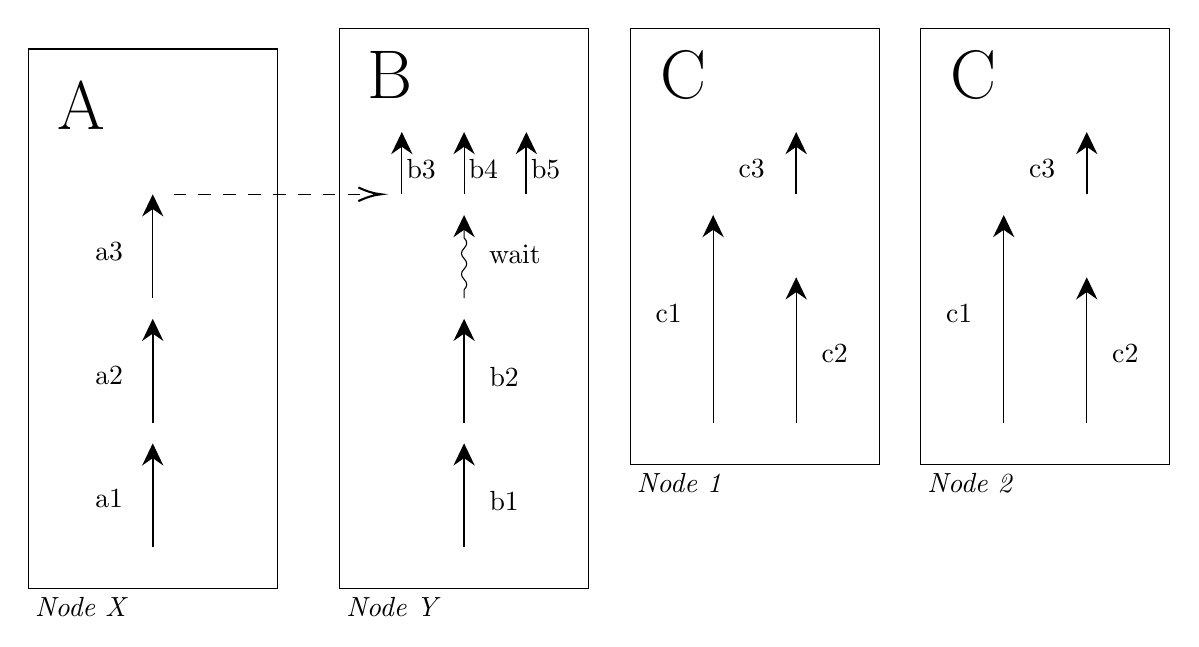
\begin{tikzpicture}[x=0.75pt,y=0.75pt,yscale=-1,xscale=1]
%uncomment if require: \path (0,320); %set diagram left start at 0, and has height of 320

%Straight Lines [id:da27430706126077264] 
\draw [color={rgb, 255:red, 0; green, 0; blue, 0 }  ,draw opacity=1 ][fill={rgb, 255:red, 255; green, 0; blue, 0 }  ,fill opacity=1 ][line width=0.75]    (80,263.5) -- (80,216.5) ;
\draw [shift={(80,213.5)}, rotate = 450] [fill={rgb, 255:red, 0; green, 0; blue, 0 }  ,fill opacity=1 ][line width=0.08]  [draw opacity=0] (10.72,-5.15) -- (0,0) -- (10.72,5.15) -- (7.12,0) -- cycle    ;
%Straight Lines [id:da18541775456344745] 
\draw [color={rgb, 255:red, 0; green, 0; blue, 0 }  ,draw opacity=1 ][fill={rgb, 255:red, 144; green, 19; blue, 254 }  ,fill opacity=1 ][line width=0.75]    (80,203.5) -- (80,156.5) ;
\draw [shift={(80,153.5)}, rotate = 450] [fill={rgb, 255:red, 0; green, 0; blue, 0 }  ,fill opacity=1 ][line width=0.08]  [draw opacity=0] (10.72,-5.15) -- (0,0) -- (10.72,5.15) -- (7.12,0) -- cycle    ;
%Straight Lines [id:da9191051295157292] 
\draw    (80,143.5) -- (80,96.5) ;
\draw [shift={(80,93.5)}, rotate = 450] [fill={rgb, 255:red, 0; green, 0; blue, 0 }  ][line width=0.08]  [draw opacity=0] (10.72,-5.15) -- (0,0) -- (10.72,5.15) -- (7.12,0) -- cycle    ;
%Straight Lines [id:da565354971469586] 
\draw [color={rgb, 255:red, 0; green, 0; blue, 0 }  ,draw opacity=1 ][line width=0.75]    (230,263.5) -- (230,216.5) ;
\draw [shift={(230,213.5)}, rotate = 450] [fill={rgb, 255:red, 0; green, 0; blue, 0 }  ,fill opacity=1 ][line width=0.08]  [draw opacity=0] (10.72,-5.15) -- (0,0) -- (10.72,5.15) -- (7.12,0) -- cycle    ;
%Straight Lines [id:da6700429327448342] 
\draw [color={rgb, 255:red, 0; green, 0; blue, 0 }  ,draw opacity=1 ][line width=0.75]    (230,203.5) -- (230,156.5) ;
\draw [shift={(230,153.5)}, rotate = 450] [fill={rgb, 255:red, 0; green, 0; blue, 0 }  ,fill opacity=1 ][line width=0.08]  [draw opacity=0] (10.72,-5.15) -- (0,0) -- (10.72,5.15) -- (7.12,0) -- cycle    ;
%Straight Lines [id:da28075371980457553] 
\draw [color={rgb, 255:red, 0; green, 0; blue, 0 }  ,draw opacity=1 ]   (200,93.5) -- (200,66.5) ;
\draw [shift={(200,63.5)}, rotate = 450] [fill={rgb, 255:red, 0; green, 0; blue, 0 }  ,fill opacity=1 ][line width=0.08]  [draw opacity=0] (10.72,-5.15) -- (0,0) -- (10.72,5.15) -- (7.12,0) -- cycle    ;
%Straight Lines [id:da9441221295165446] 
\draw [color={rgb, 255:red, 0; green, 0; blue, 0 }  ,draw opacity=1 ]   (230,93.5) -- (230,66.5) ;
\draw [shift={(230,63.5)}, rotate = 450] [fill={rgb, 255:red, 0; green, 0; blue, 0 }  ,fill opacity=1 ][line width=0.08]  [draw opacity=0] (10.72,-5.15) -- (0,0) -- (10.72,5.15) -- (7.12,0) -- cycle    ;
%Straight Lines [id:da3794379224544834] 
\draw [color={rgb, 255:red, 0; green, 0; blue, 0 }  ,draw opacity=1 ][line width=0.75]    (260,93.5) -- (260,66.5) ;
\draw [shift={(260,63.5)}, rotate = 450] [fill={rgb, 255:red, 0; green, 0; blue, 0 }  ,fill opacity=1 ][line width=0.08]  [draw opacity=0] (10.72,-5.15) -- (0,0) -- (10.72,5.15) -- (7.12,0) -- cycle    ;
%Straight Lines [id:da13857817807873274] 
\draw [color={rgb, 255:red, 0; green, 0; blue, 0 }  ,draw opacity=1 ]   (350,203.5) -- (350,106.5) ;
\draw [shift={(350,103.5)}, rotate = 450] [fill={rgb, 255:red, 0; green, 0; blue, 0 }  ,fill opacity=1 ][line width=0.08]  [draw opacity=0] (10.72,-5.15) -- (0,0) -- (10.72,5.15) -- (7.12,0) -- cycle    ;
%Straight Lines [id:da18881367347259226] 
\draw [color={rgb, 255:red, 0; green, 0; blue, 0 }  ,draw opacity=1 ]   (390,203.5) -- (390,136.5) ;
\draw [shift={(390,133.5)}, rotate = 450] [fill={rgb, 255:red, 0; green, 0; blue, 0 }  ,fill opacity=1 ][line width=0.08]  [draw opacity=0] (10.72,-5.15) -- (0,0) -- (10.72,5.15) -- (7.12,0) -- cycle    ;
%Straight Lines [id:da5578630098708864] 
\draw [color={rgb, 255:red, 0; green, 0; blue, 0 }  ,draw opacity=1 ][line width=0.75]    (390,93.5) -- (390,66.5) ;
\draw [shift={(390,63.5)}, rotate = 450] [fill={rgb, 255:red, 0; green, 0; blue, 0 }  ,fill opacity=1 ][line width=0.08]  [draw opacity=0] (10.72,-5.15) -- (0,0) -- (10.72,5.15) -- (7.12,0) -- cycle    ;
%Straight Lines [id:da19300882959893817] 
\draw  [dash pattern={on 4.5pt off 4.5pt}]  (90,93.5) -- (188,93.5) ;
\draw [shift={(190,93.5)}, rotate = 180] [color={rgb, 255:red, 0; green, 0; blue, 0 }  ][line width=0.75]    (10.93,-3.29) .. controls (6.95,-1.4) and (3.31,-0.3) .. (0,0) .. controls (3.31,0.3) and (6.95,1.4) .. (10.93,3.29)   ;
%Straight Lines [id:da8425704792181163] 
\draw [color={rgb, 255:red, 0; green, 0; blue, 0 }  ,draw opacity=1 ]   (490,203.5) -- (490,106.5) ;
\draw [shift={(490,103.5)}, rotate = 450] [fill={rgb, 255:red, 0; green, 0; blue, 0 }  ,fill opacity=1 ][line width=0.08]  [draw opacity=0] (10.72,-5.15) -- (0,0) -- (10.72,5.15) -- (7.12,0) -- cycle    ;
%Straight Lines [id:da4623771258590563] 
\draw [color={rgb, 255:red, 0; green, 0; blue, 0 }  ,draw opacity=1 ]   (530,203.5) -- (530,136.5) ;
\draw [shift={(530,133.5)}, rotate = 450] [fill={rgb, 255:red, 0; green, 0; blue, 0 }  ,fill opacity=1 ][line width=0.08]  [draw opacity=0] (10.72,-5.15) -- (0,0) -- (10.72,5.15) -- (7.12,0) -- cycle    ;
%Straight Lines [id:da01593649548581877] 
\draw [color={rgb, 255:red, 0; green, 0; blue, 0 }  ,draw opacity=1 ][line width=0.75]    (530,93.5) -- (530,66.5) ;
\draw [shift={(530,63.5)}, rotate = 450] [fill={rgb, 255:red, 0; green, 0; blue, 0 }  ,fill opacity=1 ][line width=0.08]  [draw opacity=0] (10.72,-5.15) -- (0,0) -- (10.72,5.15) -- (7.12,0) -- cycle    ;
%Straight Lines [id:da11733369284313999] 
\draw    (230,106.5) -- (230,114.5) .. controls (231.67,116.17) and (231.67,117.83) .. (230,119.5) .. controls (228.33,121.17) and (228.33,122.83) .. (230,124.5) .. controls (231.67,126.17) and (231.67,127.83) .. (230,129.5) .. controls (228.33,131.17) and (228.33,132.83) .. (230,134.5) .. controls (231.67,136.17) and (231.67,137.83) .. (230,139.5) -- (230,143.5) -- (230,143.5) ;
\draw [shift={(230,103.5)}, rotate = 90] [fill={rgb, 255:red, 0; green, 0; blue, 0 }  ][line width=0.08]  [draw opacity=0] (10.72,-5.15) -- (0,0) -- (10.72,5.15) -- (7.12,0) -- cycle    ;
%Shape: Rectangle [id:dp6987570624593641] 
\draw   (20,23.5) -- (140,23.5) -- (140,283.5) -- (20,283.5) -- cycle ;
%Shape: Rectangle [id:dp026922254453187522] 
\draw   (170,13.5) -- (290,13.5) -- (290,283.5) -- (170,283.5) -- cycle ;
%Shape: Rectangle [id:dp3707896533993156] 
\draw   (310,13.5) -- (430,13.5) -- (430,223.5) -- (310,223.5) -- cycle ;
%Shape: Rectangle [id:dp19211708743148737] 
\draw   (450,13.5) -- (570,13.5) -- (570,223.5) -- (450,223.5) -- cycle ;

% Text Node
\draw (45.5,51) node  [font=\Huge] [align=left] {A};
% Text Node
\draw (194.5,36) node  [font=\Huge] [align=left] {B};
% Text Node
\draw (335.5,36) node  [font=\Huge] [align=left] {C};
% Text Node
\draw (475.5,36) node  [font=\Huge] [align=left] {C};
% Text Node
\draw (254.5,122.5) node   [align=left] {wait};
% Text Node
\draw (51,234.5) node [anchor=north west][inner sep=0.75pt]   [align=left] {a1};
% Text Node
\draw (51,175.5) node [anchor=north west][inner sep=0.75pt]   [align=left] {a2};
% Text Node
\draw (51,115.5) node [anchor=north west][inner sep=0.75pt]   [align=left] {a3};
% Text Node
\draw (241,235.5) node [anchor=north west][inner sep=0.75pt]   [align=left] {b1};
% Text Node
\draw (241,175.5) node [anchor=north west][inner sep=0.75pt]   [align=left] {b2};
% Text Node
\draw (201,75.5) node [anchor=north west][inner sep=0.75pt]   [align=left] {b3};
% Text Node
\draw (231,75.5) node [anchor=north west][inner sep=0.75pt]   [align=left] {b4};
% Text Node
\draw (261,75.5) node [anchor=north west][inner sep=0.75pt]   [align=left] {b5};
% Text Node
\draw (321,145.5) node [anchor=north west][inner sep=0.75pt]   [align=left] {c1};
% Text Node
\draw (401,164.5) node [anchor=north west][inner sep=0.75pt]   [align=left] {c2};
% Text Node
\draw (361,75.5) node [anchor=north west][inner sep=0.75pt]   [align=left] {c3};
% Text Node
\draw (461,145.5) node [anchor=north west][inner sep=0.75pt]   [align=left] {c1};
% Text Node
\draw (541,164.5) node [anchor=north west][inner sep=0.75pt]   [align=left] {c2};
% Text Node
\draw (501,75.5) node [anchor=north west][inner sep=0.75pt]   [align=left] {c3};
% Text Node
\draw (22,286.5) node [anchor=north west][inner sep=0.75pt]   [align=left] {\textit{Node X}};
% Text Node
\draw (172,286.5) node [anchor=north west][inner sep=0.75pt]   [align=left] {\textit{Node Y}};
% Text Node
\draw (312,226.5) node [anchor=north west][inner sep=0.75pt]   [align=left] {\textit{Node 1}};
% Text Node
\draw (452,226.5) node [anchor=north west][inner sep=0.75pt]   [align=left] {\textit{Node 2}};


\end{tikzpicture}
}
        \end{minipage}
      } \label{fig:intra-comp-tasks}
    }
    \caption{Examples to illustrate the four parallelism levels
      considered in this paper}
    \label{fig:parlevels}
  \end{center}
\end{figure*}

%\SR{Give a reason to exclude declarative approaches, \eg worse/hard to measure performance}

Metrics for SE and parallelism are suitable for procedural approaches,
as they consider \emph{tasks} and not \emph{resources}. This excludes
\puppet or \salt, for instance. While declarative approaches have great
advantages, they are not considered in this paper. Indeed we put a strong emphasis on parallelism in this paper. This requires a fine-grain definition of deployments, at the level of tasks. Declarative approaches on the contrary raise the abstraction level at the price of flexibility.

\paragraph{Formalism}
The metric considered here is the existence of a formal model for each
commissioning solution. Indeed, we claim that formal study of
commissioning models and of their semantics is required for
verification and safety in deployments. For instance, the formal model
of \mad has been successfully used to verify safety properties on
distributed software commissioning by model checking, as presented
in~\cite{coullon:hal-02323641}.

%----------------------------
\subsection{Description and comparison of the related work}
% ----------------------------

We have selected 8 distributed software commissioning solutions for a
deeper comparison, including production tools (in particular those
with a significant open source community) and academic solutions.
%
%% The selection is made of 8 works selected from the five classes
%% introduced in Section~\ref{sec:rwclasses}: \shell, \fractal, \ansible,
%% \deployware, \aeolus, \juju, \tosca and \kubernetes.

% Shell-scripts
\paragraph{Shell scripts}
Traditionally, operators automate software commissioning by
transcribing actions and configurations from README files and
tutorials into a sequence of commands in shell scripts. On the one
hand, those scripts are written with low-level imperative languages,
and with good programming skills, it is possible to express complex
workflows (\eg idempotency, parallelism, remote actions using
SSH). For instance, parallelism can be managed by combining command
execution in the background (\eg using the control operator \& in
\bash) and synchronization commands such as \texttt{wait}. On the
other hand, as the system grows, any custom script becomes
error-prone, unpredictable, hard to understand and to maintain. Shell
scripts lack software engineering aspects and offer no framework to
express modules or tasks and their dependencies, thus hindering
separation of concerns. Table~\ref{tab:comparison} indicates that the
features corresponding to our metrics can be implemented manually with
shell scripts. Of course, this implementation is difficult, error-prone, and
time-consuming.
% devstack is a set of shell script to deploy OpenStack on a single machine

\paragraph{Fractal}
In the Object Management Group's (OMG)
specification~\cite{ccmdeploy:omg06}, the commissioning model is rigid
and fixed by the model. In \fractal~\cite{Blair2009} and its
evolutions GCM and GCM/ProActive~\cite{baude:hal-01001043}, the
control of a component (\eg its commissioning) is decoupled from its
functionalities into a so called \emph{membrane} which is itself
described as a component assembly written in Java. The membrane is
handled by the \fractal runtime but the sub-assembly and its
associated codes are entirely left to the user. That is why in
Table~\ref{tab:comparison}, feature not natively supported by \fractal
are shown manually implementable, using Java. Both \emph{separation of
  concerns} and \emph{inter-comp} are well handled by \fractal thanks
to the notion of port (dependencies within the component or with other
components) adapted to the membrane. Note that only \fractal
components are supported, but the commissioning of existing
modules can be encapsulated in a \fractal component.

% Deployware
\paragraph{Deployware}
\citeauthor{flissi2008ccgrid} proposed \deployware (DW), a research
effort targetting distributed software commissioning in the context of
Grid computing~\cite{flissi2008ccgrid}. Its implementation is based on
the \fractal model. A component is called a \emph{personality} and is
associated with a fixed set of commissioning actions: install,
configure, start, manage, stop, unconfigure and uninstall. Each action
describes a sequence of tasks, written in a specific high-level
language that uses pre-defined instructions (\eg execute command, copy
a file). While there is no notion of component ports, it is possible
to express dependencies between components to initiate automatic
coordination. For instance, when the operator triggers the action
"install" on a component, the same action is triggered recursively to
its dependencies. Because some features are not entirely controlled by
the user, metrics \emph{tasks}, \emph{SIMH} and \emph{inter-comp} are
considered partially supported by \deployware. Finally, \deployware is
based on \fractal and a formal effort has been carried out on
\fractal, therefore the formal aspect support of \deployware is
considered partial.

% Ansible
\paragraph{Ansible}
For devops used to shell scripts, \ansible has become a popular
configuration management tool, since it relies on a simple syntax
written in YAML and does not require agents on administrated
servers. Tasks are managed using only SSH and Python, which are
commonly installed on every Linux distribution. In comparison, similar
tools such as \chef, \puppet or \cfengine not only require some
understanding of Ruby or a custom language, but they are built on an
agent-based architecture and require prior agent commissioning on
remote hosts. \ansible improves separation of concerns by defining
\emph{roles}, which can be seen as software components. Each role
contains files that describe a sequence of tasks. To define a
composition, a specific file called an \ansible \emph{playbook} is
used to map the desired roles to the groups of nodes they will be
applied to. Those groups of nodes are defined in a separate file
called the \emph{inventory}. When \ansible is triggered, roles and
their related tasks are sequentially executed to the associated groups
of nodes. While tasks declarations are indeed managed sequentially,
each task is executed in parallel when mapped to multiple remote
hosts, thus offering \emph{SIMH} support. Typically, an operator who
wants to commission an \apache web server and a \mysql database would
download two roles from Ansible Galaxy and register them in a
playbook. Since \ansible triggers roles in a sequential manner, if the
operator is not aware that the database must be commissioned before
the web server, she could make a mistake in the order of the roles she
declared. This makes the \emph{separation of concerns} support only
partial. Finally, as one of the possible types of tasks in \ansible is
the execution of a shell command, any script could be executed as a
task, thus allowing manually support for \emph{intra-comp-tasks}
parallelism.

% Tasks are declared in an imperative way, however, Ansible relies heavily on
% declarative modules, most of which ensure task idempotency (operations are run
% once even if called multiple times).

% Aeolus
\paragraph{Aeolus}
\citeauthor{dicosmo2014ic} proposed \aeolus, a formal component-based
model for the cloud~\cite{dicosmo2014ic}. Their component model
captures the internal states of a component commissioning process
thanks to a finite state machine. Each state can be connected to use,
provide, or conflict ports to declare dependencies between the
commissioning steps of different components. Hence, ports enable
correct coordination of the global deployment process. The deployment
procedure should then be written by the user or by an external
tool~\cite{dicosmo:hal-01233489} as a sequence of actions
leading to a different state. As a result, the internal of each
component must be known. For this reason, \emph{separation of
  concerns} support is only partial. Furthermore as the deployment
procedure is a sequence and as parallel transitions cannot be defined
the \emph{intra-comp-tasks} parallelism level is only possible in a
manual way (not automated).

% Juju
\paragraph{Juju}
Canonical has developed their own software commissioning solution,
\juju\footnote{\url{https://jujucharms.com/}}, which aims at commissioning any
kind of application on various cloud providers (\eg AWS,
OpenStack) and types of resources (container, VM or
bare-metal). Its concepts are close to those of component
models. Software modules are packaged as \juju \emph{charms} that
describe the software commissioning steps through a set of scripts
called
\emph{hooks}. Operators define their composition in a specific file
called \emph{bundle} in which they declare the desired charms with
their \emph{relations}. A relation is declared between two charms and
used for component synchronization (by triggering hooks) and data
sharing at runtime, similarly to component ports. As the concepts
behind \juju resemble those of \aeolus, the metrics are similar with
the exception of the formal aspect.
% good soc, download charms and run juju deploy

\begin{table*}[tp]
  \centering
  \small
  

% \begin{tabular}{cl|cccccc}
%     \toprule
%     & & Shell & Ansible & DW & K8S & Juju & Aeolus \\
%     \midrule
%     %\rowcolor{gray!15}
%     \multirow{3}{*}{\STAB{\rotatebox[origin=c]{90}{Parallel}}}
%     & node    & \checkmark & \checkmark & \checkmark & \checkmark & \checkmark & \checkmark \\
%     & inter   & \checkmark &   &   &   & \checkmark & \checkmark \\
%     %\rowcolor{gray!15}
%     & intra   & \checkmark &   &   &   &   &   \\
%     \midrule
%     \multirow{2}{*}{\STAB{\rotatebox[origin=c]{90}{SE}}}
%     & module  &   & \checkmark & \checkmark & \checkmark & \checkmark & \checkmark \\
%     %\rowcolor{gray!15}
%     & ports   &   &   &   &   & \checkmark & \checkmark \\
%     \bottomrule
% \end{tabular}

% \newcolumntype{g}{>{\columncolor{gray!15}}c}
% \begin{tabular}{cl|gc|gcgc|gc|g}
%   \toprule
%   \rowcolor{white}
%   & & \multicolumn{2}{c|}{\textit{Coding}} & \multicolumn{4}{c|}{\textit{Software configuration}} & \multicolumn{2}{c|}{\textit{Provisioning}} & \textit{Orchestration} \\
%   \midrule
%   & & \shell & \fractal & \textbf{\ansible} & \puppet & \deployware & \textbf{\aeolus} & \juju & \tosca & \kubernetes \\
%   & & & \cite{} & \cite{} & \cite{} & \cite{} & \cite{} & \cite{} & \cite{} & \cite{} \\ 
%   \midrule
%   \multirow{4}{*}{\STAB{\rotatebox[origin=c]{90}{Soft. eng.}}}
%   & components & M & \checkmark & \checkmark & \checkmark & \checkmark & \checkmark & \checkmark & \checkmark & \checkmark \\
%   & tasks & M & M & \checkmark & M & (\checkmark) & \checkmark & \checkmark & M & \\
%   & resources & M & M & & \checkmark & & & & \checkmark & \\
%   & sep. of con. & M & (\checkmark) & (\checkmark) & \checkmark & \checkmark & (\checkmark) & (\checkmark) & \checkmark & \checkmark \\
%   \midrule
%   \multirow{5}{*}{\STAB{\rotatebox[origin=c]{90}{Parallelism}}}
%   & SIMH & M & (\checkmark) & \checkmark & \checkmark & (\checkmark) & \checkmark & \checkmark & (\checkmark)& \checkmark\\
%   & inter-comp & M & (\checkmark) & & & (\checkmark) & \checkmark & \checkmark & (\checkmark)& (\checkmark)\\
%   & inter-task & M & M & & & & \checkmark & \checkmark & & \\
%   & inter-resource & M & M & & (\checkmark) & & & & (\checkmark) & \\
%   & intra-task & M & M & M & M & M & M & M & M & \\
%   \midrule
%   & formal & & \checkmark & & & (\checkmark) & \checkmark & & \checkmark & \\
%   \midrule
%   & score & 9 & 17 & 11 & 14 & 14 & 20 & 17 & 18 & 11\\
%     \bottomrule
% \end{tabular}

% without resources and puppet

\newcolumntype{g}{>{\columncolor{gray!15}}c}
\begin{tabular}{cl|gc|gcg|cg|c}
  \toprule
  \rowcolor{white}
  & & \multicolumn{2}{c|}{\textit{Coding}} & \multicolumn{3}{c|}{\textit{Software configuration}} & \multicolumn{2}{c|}{\textit{Infrastructure}} & \textit{Orchestration} \\
  \midrule
  & & \shell & \fractal & \deployware & \ansible & \aeolus & \juju & \tosca & \kubernetes \\
  & & & \cite{Baude,Blair2009,baude:hal-01001043} & \cite{flissi2008ccgrid} & \cite{ansible:web} & \cite{dicosmo:hal-01233489,dicosmo2014ic,zwolakowski:tel-01172022} & \cite{juju:web} & \cite{tosca:web,brogi2018,7561358,8599581} & \cite{kubernetes:web,43826} \\ 
  \midrule
  \multirow{3}{*}{\STAB{\rotatebox[origin=c]{90}{SE}}}
  & components & M & \checkmark & \checkmark & \checkmark & \checkmark & \checkmark & \checkmark & \checkmark \\
  & tasks & M & M & (\checkmark) & \checkmark & \checkmark & (\checkmark) & M & - \\
  & sep. of con. & M & \checkmark & \checkmark & (\checkmark) & (\checkmark) & (\checkmark) & \checkmark & \checkmark \\
  \midrule
  \multirow{4}{*}{\STAB{\rotatebox[origin=c]{90}{Parallel}}}
  & SIMH & M & \checkmark & (\checkmark) & \checkmark & \checkmark & \checkmark & (\checkmark)& \checkmark\\
  & inter-comp & M & \checkmark & (\checkmark) & - & \checkmark & \checkmark & (\checkmark)& (\checkmark)\\
  & inter-comp-tasks & M & M & - & - & \checkmark & (\checkmark) & - & - \\
  & intra-comp-tasks & M & M & M & M & M & M & M & - \\
  \midrule
  & formal & - & \checkmark & (\checkmark) & - & \checkmark & - & \checkmark & -\\
  \midrule
  & score & 7 & 18 & 15 & 12 & 21 & 16 & 15 & 11\\
    \bottomrule
\end{tabular}



  \caption{Comparison of commissioning solutions based on aspects
  regarding software engineering (SE), parallelism and formalism. A supported metric is denoted
  \checkmark and counts for 3 points in the score; a partially
  supported metric is denoted (\checkmark) and counts for 2 points; a manually supported metric is denoted \emph{M} and counts for 1 point; and finally a non-supported metric is denoted -.}
  \label{tab:comparison}
\end{table*}

\paragraph{TOSCA}
The \emph{Topology and Orchestration Specification for Cloud
Applications} (TOSCA) is another component-oriented model that
partially addresses the commissioning of its
components. TOSCA~\cite{tosca:web,brogi2018} is a standardization
effort from OASIS to describe cloud applications, their components and
their deployment artifacts, using standard languages (\ie XML,
YAML). A TOSCA description (or template) corresponds to a graph where
nodes represent TOSCA resources (\eg software components, virtual
machines, physical servers), and where edges represent the relations
between these nodes. Artifacts (of any type: scripts, executable etc.)
can be added to TOSCA descriptions in a CSAR (Cloud Service ARchive)
to detail commissioning steps. Those commissioning steps can thus be
customized by the developer, but there is no model, nor any guarantees
associated with them. Therefore, the feature associated with
the \emph{tasks} and \emph{intra-comp-tasks} metrics can be handled
manually by the user. As there is no way to declare dependencies
between artifacts of components, \emph{inter-task} parallelism is not
supported, however, relations between components make both \emph{SIMH}
and \emph{inter-comp} parallelism theoretically available
in \tosca. No information has been found on the complete support of
these features in \tosca
implementations~\cite{cloudify:web,opentosca:web}. Finally, the \tosca
standard~\cite{7561358} is formally defined to an extent.

% Kubernetes
\paragraph{Kubernetes}
Initiated by Google, \kubernetes (K8S) is a popular framework to
commission distributed software in the form of microservices that are
packaged as a hierarchy of Docker containers and \emph{pods}. A
software component in \kubernetes is defined as a Docker
container. These components have no ports to manage coordination, and
their internals are fixed, since containers can only be started and
stopped. As a consequence, the commissioning process is
error-prone. For instance, a web server can be started before the
required database and thus fail. For this reason, \emph{inter-comp}
parellelism is only partially supported. \kubernetes requires
container to be started in any order, therefore any container must
embed a waiting procedure w.r.t.\ its dependencies. If the deployment of
a container fails, \kubernetes automatically retries. For stateless
microservice architectures, this deployment strategy is popular.

%----------------------------
\subsection{Discussions}
%----------------------------
% 3. discussion
% - flexibility vs automation vs formal
% - separation of concerns
% - intra-task parallelism
% - performance model and formal

We have compared eight solutions according to software engineering metrics, parallelism metrics and one metric regarding the formal definition of the considered solution. Table~\ref{tab:comparison} summarizes this comparison and raises a few key points that we discuss in the following section.

As usual when working on programming languages, the existing tools
illustrate the difficult trade-off between flexibility and
automation. On the one hand, when the tool is highly programmable,
developers have the ability to manage their own code organization and
to handle any kind of software engineering or efficiency property. For
instance, by using shell scripts, any feature that we took into
account could be handled. However, each of them would have to be
hand-coded, which is difficult and error-prone. On the other hand,
some solutions such as \deployware and \juju restrict the internal
commissioning behavior of components to a fixed set of actions (\eg
install, configure, start). This guarantees full control of the
automated parallelism level, but also prevents potential optimizations
allowed by the specifics of each component.

\aeolus is the solution with the highest score according to our
metrics. Indeed, \aeolus combines advantages of component models to
structure the code of software commissioning and enhance its
separation of concerns, while introducing an additional way to model
the internal commissioning behavior of each component through
tasks. It seems that \aeolus offers a good trade-off between
flexibility and automation. However, it handles only partial
separation of concerns.

Furthermore, no existing solution offers full support for
\emph{intra-comp-tasks} parallelism. Although a few solutions already
offer a way to model the internal commissioning behavior of each
component by using tasks, dependencies between those tasks are limited
to a sequential order, thus making \emph{intra-comp-tasks} parallelism
impossible. This could be handled manually in some of the existing
tools, however these parallel aspects are difficult to implement, and
should preferably be handled automatically.

Although introducing more parallelism opens up potential performance
gains, it also introduces more complexity for the user. For this
reason, formalizing the commissioning solution is of high importance
to guarantee properties of the commissioning, such as attainability.

% One further aspect of the level of programmability provided by commissioning
% tools. When the tool is highly programmable, developers have the ability to
% manage their own code organization. This is an important aspect to finely
% express what can be executed in parallel (thus it impacts performance). For
% instance \deployware and \juju limit the internals of their modules to a
% predefined set of actions (eg config, install) while such actions might contain
% instructions that can be declared parallelable.
% %
% Our solution differs by letting developers abstract a set of instructions in the
% form of transitions. Transitions can be expressed in parallel, and their
% synchronisation is declared using states.
% %high programmable can also  improve maintainability by isolating specfic code
% %in a transition.

% Finally, a desired feature for distributed software commissioning is automation.
% Typically an operator should download the desired modules to compose a
% distributed software, instantiate and connect them through their ports, then run
% the commissioning process. This aspect requires an operational semantic to
% express how the commissioning process automatically progresses with respect to
% inter and intra-component dependencies. For instance, \aeolus, which supports
% only inter-component parallelism, is a component-based model that relies on
% states and transitions to manage inter-component dependencies. However, since
% the model lacks an operational semantic, each operation is planned and executed
% by an external scheduler. In this work, one of our contribution is to provide a
% operational semantic which drives the execution of the distributed software
% commissioning, and will be explained in \cref{subsec:operational_semantics}.

% As depicted in~\cref{tab:comparison}, we can conclude from this analysis that
% individually, none of the above attempts adequately provide a commissioning tool
% which can express both a high-degree of parallelism and feature software
% engineering aspects like separation of concerns.
% In the rest of this paper, we define \mad, our contribution which is inspired by
% \aeolus as a component-based model and relies on modules and ports to express all
% the parallelism levels described above. In the rest of the paper, we will
% focus the comparison of our solution with \ansible and \aeolus, since the former
% is widely used in production, while the second is a research effort that
% provides most of the above features.



%-------------------------------------------------------
\section{Overview}
\label{sec:mad_model}
%-------------------------------------------------------
% \begin{itemize}
% \item component-based commissioning model
% \item control components to handle the commissioning of any existing
%   component in any language
% \item goals: programmable, composable, reusable, efficient
% \item composed of:
%   \begin{itemize}
%   \item meta-model
%   \item graphical language
%   \item concrete language
%   \item formal specification (next section)
%   \item formal operational semantics (next section)
%   \end{itemize}
% \item meta-models of assembly and components (add groups)
% \item example Apache/MariaDB with graphical and concrete syntax
% \item simplified explanation of the operational semantics (middleware)
% \item discussion on the goals
% \end{itemize}

%%%%%%%%%%%%%%%%%%%%%%%%%%
\subsection{Principles}

\mad is a procedural \emph{configuration tool} relying on a
component-based coordination model for commissioning
procedures. Inspired by \aeolus, it enhances automation, separation of
concerns and level of parallelism for distributed software
commissioning. Usually, component models are used to write distributed
software in a modular fashion with guarantees on composition,
thus improving separation of concerns between developers, promoting
reuse of existing pieces of code, and enhancing flexibility and
maintainability of code. \mad brings these properties to commissioning
design instead of functional code design.

A \mad component is called a \emph{control} component, as it is only
intended to model the commissioning procedure of an already existing
piece of software code (functional component, module or service). A
\mad control component is a type containing an internal net inspired by Petri
nets, where places represent milestones of the commissioning, and
transitions between places represent actions to be performed (\eg
\texttt{apt-get install}, \texttt{docker pull}, etc.). If multiple
transitions leave a place, their parallel execution is automatically
handled and synchronized by \mad. A component may have dependencies
with other components. These dependencies are declared through ports,
a well-known concept in component-based software engineering. Two
types of ports, working in pairs, are available in \mad:
\emph{provide} and \emph{use} ports. However, both are
\emph{coordination} ports, \ie they model dependencies or
synchronization but do not implement them. By using coordination
ports, each component type can be defined independently and component
instances can be connected later by another developer, thus improving
separation of concerns and reusability of commissioning procedures. A
provide coordination port is bound to sets of places that represents
the milestones that have to be reached for the service or data to be
offered. Finally, use coordination ports are bound to one or multiple
transitions where data and service is actually required.

The overall commissioning procedure of a distributed software system
is built by composition in an \emph{assembly}, where component types
are instantiated and connected. All control components execute
simultaneously, thus introducing inter-component parallelism, in
addition to the intra-component parallelism offered by parallel
transitions. Two components connected by their respective compatible
ports will automatically be coordinated so that a component cannot use
a service or data if the associated provide port is not enabled.

\mad offers the expressiveness required to design composable and parallel
commissioning procedures for complex distributed software systems.

\begin{figure}[tbp]
  \begin{center}
    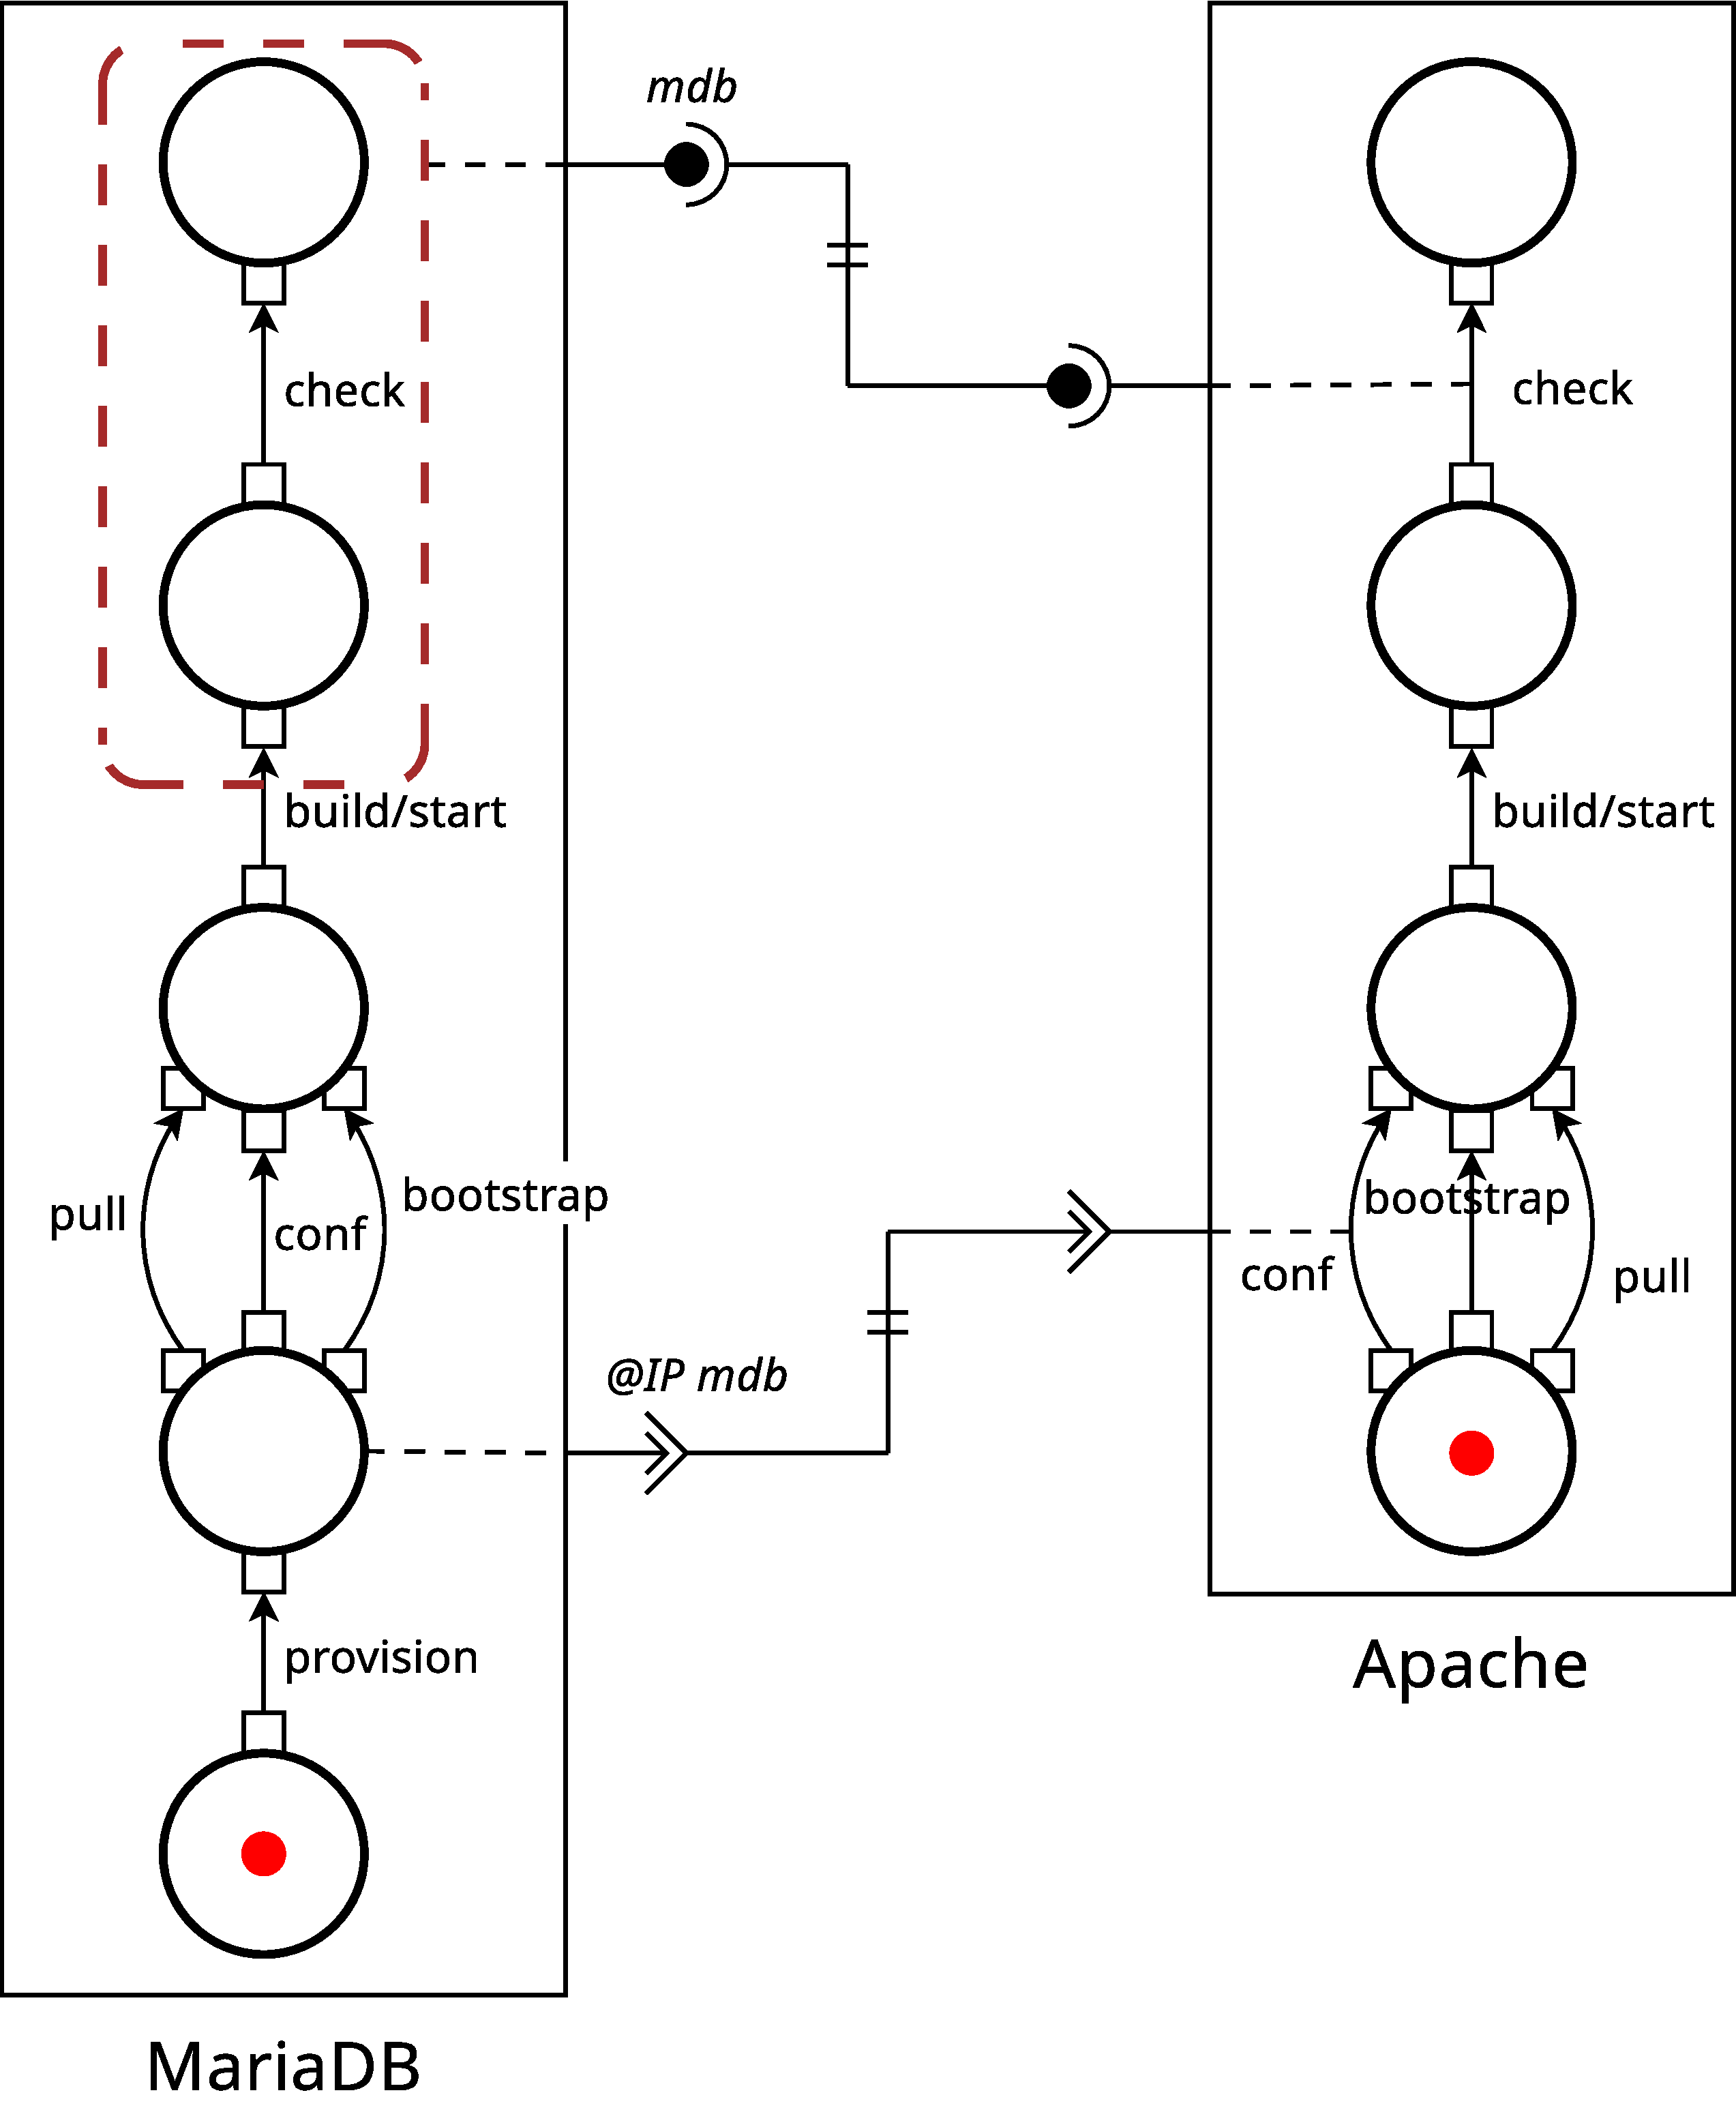
\includegraphics[width=0.7\linewidth]{./images/apachebdd.pdf}
  \end{center}
  \caption{Example of a \mad commissioning assembly with two components
    Apache and MariaDB. Places are represented by circles, with attached
    docks represented by small squares. Transitions are represented
    by arrows between the docks, and service ports by small black circles and
    semi-circles, data ports by outgoing or incoming arrows from
    components. \revised{Bindings of coordination ports are represented by dashed lines between a port and the places and transitions it is bound to. Tokens (in red) are placed in the initial
    places of each components in this example.}}
  \label{fig:example}
\end{figure}

\paragraph{Example}{
	Figure~\ref{fig:example} depicts a \mad commissioning assembly of an Apache 
	web server and a MariaDB database, using the graphical notation of \mad. 
	This example is based on a real container-based deployment described by 
	RedHat\footnote{\url{https://access.redhat.com/documentation/en-us/red_hat_enterprise_linux_atomic_host/7/html/getting_started_with_containers/install_and_deploy_an_apache_web_server_container}}\footnote{\url{https://access.redhat.com/documentation/en-us/red_hat_enterprise_linux_atomic_host/7/html/getting_started_with_containers/install_and_deploy_a_mariadb_container}}.
	 Two \mad control components are declared in this example: Apache and MariaDB. 
	Apache contains four places (white circles), or milestones, while MariaDB 
	contains five places. Some parallel transitions are declared for each of the 
	component and can be observed in the figure (parallel arrows). Both components 
	have two coordination ports. MariaDB provides both data and a service, while 
	Apache uses a service and data. These instances are connected by their ports. 
	Indeed, the Apache configuration depends on the IP address of the MariaDB 
	component, and the testing phase for Apache, called \texttt{check}, uses the 
	MariaDB service. \revised{Each coordination port is bound to internal elements. This is depicted by a dashed line between ports and places or transitions. For instance, the provide port \texttt{@IP mdb} is bound to the second place of the MariaDB component, and the first use port of the component Apache is bound to the transition \texttt{conf}}.
} %\CP{Ne faut il pas dire quelque part que les ports ne passent que les info de synchro et pas les données/services eux-même ? Par exemple est-ce \mad qui transfére les données comme l'@IP mdb?}

\mad involves two kinds of actors. First is the \emph{developer} of a
control component, who may be the author of the associated existing
piece of code, another developer, or even a system operator or
administrator. Second is the \emph{devops} engineer who designs an
assembly, \ie writes the overall commissioning procedure of a
distributed software system to deploy on an infrastructure. \mad
offers clear separation of concerns between the commissioning of a
single component on the one hand, and the composition of an assembly
on the other. The latter does not require detailed information about
the commissioning of each component. This is a benefit compared to
existing solution. For instance, even if Ansible offers properties
close to composition (\eg roles, playbooks, tasks, etc.), the devops
still has to determine the correct order of composition. By contrast,
the correct coordination, hence the correct order of execution, is
automatically guaranteed by the \mad semantics and the composition of
the component instances. Composition is illustrated in
Figure~\ref{fig:simple} where the details of each component, since
they are not needed, are omitted. This type of property is also
offered by Aeolus~\cite{dicosmo2014ic}, albeit without parallelism
within components.

\begin{figure}[tbp]
  \begin{center}
    
\includegraphics[width=0.6\linewidth]{./images/simpleass2.pdf}
  \end{center}
  \caption{\mad assembly of an Apache component and a MariaDB
    component without knowing the details of each component.}
  \label{fig:simple}
\end{figure}

The formalization of \mad will be detailed in
Section~\ref{sec:formal_model}.

%%%%%%%%%%%%%%%%%%%%%%%%%%
% \subsection{Meta-model}

% \HC[Maverick]{figures a refaire avec nos discussions}

% \begin{figure}[tbp]
%   \begin{center}
%     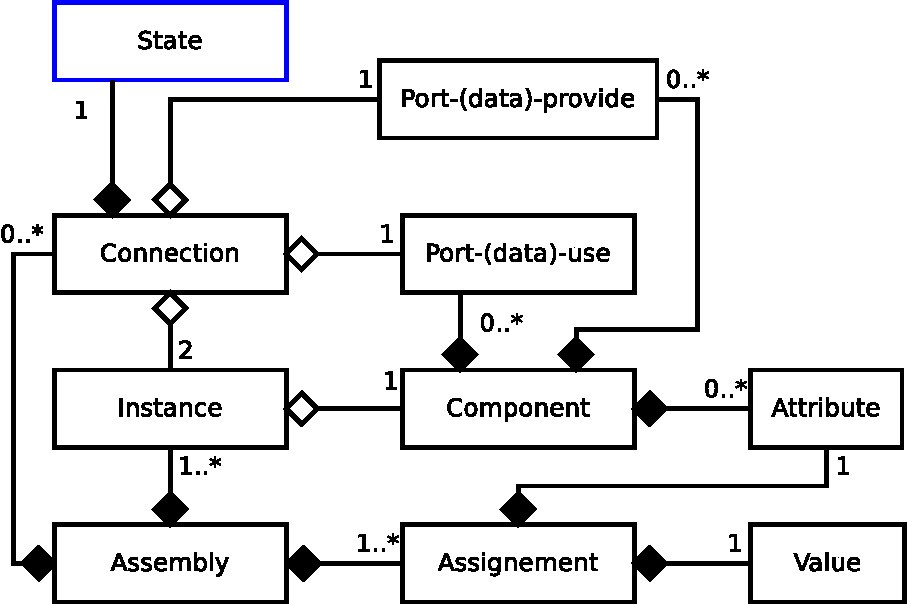
\includegraphics[width=0.9\linewidth]{./images/ass_uml.pdf}
%   \end{center}
%   \caption{\mad meta-model of an assembly, \ie an overall
%     commissioning procedure of a distributed software.}
%   \label{fig:mmass}
% \end{figure}

% Figures~\ref{fig:mmass} and~\ref{fig:mmcomp} respectively depict the
% UML diagram representing the \mad meta-model of an assembly, and the
% meta-model of a component. A \mad assembly is not different from a
% usual assembly in any component model of the literature. An assembly
% basically contains component instances, connected to each other
% through their compatible ports. One specificity is that \mad handles
% four types of ports instead of usually two, by dissociating service
% ports from data ports, each having their own semantics. Intuitively,
% unlike service ports, data ports act as data registries thus, once
% activated, they will remain active forever.

% \begin{figure}[tbp]
%   \begin{center}
%     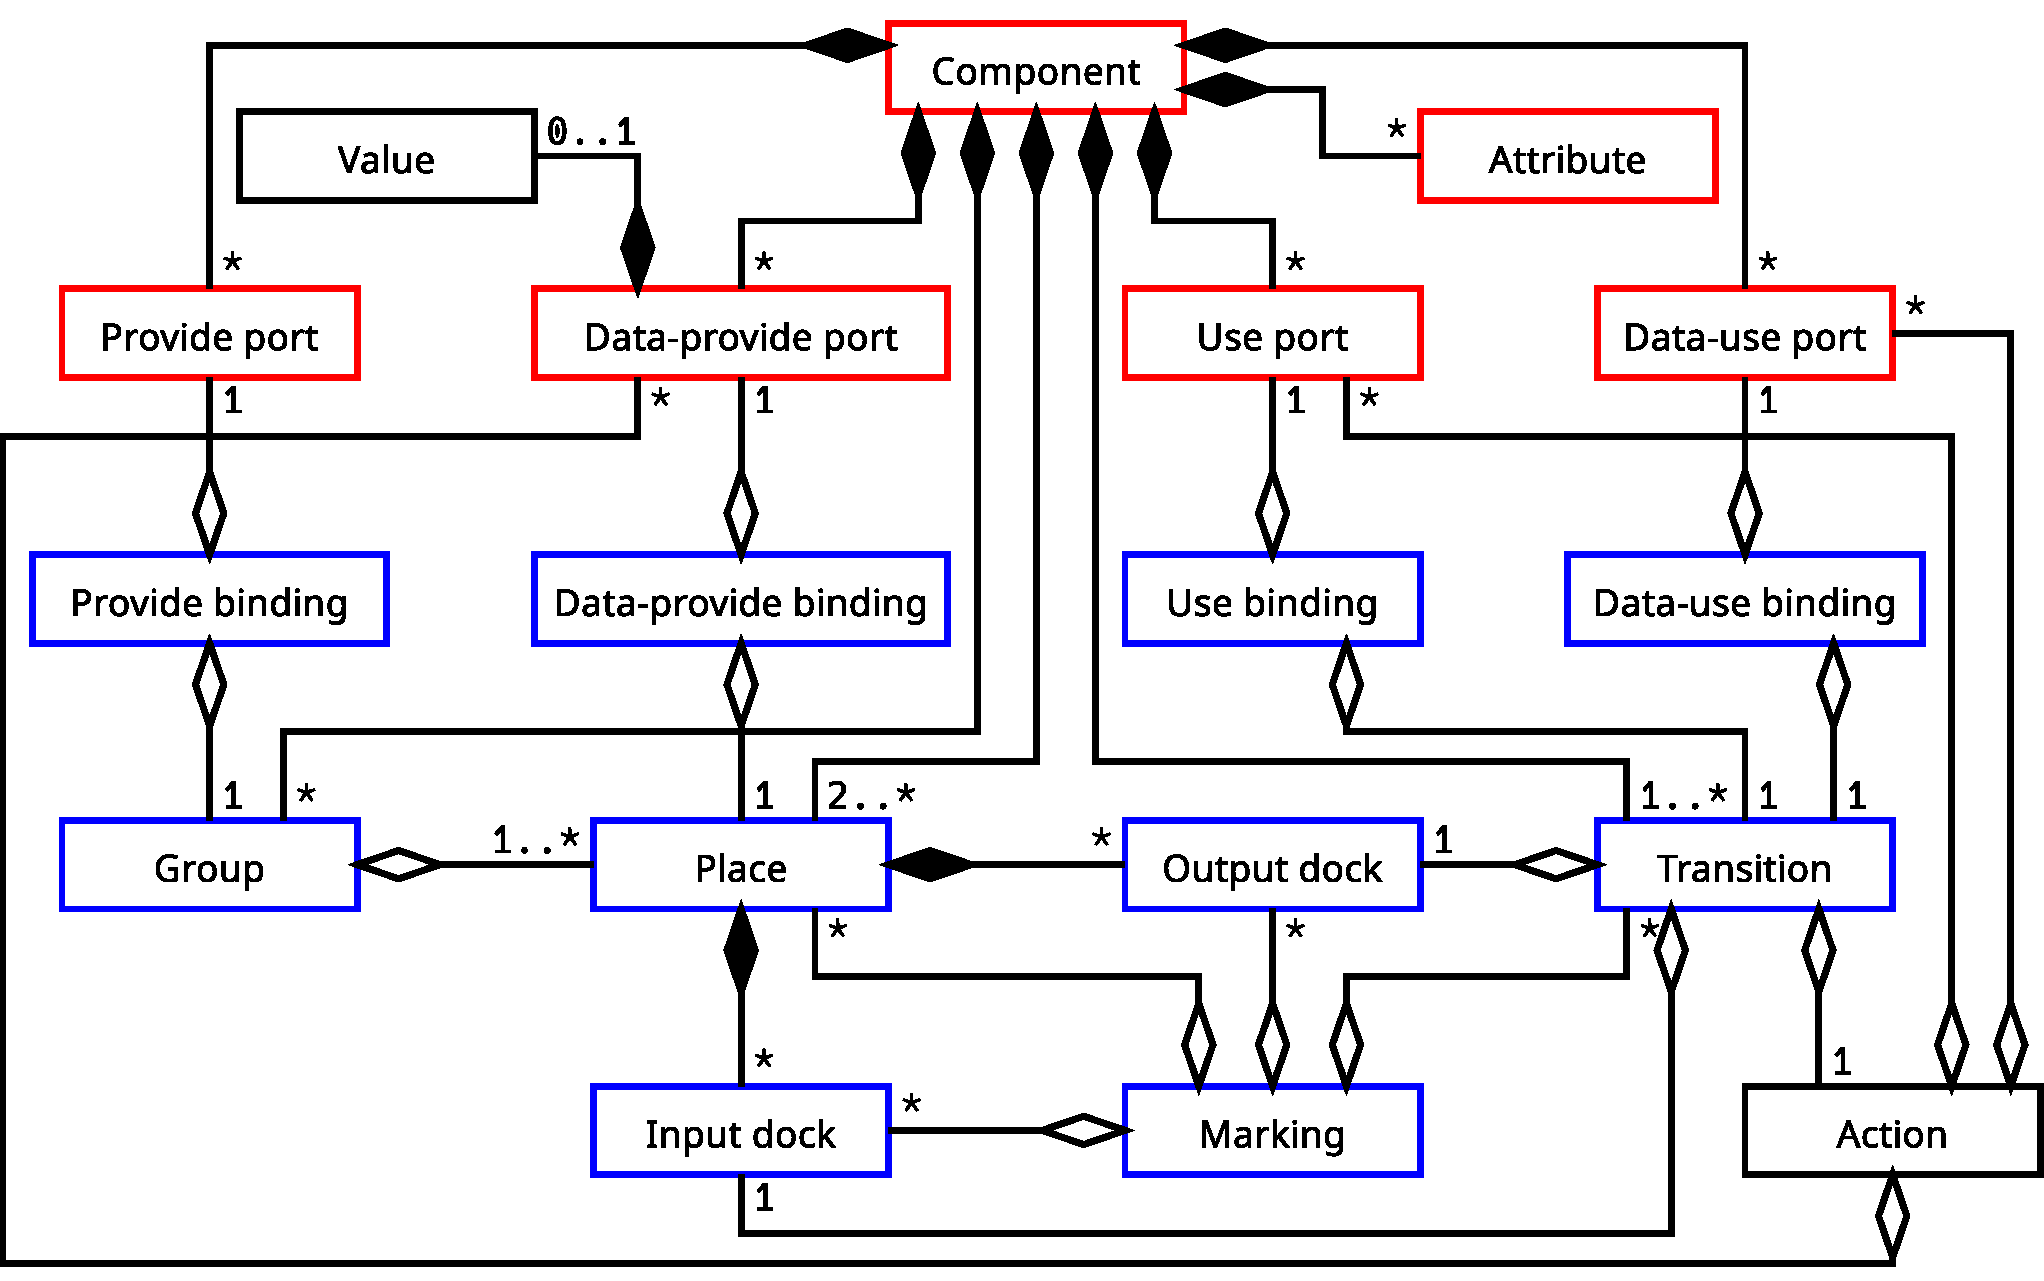
\includegraphics[width=0.9\linewidth]{./images/component_uml.pdf}
%   \end{center}
%   \caption{\mad meta-model of a component, \ie the commissioning
%     procedure of a single component (\ie module or service).}
%   \label{fig:mmcomp}
% \end{figure}

% However, as already explained a \mad component is very different
% from usual components in the literature. A component type contains a
% set of places, a set of transitions, and a set of service-provide,
% service-use, data-provide and data-user ports.
% Service-provide ports (service or data) are bound to groups of
% places. Those groups of places represent the sub-part of the
% commissioning procedures where a given service is provided. A
% data-provide port is simply bound to one place from which the data is
% provided. Use ports (data or service) are bound to transitions where
% the corresponding data or services modeled by ports are actually used
% by the code executed by the transition.

%%%%%%%%%%%%%%%%%%%%%%%%%%
\subsection{Concrete language}

\mad also comes with a prototype and a concrete syntax that are
implemented in \python. \mad is a declarative language that follows
the model previously presented to define control component types and
assemblies of components. \python has been chosen to prototype \mad
because it is a widely known language within the DevOps
community. Furthermore, with \python, parametric components and
assemblies can easily be defined. Note however that another
implementation choice could have been to design a descriptive language
closer to TOSCA or Ansible, for instance using YAML.

Listing~\ref{codemdb} shows the declaration of the MariaDB component
type of Figure~\ref{fig:example}. Lines 3 to 8 declare the places of
the component type. A place is identified by a unique
\texttt{string}. Lines 9 to 15 declare the transitions of the
component type. A transition is identified by a unique key (a
\texttt{string}), and is associated through a dictionary with a source
and a destination place. Moreover, each transition is associated with
a function to call to perform corresponding actions. For instance, the
function \texttt{f\_pull} of transition \texttt{pull} is declared on
line 20, and provides the code to execute during this
transition. Finally lines 16 to 19 declare the coordination ports of
the control component type. A port is identified by a unique key (a
\texttt{string}), and is associated with a type (use or provide) and
the elements to which it is bound. As described previously, provide
ports are bound to sets of places, and use ports to a set of
transitions. In the case of MariaDB, one provide port, namely
\texttt{serv}, is provided from the place \texttt{std}, and
another (data) provide port, namely \texttt{ip} is provided from the
first place \texttt{wtg}.

\begin{lstlisting}[label=codemdb,caption=Madeus code of the MariaDB
  component type.]
class MariaDB (Component):
  def create(self):
    places = [
        'wtg',
        'cfd',
        'std',
        'chd'
    ]
    transitions = {
        'pull': ('wtg', 'cfd', self.f_pull),
        'conf': ('wtg', 'cfd', self.f_conf),
        'bootstrap': ('wtg', 'cfd', self.f_boots),
        'start': ('cfd', 'std', self.f_start),
        'check': ('std', 'chd', self.f_check)
    }
    dependencies = {
        'ip': (DepType.DATA_PROVIDE, 'wtg'),
        'serv': (DepType.PROVIDE, ['std','chd'])
    }
    def f_pull(self):
        # execution of bash scripts
        # execution of ansible playbooks
        # etc.
    def f_conf(self):
        # ...
    def f_boots(self):
        # ...
    def f_start(self):
        # ...
    def f_check(self):
        # ...
\end{lstlisting}


Similarly, Listing~\ref{codeapache} shows the declaration of the Apache control component of Figure~\ref{fig:example}. The Apache component type contains two use coordination ports, one modeling data and one modeling a service (lines 18 to 21).

\begin{lstlisting}[label=codeapache,caption=Madeus code of the Apache
  component type.]
class Apache (Component):
  def create(self):
    places = [
        'wtg',
        'prd',
        'cfd',
        'std',
        'chd'
    ]
    transitions = {
        'provision': ('wtg','prd', self.f_prov),
        'pull': ('pr', 'cfd', self.f_pull),
        'conf': ('pr', 'cfd', self.f_conf),
        'bootstrap': ('prd', 'cfd', self.f_boots),
        'start': ('cfd', 'std', self.f_start),
        'check': ('std', 'chd', self.f_check)
    }
    dependencies = {
        'ipMDB': (DepType.DATA_USE, ['conf']),
        'serviceMDB': (DepType.USE, ['check'])
    }

    def f_prov(self):
        # execution of bash scripts
        # execution of ansible playbooks
        # etc.
    def f_pull(self):
        # ...
    def f_conf(self):
        # ...
    def f_boots(self):
        # ...
    def f_start(self):
        # ...
    def f_check(self):
        # ...
\end{lstlisting}


Finally, Listing~\ref{codeass} shows the declaration of the assembly of components of Figure~\ref{fig:example}. Lines 6 and 7 respectively instantiate the component types MariaDB and Apache previously declared. Line 9 to 13 perform the creation of an assembly, the addition of component instances to the assembly, and the connections of the components. Finally, lines 15 and 16 run the assembly to perform the commissioning of MariaDB/Apache. An overview of this execution is given in the next section.

\begin{lstlisting}[label=codeass,caption=Madeus code of the assembly
  of Figure~\ref{fig:example}.]
import mariadb
import apache

if __name__ == '__main__':

  mdb = MariaDB() # Component B
  apache = Apache() # Component C

  ass = Assembly()
  ass.add('MDB', mdb)
  ass.add('Apache', apache)
  ass.connect(apache, 'ipMDB', mdb, 'ip')
  ass.connect(apache, 'servMDB', mdb, 'serv')

  mad = Mad(ass)
  mad.run()
\end{lstlisting}


In this work, we assume that the placement optimization problem is solved. Thus, there is no particular need for a way to specify the infrastructure on which the deployment will be performed. In our use cases, the placement information is given exactly as in Ansible, \ie using inventory files (Section~\ref{sec:related_work}).

%%%%%%%%%%%%%%%%%%%%%%%%%%
\subsection{Execution}

In \mad, executing a commissioning procedure requires the execution of an assembly. The \mad execution model is governed by operational semantics rules to move from one configuration to another. The concept of configuration, which is introduced formally in Section~\ref{sec:formal_model}, intuitively corresponds to a snapshot of the execution of an assembly. It is composed of the location of the tokens (modeling the evolution of the process), a history of places that have been reached, and the set of actions (transitions) under execution. In practice, semantics rules move tokens from places to transitions within components. Those rules are inspired by those of Petri nets, yet have a specific semantics for docks, transitions, bindings and ports. Details of the transformation from a \mad assembly to a Petri net are given in~\cite{coullon:hal-02323641}.

%% In this paper, the execution of a \mad assembly has been streamlined
%% compared to our previsous work~\cite{chardet:hal-01858150} and is
%% defined by five operational semantic rules. These rules are formally
%% specified in Section~\ref{sec:formal_model}. Note in
%% Figure~\ref{fig:example} the small squares that have not been
%% explained yet, namely \emph{docks}. Docks are attached to places and
%% divided in two groups, input and output docks. Input docks represent
%% synchronization points to enter a place, and output docks represent
%% scatering points to leave a place and start parallel
%% transitions. Thus, each transition has a source dock and a destination
%% dock. Docks have not been detailed previously because they are
%% automatically infered from the concrete syntax of \mad. However, this
%% concept is needed to explain the four semantics rules:
%
In the formal model, transitions are composed of three elements: an
output dock attached to the source place, an action, and an input dock
attached to the destination place. Docks are used to model
synchronization points in the execution: the output dock holds a token
if the action is ready to be started, whereas the input dock holds a
token after the action has ended.

In this paper, the execution model of \mad has been streamlined
compared to our previous work~\cite{chardet:hal-01858150}. It is
defined by five operational semantic rules, that are formally
specified in Section~\ref{sec:formal_model}. These rules correspond to
the following behaviors:

\begin{enumerate}
\item \emph{Reaching a place}: when all the actions required by a place have finished, the place can be reached. Note that the enabling of provide ports depends on place reached, so this event may enable additional ports.
\item \emph{Leaving a place}: after a place of the deployment has been reached, new actions can be started. Thus tokens are moved to output docks (\ie source docks of outgoing transitions).
\item \emph{Firing a transition}: if the source dock of a transition contains a token, and all use ports bound to this transition are enabled, the action associated with the transition may be initiated.
\item \emph{Terminating an action}: an ongoing action may terminate at any point during the execution. This captures the fact that, after an action has been initiated, its execution and termination are outside of the control of the \mad model. However, our notion of execution excludes non-terminating actions.
\item \emph{Ending a transition}: after an action terminates, a token is placed on the output dock of the corresponding transition.
\end{enumerate}

\begin{figure}[tbp]
  \begin{center}
    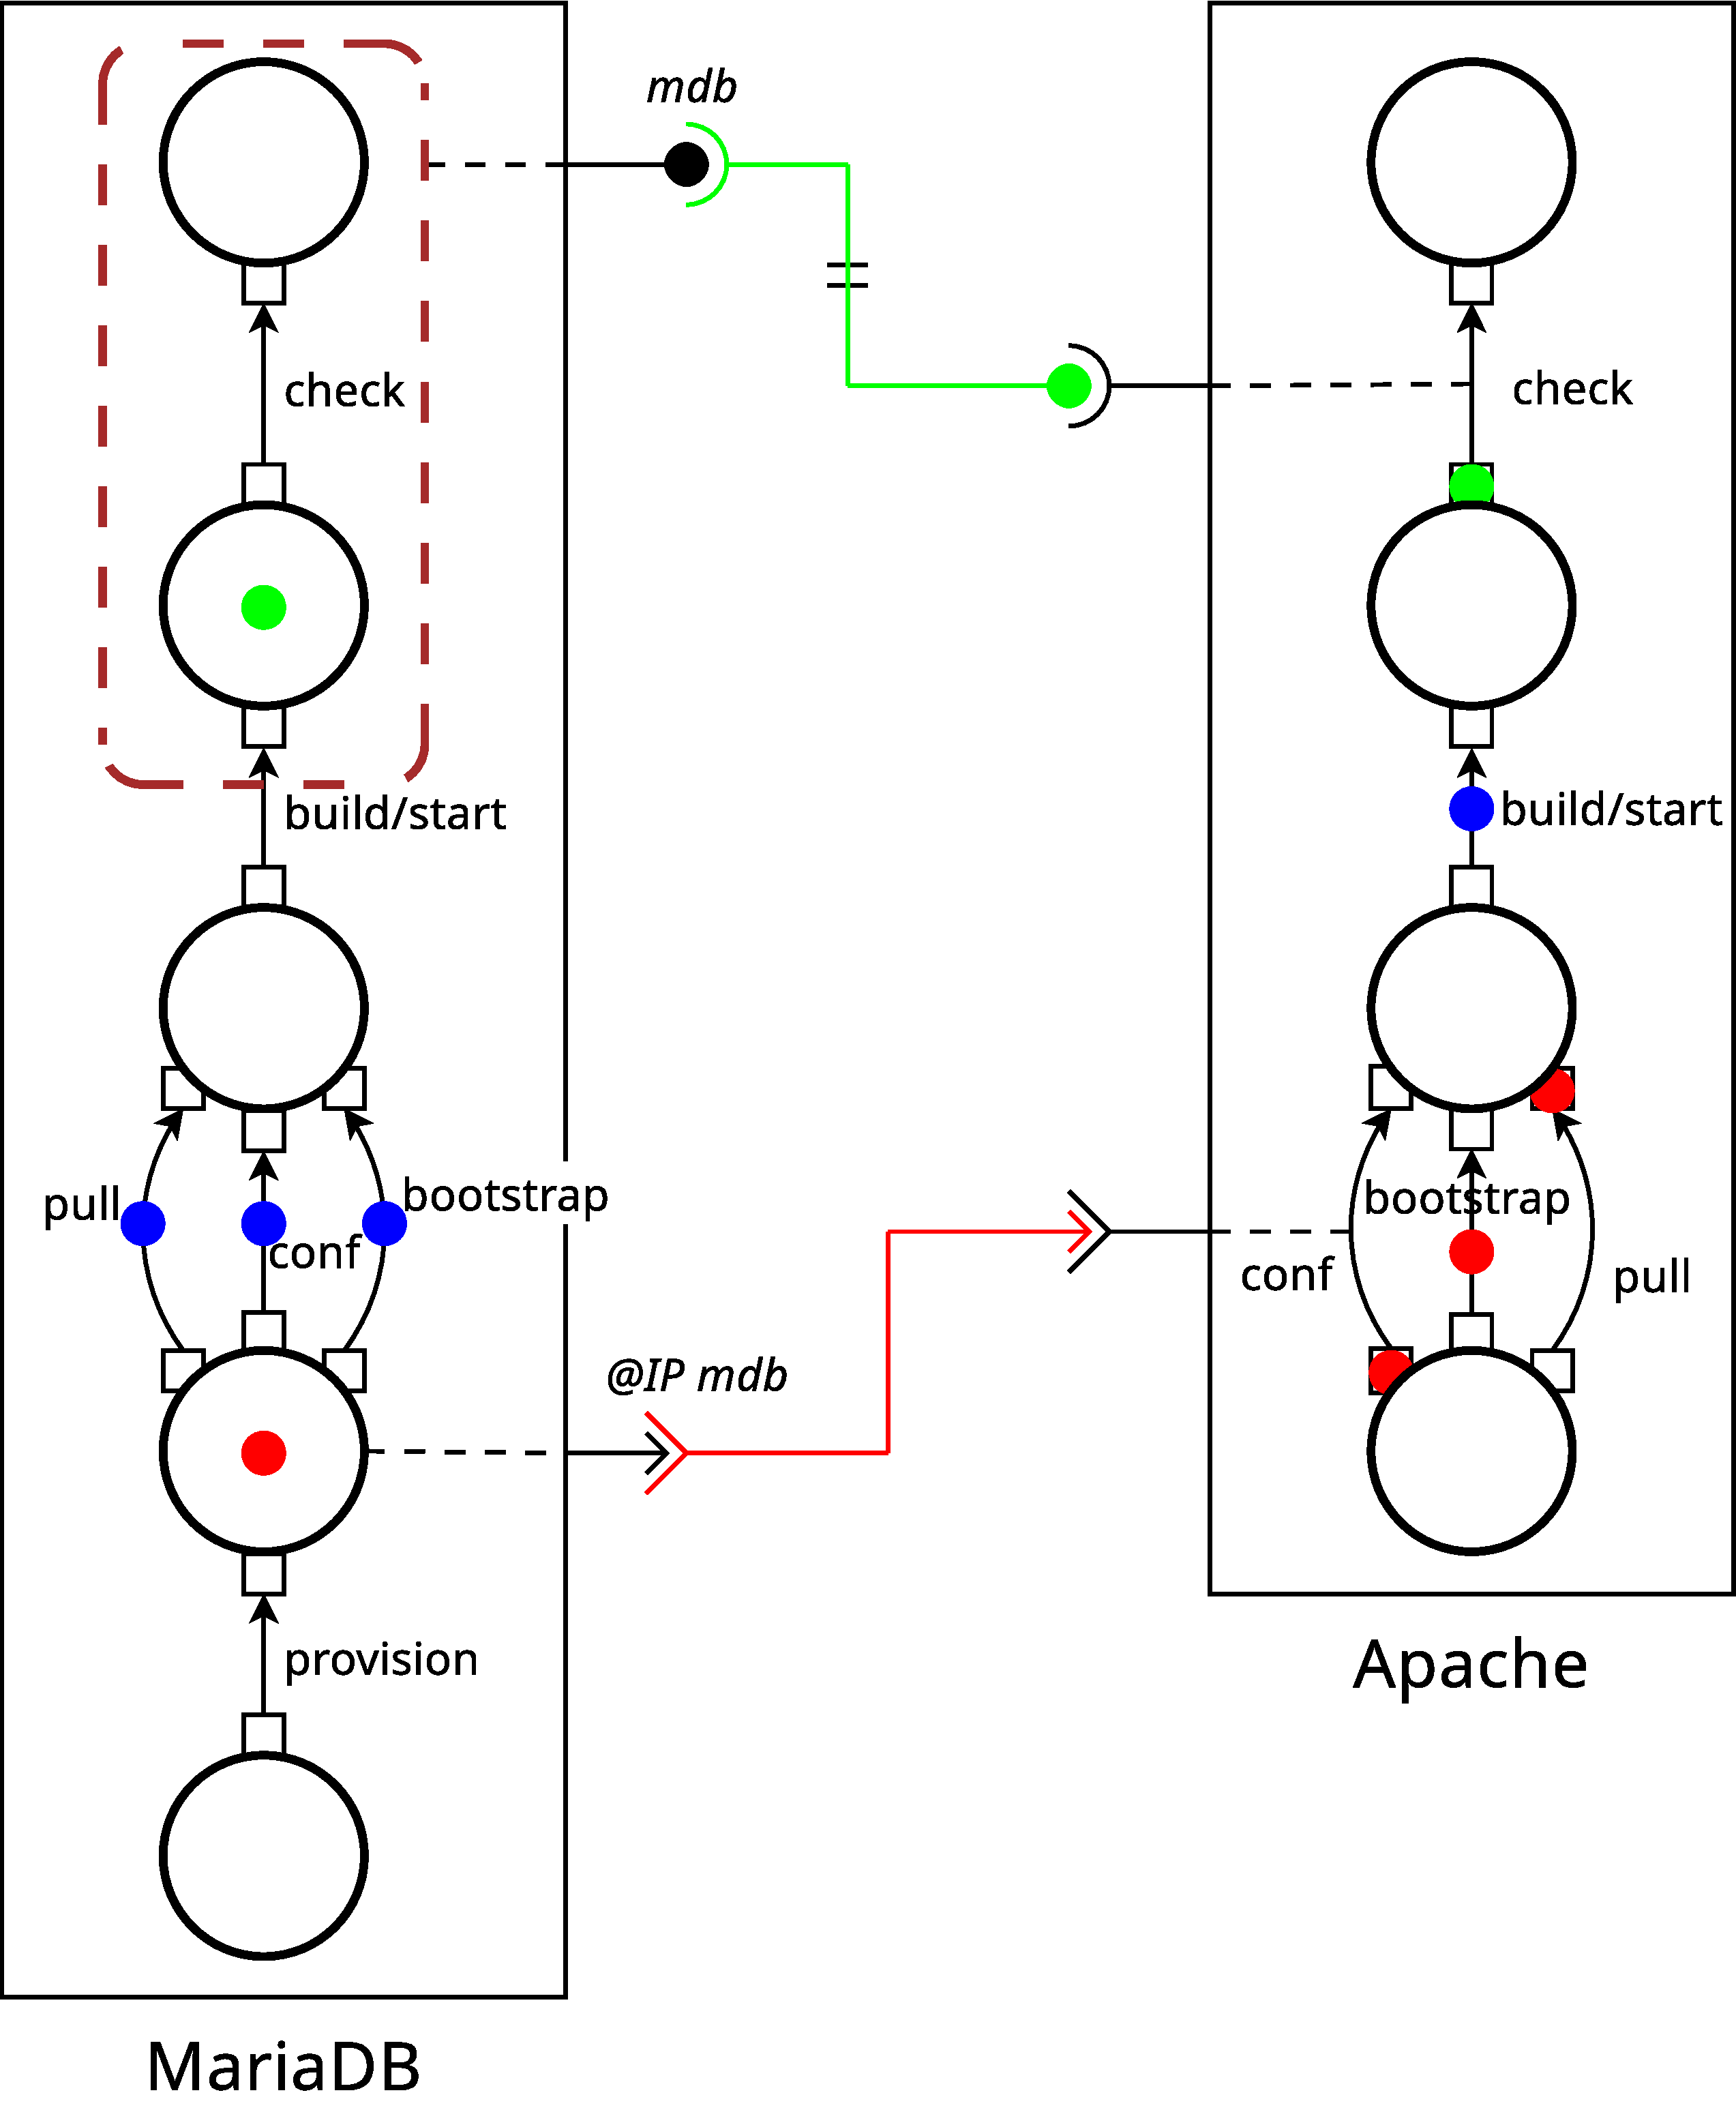
\includegraphics[width=0.7\linewidth]{./images/scenari.pdf}
  \end{center}
  \caption{Three possible intermediate configurations during the commissioning
  of the assembly presented in Figure~\ref{fig:example}. Each configuration is
  represented by a different color.}
  \label{fig:scenari}
\end{figure}

\paragraph{Example}{
Let us detail the commissioning execution of the Apache/MariaDB
example. The initial assembly, given in Figure~\ref{fig:example}, has
already been described. Figure~\ref{fig:scenari} depicts three examples of
configurations that may occur at different steps of the
commissioning. In chronological order, the first configuration is
represented by red tokens, the second one by blue tokens, and the
third one by green tokens.

In the first configuration, on the one hand, the red token of MariaDB
is found on the second place, which can only occur after a token has
been moved from the initial place of the component to the output dock
of transition \texttt{provision} and the action associated with this
transition has been executed. The provide port bound to this place
models data provided by the component, in this case the IP adress
resulting from the action of \texttt{provision}. As soon as this
second place is reached, the provide port \texttt{@IP mdb} is enabled,
and the use port connected to it is provided. On the other hand, the
initial token of Apache has been replaced by three tokens, one for
each output dock. Two of these tokens have been used to fire
respectively the transitions \texttt{bootstrap} and \texttt{pull}, and
\texttt{pull} has terminated. However, the third token has remained in
its dock. The transition \texttt{conf} could not be fired until the
bound use port became provided. In this configuration, this is the
case and the transition may be fired.

The blue configuration illustrates a case where parallel transitions
\texttt{pull}, \texttt{conf}, and \texttt{bootstrap} of MariaDB are
executed simultaneously.

Finally, the green configuration illustrates an example where MariaDB
reaches its penultimate place. The provide port \texttt{mdb} bound to
it models the service offered by the component. As soon as the place
holds a token, the provide port becomes enabled. As a result, the use
port of Apache that is connected to it becomes provided, and the
transition \texttt{check} of Apache can be fired.}


%-------------------------------------------------------
\section{\mad}
\label{sec:forma_model}
%-------------------------------------------------------
%--------------------------
\subsection{Component}
%--------------------------

Formally in \mad, a component is defined as a tuple that can be divided
into four different parts: \emph{places}, \emph{transitions}, \emph{ports} and
\emph{bindings}.

\paragraph{Places}{

A component in \mad is first defined by a set of \emph{places} denoted
$\Pi$. A component is also defined by two sets of
\emph{docks}. A dock is represented by a small square and is attached to a
place. It is used to handle synchronization of parallel branches. The
first set concerns input docks. It is denoted $\Delta_{i}$ and it is
displayed below the place they are attached to. The second set is
denoted $\Delta_{o}$. It contains output docks and is displayed above
the place they are attached to.
The function $place\,:\,\Delta_{o}\cup\Delta_{i}\rightarrow\Pi$
returns the place a dock is attached to. Functions
$dock_i\,:\,\Pi\rightarrow \mathcal{P}(\Delta_{i})$ and
$dock_o\,:\,\Pi\rightarrow \mathcal{P}(\Delta_{o})$ respectively
returns the subset of $\Delta_i$ and $\Delta_o$ attached to a place
$\pi\in\Pi$. Places can be part of one or multiple groups which are
subsets of $\Pi$. The set of groups is denoted $G$. Last, $I \subseteq \Pi$ is the
non-empty set of initial places of the component.

}

\paragraph{Transitions}{

  % -----
\begin{table}[tp]
  \centering
  \resizebox{\columnwidth}{!}{%
    \begin{tabular}{|c|c|}
      \hline
      & \emph{Places}\\
      \hline
      $\Pi$ & set of places of a component\\
      $\Delta_{i}$ & set of input docks of a component\\
      $\Delta_{o}$ & set of output docks of a component\\
      $place$ & function mapping a dock to its place\\
      $dock_{i}$ & function mapping a place to its input docks\\
      $dock_{o}$ & function mapping a place to its output docks\\
      $G$ & set of groups of places\\
      $I$ & subset of places holding a token at initialization\\
      \hline
      \hline
      & \emph{Transitions}\\
      \hline
      $\Theta$ & finite set of transitions\\
      $A$ & finite set of actions\\
      $action$ & function mapping a transition to its corresponding action\\
      $done$ & function indicating if the action of the transition has finished\\
      \hline
      \hline
      & \emph{Ports}\\
      \hline
      $S_{u}$ & set of use ports of a component\\
      $S_{p}$ & set of provide ports\\
      $T_{port}$ & set of types of ports\\
      $type_{p}$ & function mapping a port to its type\\
      $D_{u}$ & set of data use ports of a component\\
      $D_{p}$ & set of data provide ports\\
      $T_{data}$ & set of types of data ports\\
      $type_{d}$ & function mapping a data port to its type\\
      $\mathbb{D}$ & set of possible data values\\
      \hline
      \hline
      & \emph{Bindings}\\
      \hline
      $B_{S_{u}}$ & set of pairs mapping use ports to transitions\\
      $B_{S_{p}}$ & set of pairs mapping provide ports to groups of places\\
      $B_{D_{u}}$ & set of pairs mapping data use ports to transitions\\
      $B_{D_{p}}$ & set of pairs mapping data provide ports to places\\
      \hline
      \hline
      & \emph{Assembly}\\
      \hline
      $C$ & set of component instances of an assembly\\
      $L_S$ & set of use-provide connections of an assembly\\
      $L_D$ & set of data-use-provide connections of an assembly\\
      \hline
      \hline
      & \emph{Semantics}\\
      \hline
      $mk$ & function indicating if an element holds a token\\
      $val_{A,D_p}$ & returns the value given by an action to a data-provide port\\
      $val$ & function mapping a data provide port to its current value\\
      \hline
    \end{tabular}
  }
  \caption{Notations used throughout this paper}
  \label{tab:not}
\end{table}
%-----
A component is also defined by a set of \emph{transitions} denoted
$\Theta$. A transition $\theta \in \Theta$ is a pair containing one
source dock and one destination dock: $\theta =
\left(s,d\right)\,:\,s\in\Delta_{o},\,d\in\Delta_{i}$. 
%\CP{d=i $=>$ i is not defined! $d\in\Delta_i$ tout simplement, non ?}.
%
Each transition is associated to an \emph{action}. The set of actions is
denoted $A$ and the function $action\,:\,\Theta\rightarrow A$ gives the action
associated to a given transition. Finally, the function
$done\,:\,A\rightarrow\mathbb{B}$, where $\mathbb{B}=\left\{
\text{true},\text{false}\right\}$ indicates whether the action of a
transition has finished.
  
}

\paragraph{Ports}{

Places and transitions are internal elements of a \mad component.
The external interfaces of a component in \mad is
composed of \emph{ports}. A component contains a set of \emph{use-ports}
denoted $S_{u}$, and a set of \emph{provide-ports}, denoted
$S_{p}$. Each port is associated to a type in $T_{port}$, and the
function $type_{p}\,:\,S_{u}\cup S_{p}\rightarrow T_{port}$ maps the ports
to their type. 

In addition to traditional use-provide ports of component models,
\mad handles a specific use-provide abstraction for the
transfer of data values. These ports are called \emph{data-use-ports}
and \emph{data-provide-ports}. The set of data-use ports is denoted
$D_{u}$, and the set of data-provide ports is denoted
$D_{p}$. The set of possible data values is denoted
by $\mathbb{D}$. Finally, the function $type_{d}\,:\,D_{u}\cup
D_{p}\rightarrow T_{data}$ returns the data type of a given data port.
  
}

\paragraph{Bindings}{

In a \mad component, places, groups of places and transitions can be
bound to ports through \emph{bindings}. There are four sets of bindings.
First, we denote $B_{S_{u}}$ the set of pairs that maps
each use port to one or multiple internal transitions in $\Theta$, indicating
that these transitions use the service associated to this port: 
$\left(p,\theta\right)\,:\,p\in S_{u},\,\theta\in\Theta$. Second, we
denote $B_{S_{p}}$ the set of pairs that maps each provide port to one or
multiple groups of places, indicating that if at least one token exists in each
group, the port is active: $\left(p,g\right)\,:\,p\in
S_{p},\,g\in G$. Third, we denote $B_{D_{u}}$ the set of pairs that
maps each data use port to one or multiple internal transitions in $\Theta$,
indicating that these transitions use the data associated to this port: 
$\left(d,\theta\right)\,:\,d\in D_{u},\,\theta\in\Theta$. Finally, we
denote $B_{D_{p}}$ the set of pairs that maps each data provide port to
one or multiple places, indicating that the data associated to this port is
available if a token is or has been in one of these places: $\left(d,\pi\right)\,:\,d\in
D_{p},\,\pi\in \Pi$. 
}

%--------------------------
\subsection{Assembly}
%--------------------------

An \emph{assembly} of components represents the instantiation of
components as defined in the previous section, and their connections
through their ports. In \mad an assembly is defined as a triplet
$(C, L_S, L_D)$, where $C$ is a finite set of component instances,
$L_S$ is the set of connections (links) between use ports and
provide ports of compatible types, and $L_D$ is the set of
connections between data-use ports and data-provide ports of
compatible types. For all the components $c_1,\dots,c_n \in C$, we
denote with a star any union of the corresponding sets, for instance
$\Pi^* = \Pi_1 \cup \dots \cup \Pi_n$. We give a similar definition
for functions, for instance
$type_{p}^*\,:\,S_{u}^*\cup S_{p}^*\rightarrow T_{port}$. Connections
are defined as follows:

\begin{itemize}
\item $\left(u,p\right)\ \in L_S,:\,u\in S_{u}^{*},\,p\in S_{p}^{*},\,type_{p}^{*}\left(u\right)=type_{p}^{*}\left(p\right)$,
\item $\left(u,p\right)\ \in L_D,:\,u\in D_{u}^{*},\,p\in D_{p}^{*},\,type_{d}^{*}\left(u\right)=type_{d}^{*}\left(p\right)$.
\end{itemize}

%--------------------------
\subsection{Operational semantics}
\label{subsec:operational_semantics}
%--------------------------

At each moment in the execution of a \mad deployment assembly
$(C, L_S, L_D)$, we define two functions giving the current
status of this assembly. First, the marking function is defined
to evaluate if one element of any component holds a token:
$mk\,:\,\Pi^{*}\cup\Delta_{i}^{*}\cup\Delta_{o}^{*}\cup\Theta^{*}\rightarrow\mathbb{B}$
where $\mathbb{B}=\left\{ \text{true},\text{false}\right\}$. By
construction, an element can either hold one or zero tokens, the
formal proof of this being left as future work.

Second, we define the function
$val\,:\,D_{P}^{*}\rightarrow \mathbb{D}\cup\left\{ \text{null}\right\}$
that returns the current value associated to a data provide port.

We call a \emph{valuation} the tuple $\left\langle mk,val\right\rangle$,
where $mk$ indicates where tokens are locatednand $val$ indicates the
current value of any data provide port.
At initialization the valuation is defined as follows:
\begin{itemize}
\item $mk\left(x\right)=\begin{cases}
\text{true} & \text{if }x\in I^{*}\\
\text{false} & \text{if } x\in\left(\Pi^{*}\setminus I^*\right)\cup\Delta_{i}^{*}\cup\Delta_{o}^{*}\cup\Theta^{*}
\end{cases}$
\item $val\left(d\right)=\text{null}\quad\forall d \in D^*_{p}$
\end{itemize}

\noindent\textbf{Notations.}
\begin{itemize}
  \item For a function $f\,:\,A\rightarrow B$, we denote $f^{\prime}=f\left[a\coloneqq b\right]\,:\,A\rightarrow B$ such that:
    \begin{equation*}
      f^{\prime}\left(x\right)=\begin{cases}
      b & \text{if }x=a\\
      f\left(x\right) & \text{if }x\neq a
      \end{cases}.
    \end{equation*}
  \item We define the function $val_{A,D_p}\,:\,A\times
    D_{P}^*\rightarrow \mathbb{D}$ that returns the data value to assign to a
    given data-provide port after an action.
\end{itemize}

\noindent\textbf{Terminology.}

\begin{figure}[t]
  \begin{center}
    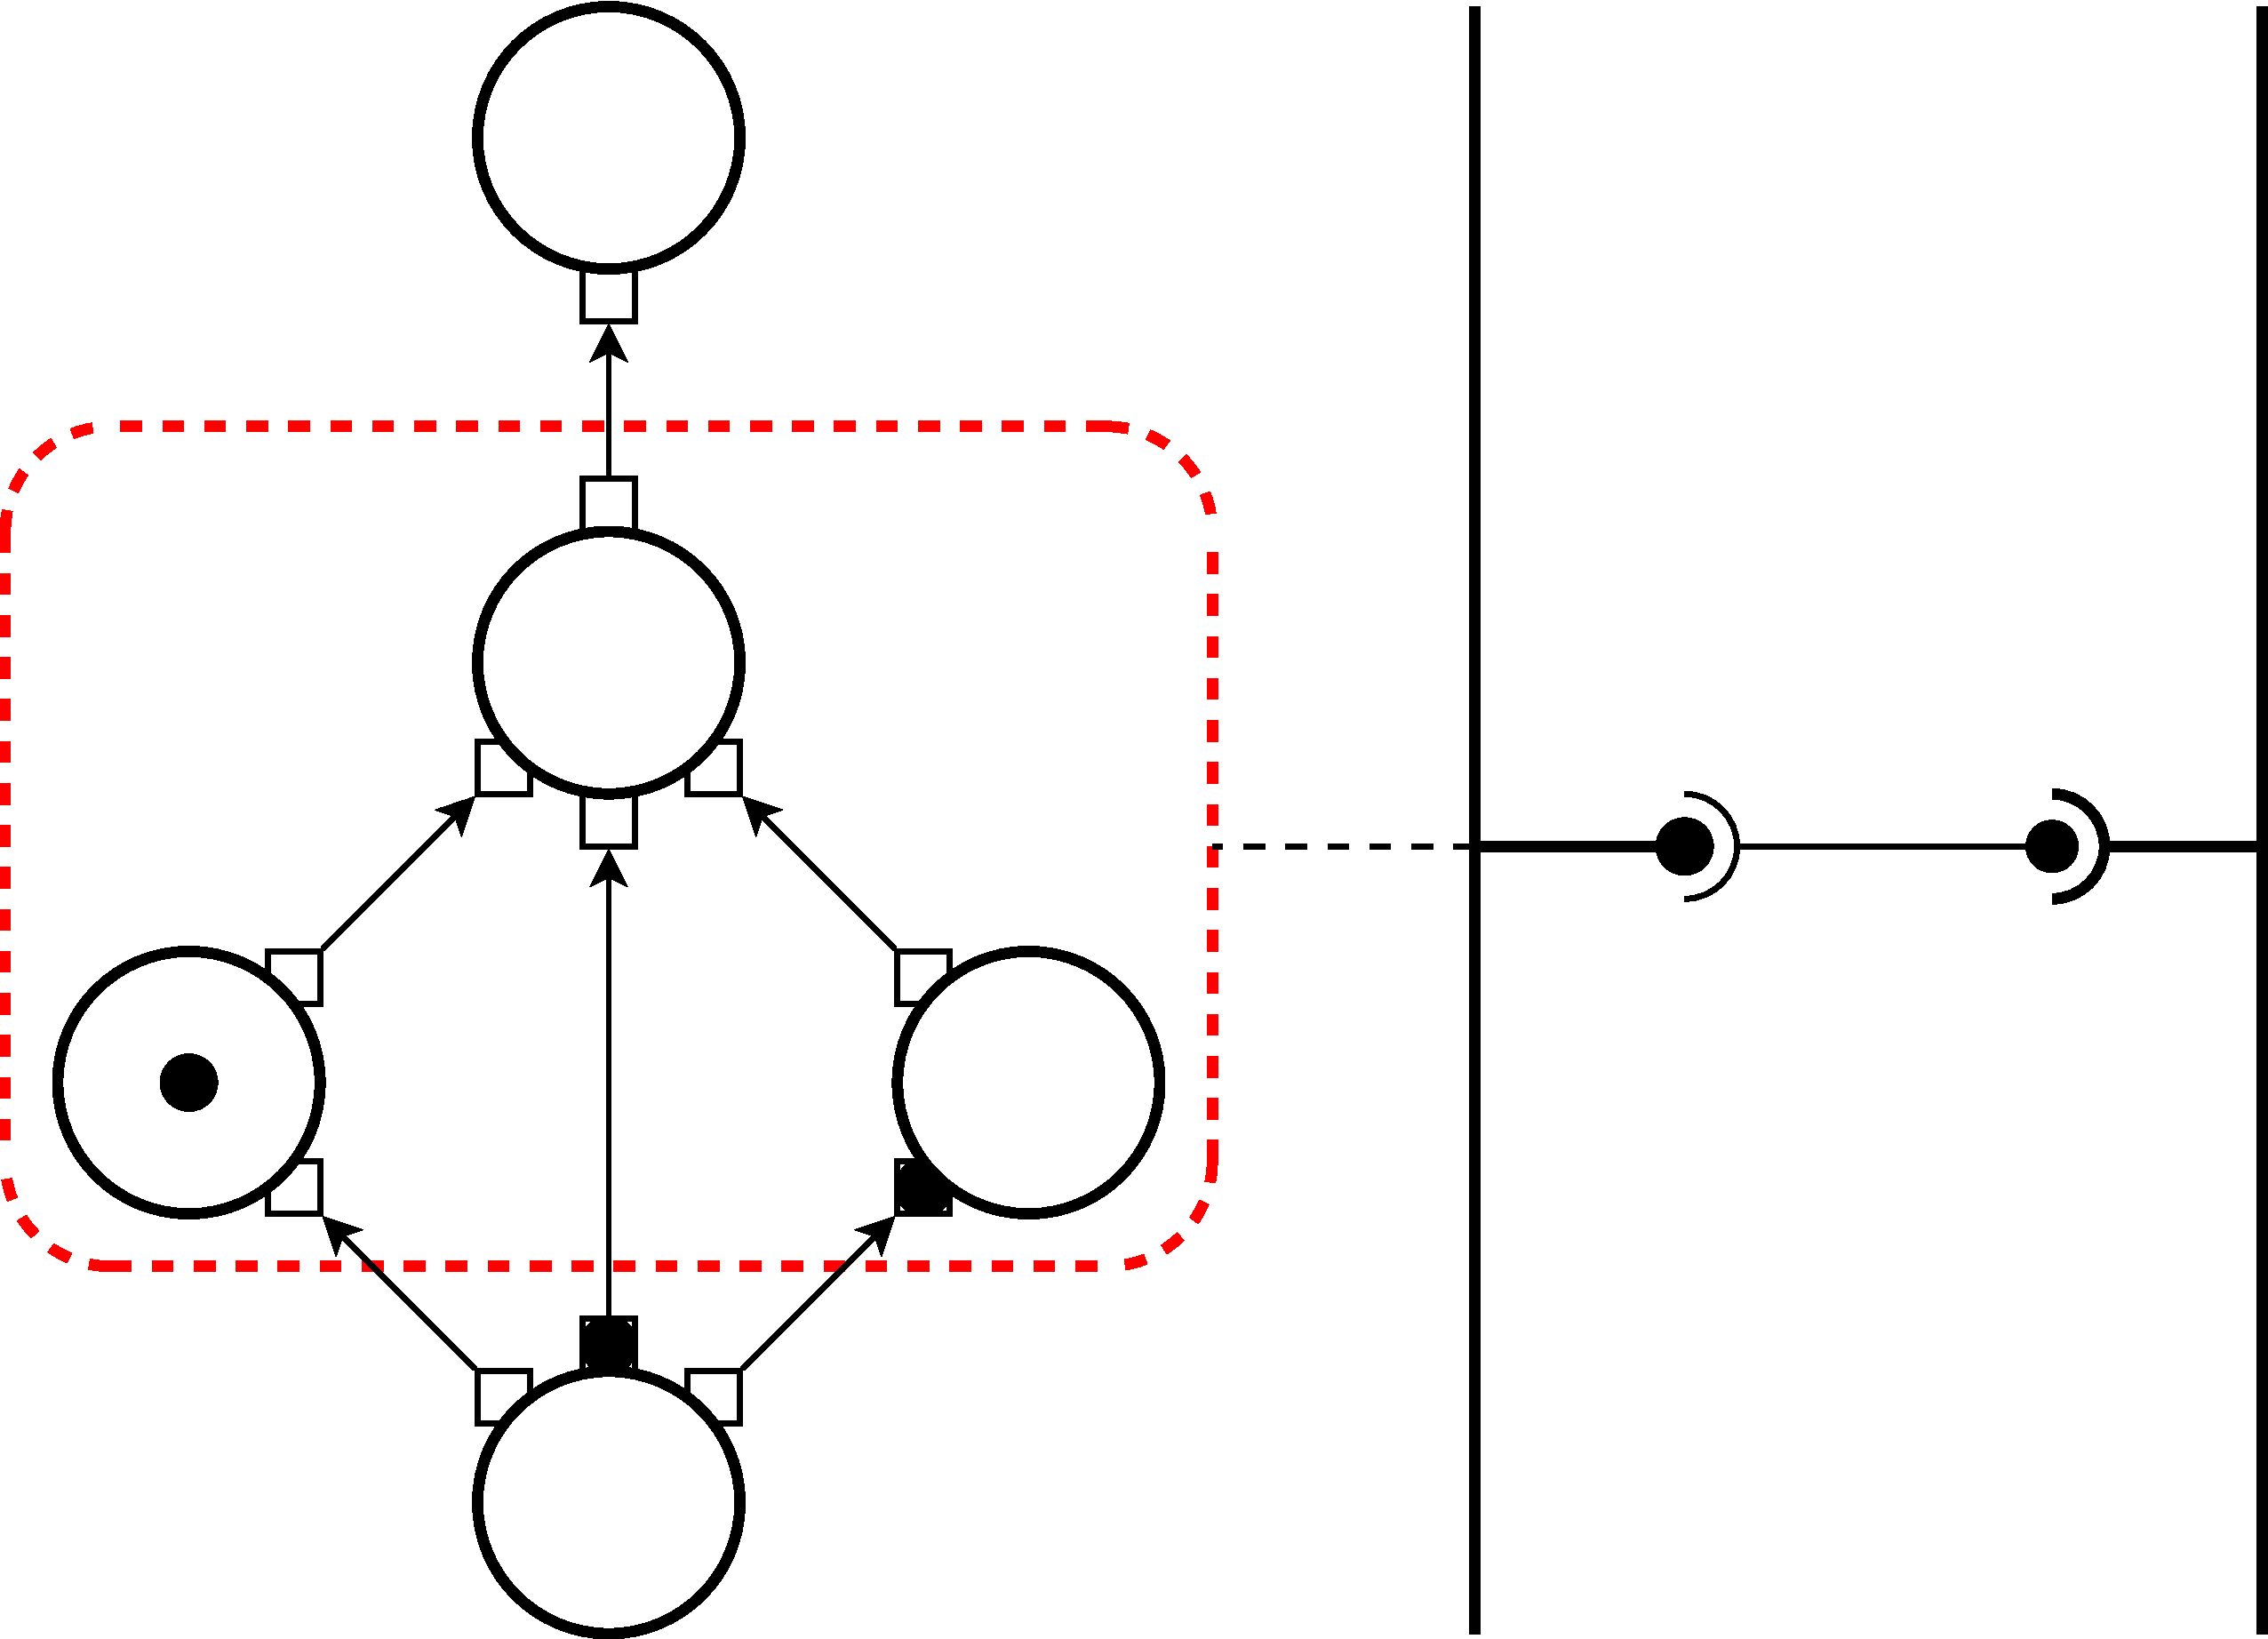
\includegraphics[width=0.7\columnwidth]{./images/enabled_service.pdf}

    \caption{The connection is enabled because its provide port is enabled, as all the groups it is bound to hold a token.}

    \label{fig:enabled_service}
  \end{center}
\end{figure}

\begin{figure}[t]
\begin{center}
  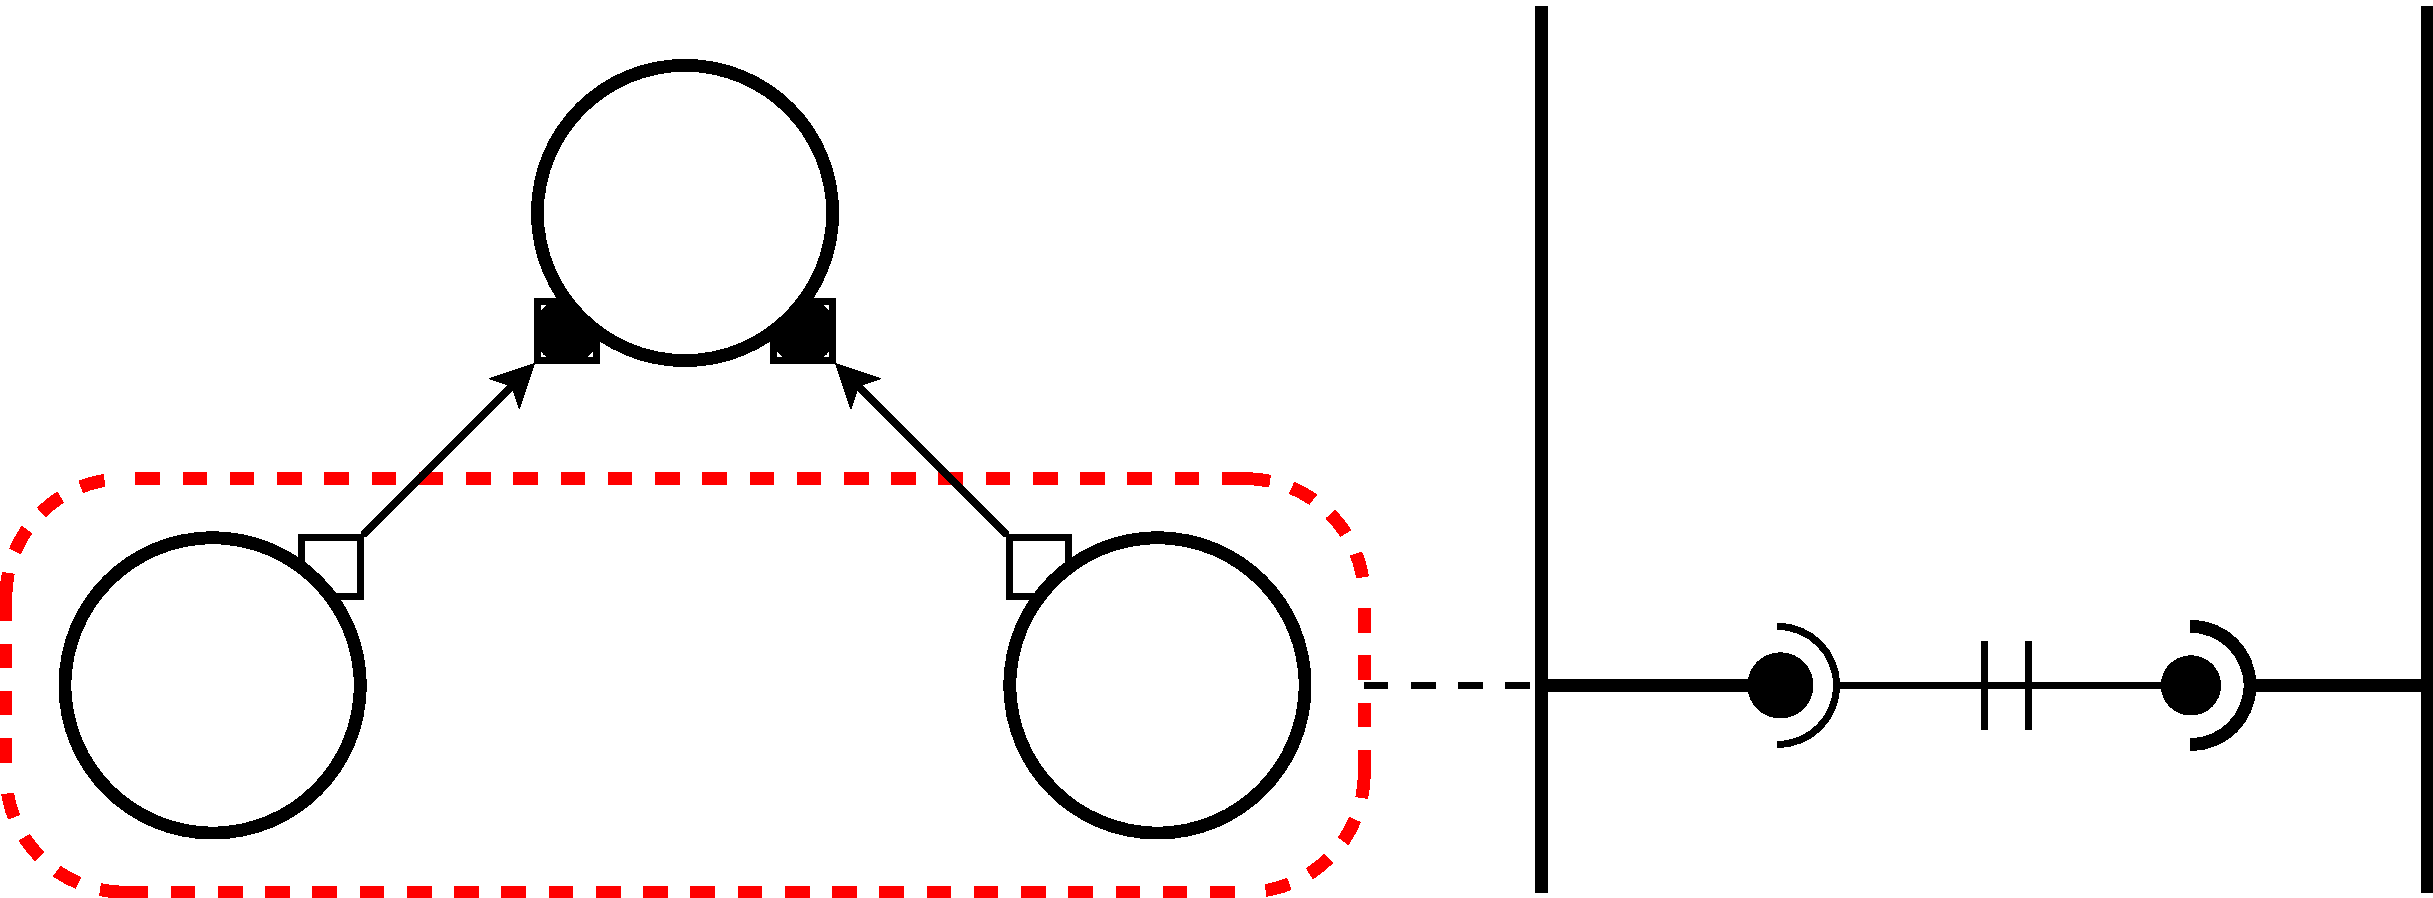
\includegraphics[width=0.7\columnwidth]{./images/disabled_service.pdf}
\end{center}
\caption{The connection is disabled because its provide port is disabled, as one of the groups it is bound to does not hold a token.}
\label{fig:disabled_service}
\end{figure}

\begin{figure}[t]
\begin{center}
  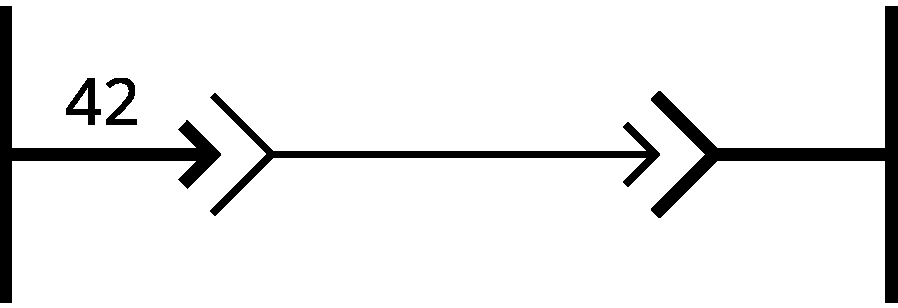
\includegraphics[width=0.4\columnwidth]{./images/enabled_data.pdf}
\end{center}
\caption{The connection is enabled because its data-provide port holds a value.}
\label{fig:enabled_data}
\end{figure}

\begin{figure}[t]
\begin{center}
  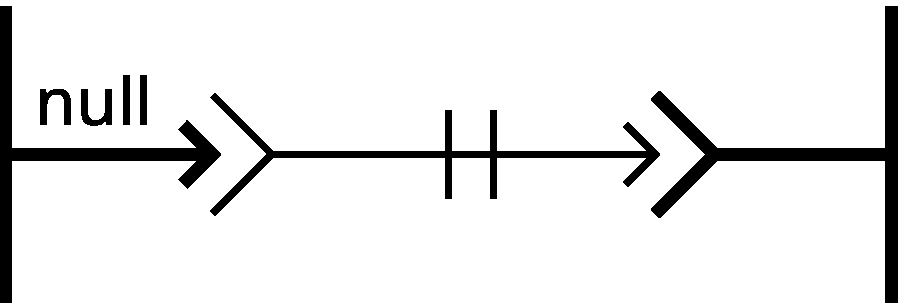
\includegraphics[width=0.4\columnwidth]{./images/disabled_data.pdf}
\end{center}
\caption{The connection is disabled because its data-provide port does not hold a value.}
\label{fig:disabled_data}
\end{figure}




A group is said to be enabled if it contains at least one token (otherwise
it is disabled). A service-provide port is said to be enabled if all the groups it
is bound to are enabled (otherwise it is disabled). A service connection is said to
be enabled if its provide port is enabled (otherwise it is disabled).
Figure~\ref{fig:enabled_service} gives an example of enabled service connection,
while Figure~\ref{fig:disabled_service} gives an example of disabled service connection.

A data-provide port is said to be enabled if it holds a value (otherwise it is disabled).
A data connection is said to be enabled if its provide port is enabled (otherwise it is
disabled).
Figure~\ref{fig:enabled_data} gives an example of enabled data connection,
while Figure~\ref{fig:disabled_data} gives an example of disabled data connection.
    
In this paper, we present four rules to operate the \mad model. We
leave for future work the extension of these rules to support errors
and reconfigurations. The rules are formally defined in
Figure \ref{fig:rules}.

\paragraph{Firing transition}{

The first rule of \mad is formally defined by
Inference rule~(\ref{eq:r1}). The upper part of the rule indicates the
hypotheses needed to fire a transition, \ie starting a transition,
and the lower part indicates the conclusion of the rule, \ie the valuation
changes. To fire a transition, the source dock of the transition
$\theta$ needs a token, and for any port bound to the transition
$\theta$ the connection of this port must be enabled.
The upper part of Figure~\ref{fig:r1} illustrates the
hypotheses and the lower part the conclusion of the rule.

\begin{figure}[t]
\begin{center}
  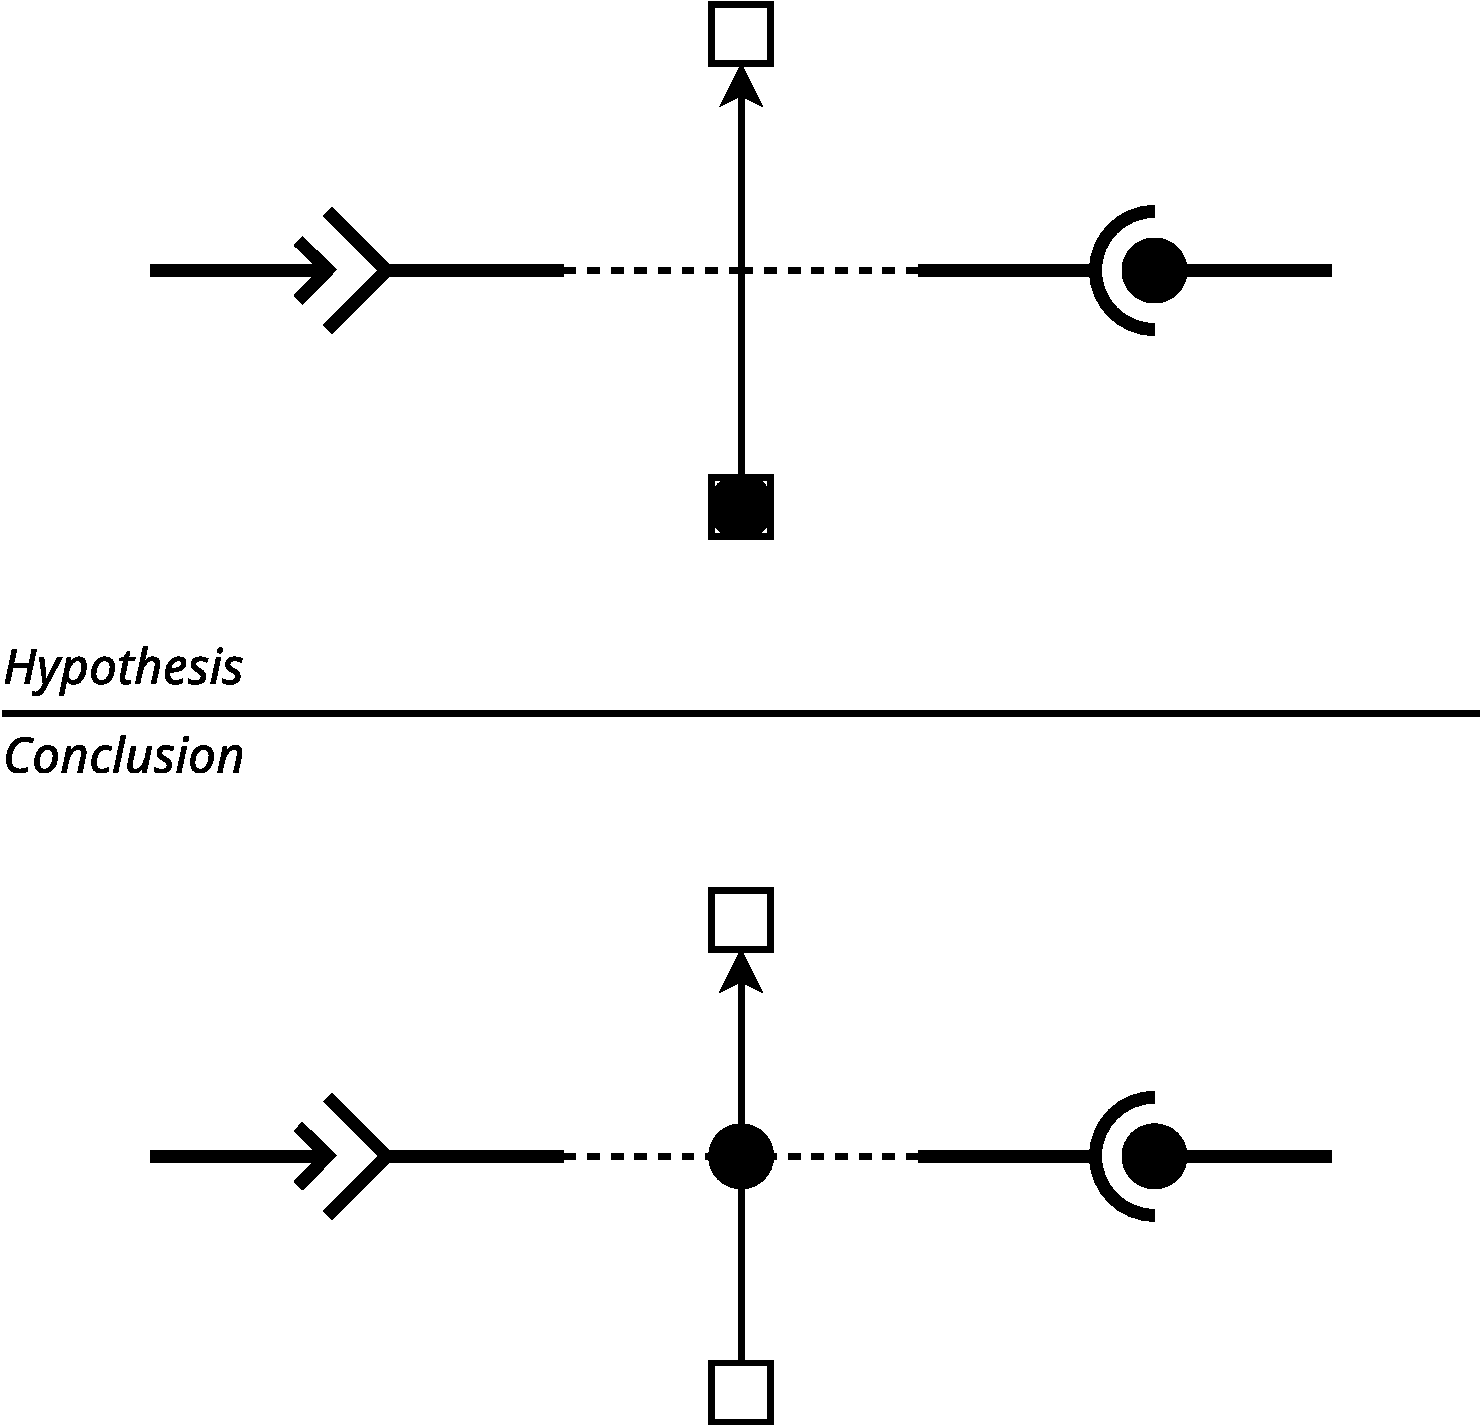
\includegraphics[width=0.55\columnwidth]{./images/firing.pdf}
\end{center}
\caption{Illustration of the rule of Inference rule~(\ref{eq:r1}) to fire transitions.}
\label{fig:r1}
\end{figure}

}

\paragraph{Ending transition}{

The second rule of \mad is formally defined by
Inference rule~(\ref{eq:r2}). To end a transition $\theta$, a token has to
be present on the transition and the action performed by the
transition must be terminated. When ending a transition, the token
is moved from this transition to its destination dock. Note that the ports bound
to the transition cannot be disconnected before applying this rule. Moreover, if
the place to which the destination dock is attached is bound to
data-provide ports, their values are replaced by those computed by the action.
For this reason, the rule uses the function
$val_{A,D_p}$. Figure~\ref{fig:r2} illustrates this rule.
%\MC{Expliquer pourquoi les ports ne peuvent pas etre deconnectes ?}

\begin{figure}[t]
\begin{center}
  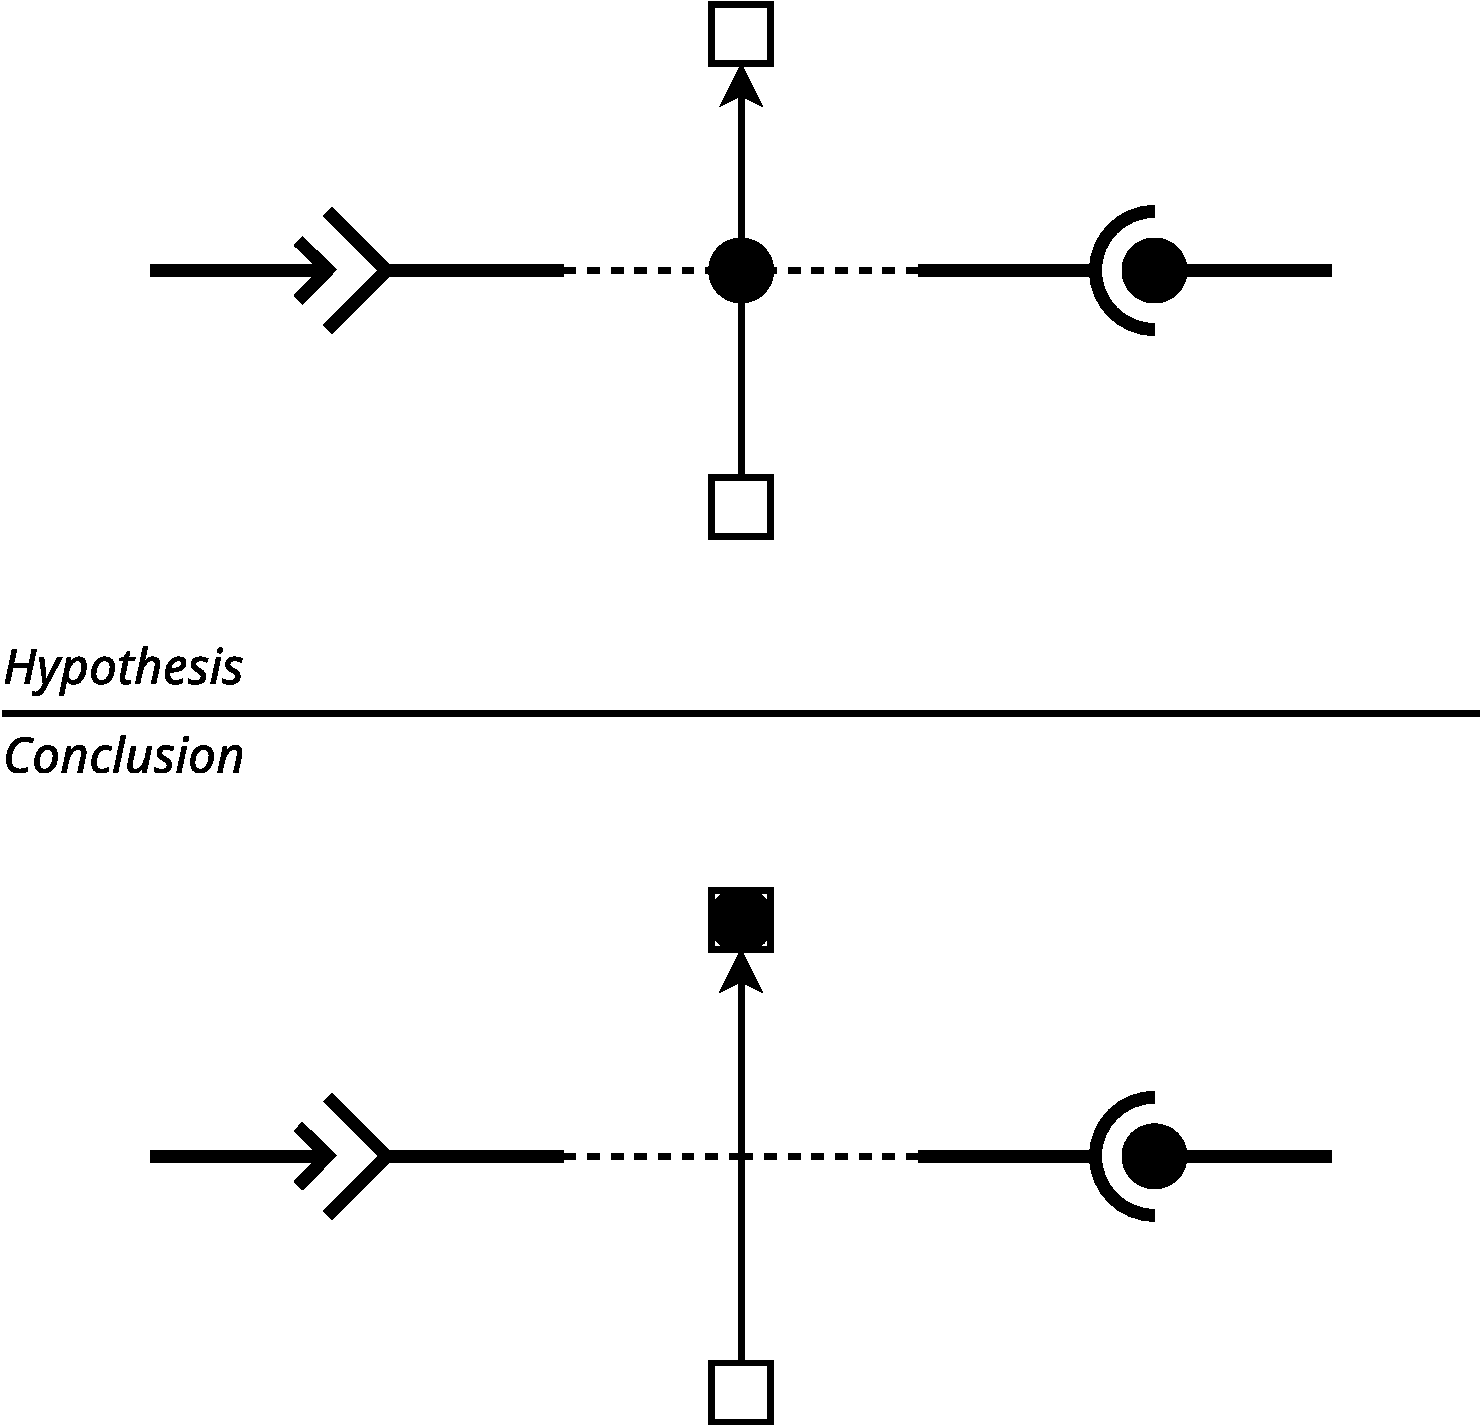
\includegraphics[width=0.55\columnwidth]{./images/ending_transition.pdf}
\end{center}
\caption{Illustration of the rule of Inference rule~(\ref{eq:r2}) to end transitions.}
\label{fig:r2}
\end{figure}
  
}

\paragraph{Input docks to place}{

The third rule of \mad is formally defined by
Inference rule~(\ref{eq:r3}). To move tokens from input docks of a place to
this place, all input docks must hold a token. The conclusion is to remove
all the tokens within the docks and to add one token inside the
place as illustrated in Figure~\ref{fig:r3}.

\begin{figure}[t]

\begin{minipage}[h]{0.45\columnwidth}%
  \centering
  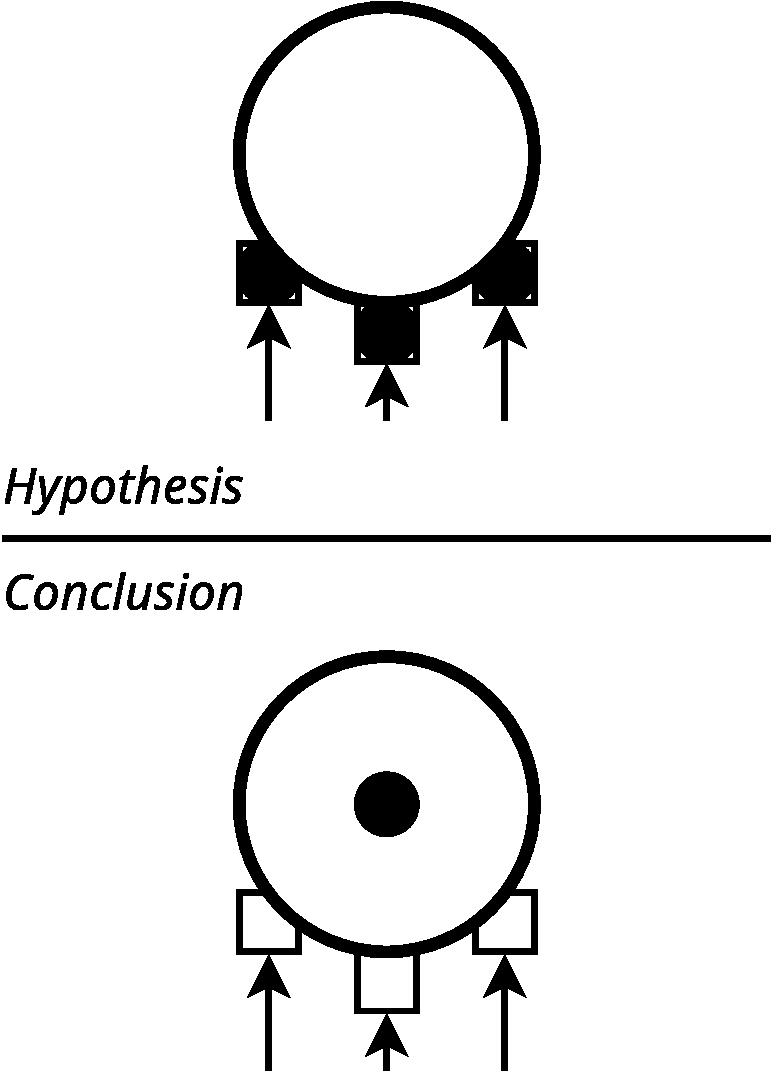
\includegraphics[width=0.65\columnwidth]{./images/inputdocks_to_place.pdf}
  \captionof{figure}{\label{fig:r3}Illustration of the rule of Inference rule~(\ref{eq:r3}) to move tokens from input docks to a place.}
\end{minipage}
\hfill
\begin{minipage}[h]{0.45\columnwidth}%
  \centering
  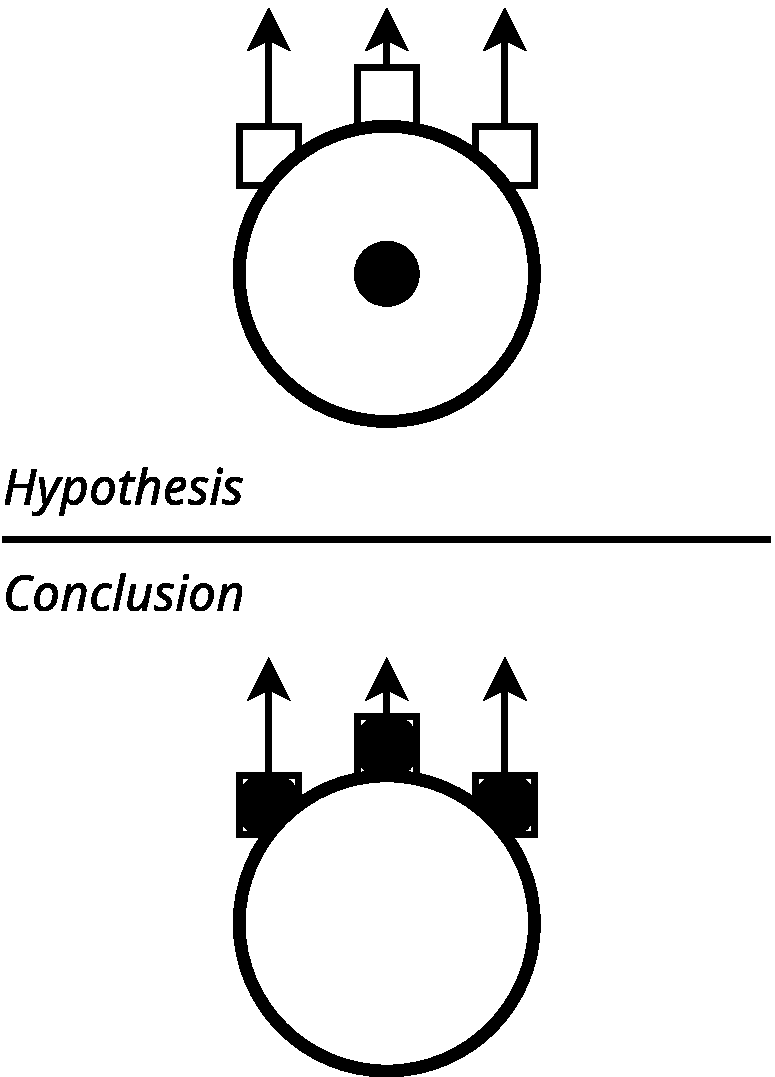
\includegraphics[width=0.65\columnwidth]{./images/place_to_outputdocks.pdf}
  \captionof{figure}{\label{fig:r4}Illustration of the rule of Inference rule~(\ref{eq:r4}) to move tokens from place to output docks.}
\end{minipage}
\end{figure}

\paragraph{Place to output docks}{

The fourth rule of \mad is formally defined by
Inference rule~(\ref{eq:r4}). To move a token from a place to its output
docks, a token needs to be present onto the place. Also, if the place
is part of a group which is itself bound to a used provide port,
applying the rule must not make the last token of the group leave,
otherwise this provide port becomes inactive. A provide port is said
to be used if it is connected to a use port bound to a transition
holding a token.  If these conditions are met, the token can be
removed from the place, and a token is added onto each output dock
attached to this place. This rule is illustrated in
Figure~\ref{fig:r4} in a simplified manner.

}

%------------
\begin{figure*}[tp]
%
\begin{equation}
\cfrac{\theta =\left(s,d\right) \in \Theta^*,s \in \Delta_o^*,d \in \Delta_i^*\qquad mk\left(s\right)\qquad\forall p \in S_{u}\cup D_{u},\left(p,\theta\right)\in B_{S_{u}}^{*}\cup B_{D_{U}}^{*}\,:\,\text{is\_ready}(p)}{\left\langle mk,val\right\rangle \rightarrow\left\langle mk\left[s\coloneqq\text{false}\right]\left[\theta\coloneqq\text{true}\right],val\right\rangle }
\label{eq:r1}
\end{equation}
%
\begin{align*}
  \text{where: }\text{is\_ready}(p) = &\, \exists u\in S_u\cup D_u,\,(u,p)\in L_{S}\cup L_D\land \text{is\_conn\_enabled}\left((u,p)\right) \\
  \text{is\_conn\_enabled}\left((u,p)\right) = &\, \begin{cases}
\forall g\in G,\left(p,g\right)\in B_{S_{p}}\,:\,\text{is\_group\_enabled}\left(g,mk\right) & \text{if }\left(u,p\right)\in L_{S}\\
val\left(p\right)\neq\text{null} & \text{if }\left(u,p\right)\in L_D
\end{cases} \\
\text{is\_group\_enabled}\left(g,mk\right) = & \left(\exists\,\pi\in g:\,mk\left(\pi\right)\right)\\
 & \, \lor\left(\exists\,\delta\in\Delta_{o}^{*}\cup\Delta_{i}^{*}:\,mk\left(\delta\right)\land \left(\exists(s,d)\in\Theta^{*}:\,\left(\delta=s\lor \delta=d\right)\land \text{is\_in\_group}\left((s,d),g\right)\right)\right)\\
 & \, \lor\left(\exists\,\theta\in\Theta^{*}:\,mk\left(\theta\right)\land \text{is\_in\_group}\left(\theta,g\right)\right) \\
\text{is\_in\_group}\left((s,d),g\right) = & place\left(s\right)\in g\land place\left(d\right)\in g
\end{align*}
%
\begin{equation}
\cfrac{\theta=\left(s,d\right) \in \Theta^*\qquad mk\left(\theta\right)\qquad done\left(action\left(\theta\right)\right)}{\left\langle mk,val\right\rangle \rightarrow\left\langle mk\left[\theta\coloneqq\text{false}\right]\left[d\coloneqq\text{true}\right],val\left[\forall p\in D_P^*,\text{dest}(p)\,:\, p\coloneqq val_{A,D_p}(action(\theta),p)\right]\right\rangle}
\label{eq:r2}
\end{equation}
%
\begin{equation*}
  \text{where: }\text{dest}(p) = \left(p,g\right)\in B_{D_{p}}^*,place(d)\in g
\end{equation*}
%
\begin{equation}
\cfrac{\pi\in\Pi^*\qquad D_i=dock_i(\pi)\qquad\forall\delta\in D_i\,mk\left(\delta\right)}{\left\langle mk,val\right\rangle \rightarrow\left\langle mk\left[\forall\delta\in D_i\,:\,\delta\coloneqq\text{false}\right]\left[\pi\coloneqq\text{true}\right],val\right\rangle }
\label{eq:r3}
\end{equation}
%
\begin{equation}
\cfrac{\pi\in\Pi^{*}\qquad D_o=dock_o(\pi)\qquad mk\left(\pi\right)\qquad \forall g\in G,\pi\in g:\,\text{can\_leave}\left(\pi,D_o,g\right)}{\left\langle mk,val\right\rangle \rightarrow\left\langle mk\left[\forall\delta\in D_o\,:\,\delta\coloneqq\text{true}\right]\left[\pi\coloneqq\text{false}\right],val\right\rangle }
\label{eq:r4}
\end{equation}
%
\begin{align*}
\text{where: }\text{can\_leave}\left(\pi,D_o,g\right) = & \left(\exists p,(p,g)\in B_{S_p}:\,\text{is\_used}(p)\right)\implies \lnot \text{last\_token\_leaves} \left(\pi,D_o,g\right) \\
\text{is\_used}\left(p\right) = & \exists u\in S_{u}^{*},\theta\in\Theta^{*}:~\left(p,u\right)\in L_S\land \left(u,\theta\right)\in B_{S_u}^{*}\land mk\left(\theta\right) \\
\text{last\_token\_leaves}\left(\pi,D_o,g\right) = & \left(\text{is\_group\_enabled}\left(g,mk\right)\land\lnot \text{is\_group\_enabled} \left(g,mk\left[\pi\coloneqq \text{false}\right]\left[\forall d\in D_o \,:\,d\coloneqq \text{true}\right]\right)\right) \\
\end{align*}
%
\caption{The four operational semantics rules of \mad.}
\label{fig:rules}
\end{figure*}
%------------

%--------------------------
%\subsection{Consistency rule}
%--------------------------
\textbf{Consistency.}

In \mad, the maximum number of tokens that can be used is the number
of possible parallel branches. A token can only be created during a
branching (rule \emph{place to output docks}), where one token is
created for each output dock of the place. For this reason, cycles are
forbidden in \mad, otherwise an infinity of tokens could be created
which does not make sense within a deployment. We plan in future work
on reconfiguration to allow cycles in very specific settings to keep
control on the tokens and their creation.

\HC[All]{Maybe the performance model in this section too if short
  enough}


%-------------------------------------------------------
\section{Performance model}
\label{sec:perf_model}
%-------------------------------------------------------
In this section, we present \mad' performance model. Its goal is,
given a \mad assembly to be executed and the execution time of all the
transitions of all the components in an assembly, to estimate the total
execution time of the commissionning.
%
Intuitively, we automatically model the execution flow of a \mad
assembly based on \mad' formal semantics. This is done by generating a
dependency graph representing the execution flow of each \mad
component in the assembly and connecting them together according to their
dependencies (the connections between their ports). Then, a
\emph{source} vertex is connected to the vertices representing the beginning of
the execution of each component, and a \emph{sink} vertex is created to which
are connected the vertices representing the end of the execution of each
component.
%
Thus, a dependency graph representing the execution of the whole
assembly is obtained. By weighting the arcs corresponding to the transitions with
these transitions' individual execution time (and the other ones with 0),
we can find the total execution time of the assembly by finding the longest
path from the \emph{source} vertex to the \emph{sink} vertex.

% By generating a graph modelling the execution flow of a \mad assembly,
% capturing both intra-component and inter-component dependencies, we
% reduce this problem to finding the longest path in a DAG.

\subsection{Notations}

Recall that given a component, we denote its set of places $\Pi$ and its
set of transitions $\Theta$. In the following, we consider that the
transitions go directly from a place to
another place instead of from an output dock to an input dock.
Hence, $\Theta$ is a multiset which elements are pairs of places. We
can obtain the place corresponding to each dock by using the $place$
function of the component.

In order to estimate the total commissionning time, we need to know the
execution time of each individual transition. In the following, we
consider the function $time\,:\,\Theta\rightarrow\mathbb{R}^{+}$
associating an execution time to each transition (taken as input).

We also consider the following two functions:
\MC[Maverick]{Change group entrance and exit functions to return only one element?
State that we consider only the assemblies in which these functions always return
one element?}
\begin{itemize}
\item the \emph{group entrance function} $g_{in}\,:\,G\rightarrow\mathcal{P}\left(\Pi\right)$ with\\
$g_{in}(g)=\left\{ \pi\,\mid\,\pi\in g\land\exists\pi_{b}\,:\,\left(\pi_{b}\not\in g\land\left(\pi_{b},\pi\right)\in\Theta\right)\right\} $
(the result of $g_{in}$ is called the set of \emph{entrance places}
of the group)
\item the \emph{group exit function} $g_{out}\,:\,G\rightarrow\mathcal{P}\left(\Pi\right)$ with\\
$g_{out}(g)=\left\{ \pi\,\mid\,\pi\in g\land\exists\pi_{a}\,:\,\left(\pi_{a}\not\in g\land\left(\pi,\pi_{a}\right)\in\Theta\right)\right\} $
(the result of $g_{out}$ is called the set of \emph{exit places}
of the group)
\end{itemize}

Recall that an assembly is a tuple $\left(C,L_{P},L_{D},ebl\right)$. In
the following, we consider that
$C=\bigcup_{i=1}^{n}\left\{ \left(\Pi_{i}\dots,\left(B_{D_{p}}\right)_{i}\right)\right\} $.
For each notation $X$ specific to a component, we denote $X_{all}$ the
union (in the case of an assembly) or the extension (in the case of
a function) for all components. For instance:
\begin{itemize}
\item $\Pi_{all}=\bigcup_{i=1}^{n}\Pi_{i}$ (set of all \emph{places} in
the assembly)
\item $\left(time\right)_{all}\,:\,\Theta_{all}\rightarrow\mathbb{R}^{+}$
(function giving the \emph{execution time} of each transition) with:
$\left(time\right)_{all}\left(x\right)=\left(time\right)_{i}\left(x\right)$
if $x\in\Theta_{i}$ 
\end{itemize}
The execution flow graph is an oriented weighted graph \emph{$\left(V,A\right)$}
where $V$ is the set of vertices and $A$ is the multiset of weighted
arcs with elements in $V\times V\times\mathbb{R}^{+}$. We define
$V$ and $A$ in the following.

\subsection{Vertices}

For each place, we associate two vertices: one representing the place
itself and one representing the event of a token leaving the place.
Figure~\ref{fig:place_graph} depicts the transformation of one place
\emph{running} to a dependency graph.
\[
V_{\Pi}=\bigcup_{\pi\in\Pi_{all}}\left\{ v_\pi^\text{place},v_\pi^\text{leaving}\right\} 
\]

For each transition, we associate two vertices: one representing the
beginning of the transition and one representing its end.
Figure~\ref{fig:transition_graph} depicts the transformation of three
transitions \emph{t1}, \emph{t2} and \emph{t3} to a dependency graph.
\[
V_{\Theta}=\bigcup_{\theta\in\Theta_{all}}\left\{ v_\theta^\text{beginning},v_\theta^\text{end}\right\} 
\]

For each data (use or provide) port we associate one vertex representing
its activation.
Figure~\ref{fig:data_ports_graph} depicts the transformation of one
data provide port \emph{dp} and one data use port \emph{du}.
\[
V_{data}=\bigcup_{u\in\left(D_{u}\right)_{all}\cup\left(D_{p}\right)_{all}}\left\{ v_u^\text{start}\right\} 
\]

For each service (use or provide) port we associate two vertices:
one representing its activation and one its deactivation.
Figure~\ref{fig:service_ports_graph} depicts the transformation of one
service provide port \emph{dp} and one service use port \emph{du}.
\[
V_{service}=\bigcup_{p\in\left(P_{u}\right)_{all}\cup\left(P_{p}\right)_{all}}\left\{v_p^\text{start},v_p^\text{stop}\right\} 
\]

Finally, we define $V$ as the union of all these, plus one source
and one sink vertices. 
\[
V=V_{\Pi}\cup V_{\Theta}\cup V_{data}\cup V_{service}\cup\left\{ v^\text{source},v^\text{sink}\right\} 
\]


\subsection{Arcs}

In the dependency graph, arcs represent time constraints: the event represented
by the destination vertex must happen after the one represented by the source
vertex, at least $w$ seconds apart where $w$ is the weight of the arc. In
practice, the weight of all of the arcs except those corresponding to the
transitions is 0. The weights of the latter are the execution times of the
transitions.

For each place $\pi$ we associate one arc going from $v_\pi^\text{place}$ to
$v_\pi^\text{leaving}$. This represents the fact that a token may leave $\pi$
only after it has entered it.
Figure~\ref{fig:place_graph} depicts the transformation of one place
\emph{running} to a dependency graph.
\[
A_{\Pi}=\bigcup_{\pi\in\Pi_{all}}\left\{ \left(v_\pi^\text{place},v_\pi^\text{leaving},0\right)\right\} 
\]

\begin{figure}[h]
  \subfloat[Concerto assembly]{%
    \begin{minipage}[c]{0.5\columnwidth}%
      \centering
      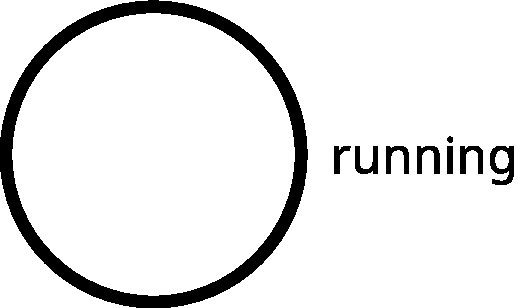
\includegraphics[scale=0.2]{images/perf_place.pdf}
    \end{minipage}
  }
  \subfloat[Dependency graph]{%
    \begin{minipage}[c]{0.5\columnwidth}%
      \centering
      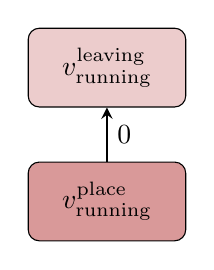
\begin{tikzpicture}[node distance=1.7cm]
        \node (leaving) [leaving] {$v_\text{running}^\text{leaving}$};
        \node (place) [place, below of=leaving] {$v_\text{running}^\text{place}$};
        \draw [arrow] (place) -- (leaving) node[midway, right] {$0$};
      \end{tikzpicture}
    \end{minipage}
  }
  \caption{Vertices and arcs for a place}
  \label{fig:place_graph}
\end{figure}

For each transition $\theta$ going from $\pi_s$ to $\pi_d$, we associate
three arcs. The first between $v_\theta^\text{beginning}$ and $v_\theta^\text{end}$
represents the fact that the end of $\theta$ happens at the time of the
start of $\theta$ plus its duration. The second between $v_{\pi_{s}}^\text{leaving}$
and $v_\theta^\text{beginning}$ represents the fact that $\theta$ may only
happen after a token leaved $\pi_s$. The third one between $v_\theta^\text{end}$ and
$v_{\pi_{d}}^\text{place}$ represents the fact that a token may enter $\pi_d$ only
after $\theta$ has finished.
Figure~\ref{fig:transition_graph} depicts the transformation of three
transitions \emph{t1}, \emph{t2} and \emph{t3} to a dependency graph.
\begin{align*}
A_{\Theta}=\bigcup_{\theta=\left(\pi_{s},\pi_{d}\right)\in\Theta_{all}} & \left\{ \left(v_\theta^\text{beginning},v_\theta^\text{end},time_{all}\left(\theta\right)\right),\right.\\
 & \left(v_{\pi_{s}}^\text{leaving},v_\theta^\text{beginning},0\right),\\
 & \left. \left(v_\theta^\text{end},v_{\pi_{d}}^\text{place},0\right)\right\}
\end{align*}

\begin{figure*}[h]
  \subfloat[Concerto assembly]{%
    \begin{minipage}[c]{0.8\columnwidth}%
      \centering
      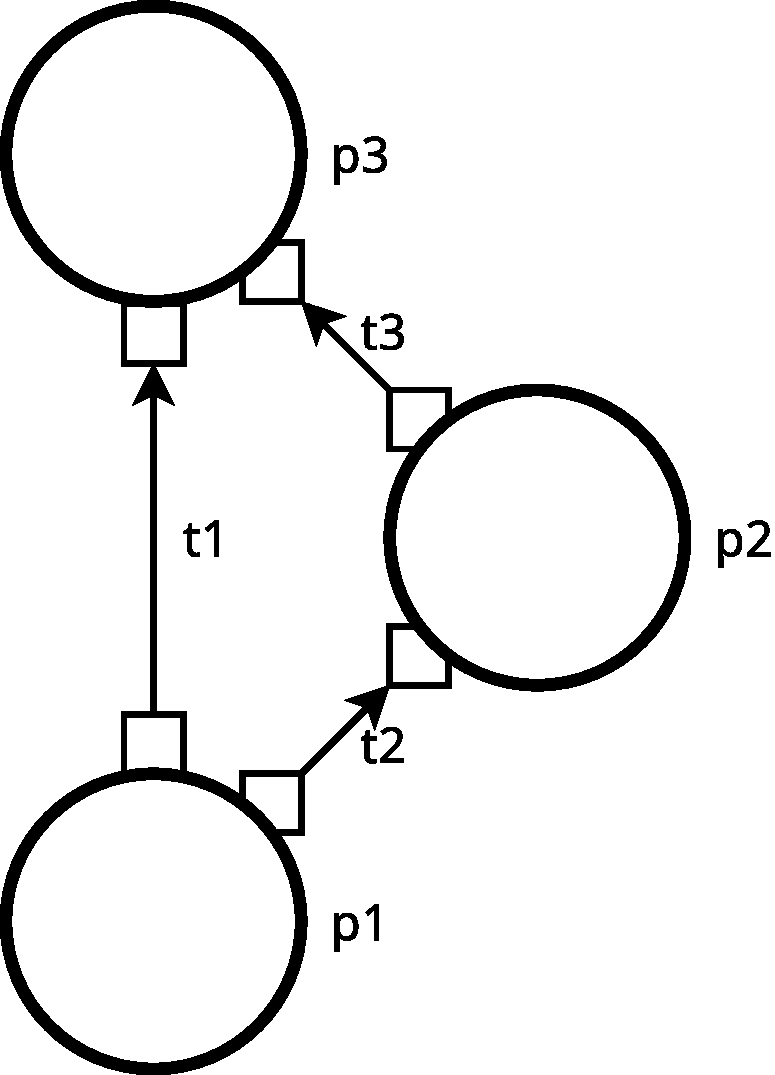
\includegraphics[scale=0.2]{images/perf_transition.pdf}
    \end{minipage}
  }
  \hfill
  \subfloat[Dependency graph]{%
    \begin{minipage}[c]{1.2\columnwidth}%
      \centering
      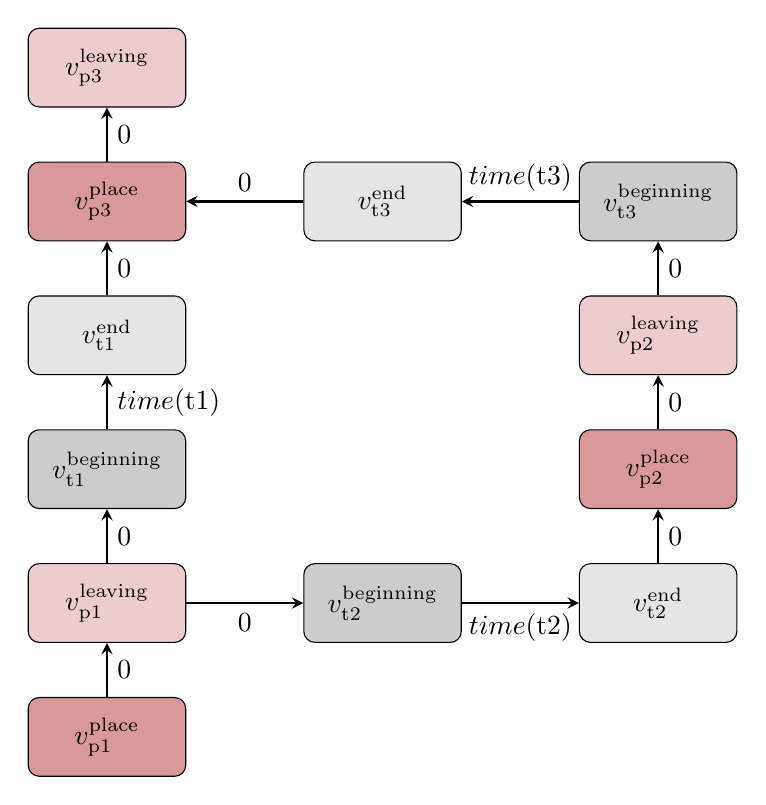
\begin{tikzpicture}[node distance=1.7cm]
        \node (p3l) [leaving] {$v_\text{p3}^\text{leaving}$};
        \node (p3) [place, below of=p3l] {$v_\text{p3}^\text{place}$};
        \node (t1e) [end, below of=p3] {$v_\text{t1}^\text{end}$};
        \node (t1) [beginning, below of=t1e] {$v_\text{t1}^\text{beginning}$};
        \node (p1l) [leaving, below of=t1] {$v_\text{p1}^\text{leaving}$};
        \node (p1) [place, below of=p1l] {$v_\text{p1}^\text{place}$};
        \node (t2) [beginning, right of=p1l, xshift=1.8cm] {$v_\text{t2}^\text{beginning}$};
        \node (t2e) [end, right of=t2, xshift=1.8cm] {$v_\text{t2}^\text{end}$};
        \node (p2) [place, above of=t2e] {$v_\text{p2}^\text{place}$};
        \node (p2l) [leaving, above of=p2] {$v_\text{p2}^\text{leaving}$};
        \node (t3) [beginning, above of=p2l] {$v_\text{t3}^\text{beginning}$};
        \node (t3e) [end, right of=p3, xshift=1.8cm] {$v_\text{t3}^\text{end}$};
        \draw [arrow] (p3) -- (p3l) node[midway, right] {$0$};
        \draw [arrow] (p2) -- (p2l) node[midway, right] {$0$};
        \draw [arrow] (p1) -- (p1l) node[midway, right] {$0$};
        \draw [arrow] (t3) -- (t3e) node[midway, above] {$time(\text{t3})$};
        \draw [arrow] (t2) -- (t2e) node[midway, below] {$time(\text{t2})$};
        \draw [arrow] (t1) -- (t1e) node[midway, right] {$time(\text{t1})$};
        \draw [arrow] (p1l) -- (t1) node[midway, right] {$0$};
        \draw [arrow] (p1l) -- (t2) node[midway, below] {$0$};
        \draw [arrow] (p2l) -- (t3) node[midway, right] {$0$};
        \draw [arrow] (t1e) -- (p3) node[midway, right] {$0$};
        \draw [arrow] (t2e) -- (p2) node[midway, right] {$0$};
        \draw [arrow] (t3e) -- (p3) node[midway, above] {$0$};
      \end{tikzpicture}
    \end{minipage}
  }
  \caption{Vertices and arcs for transitions}
  \label{fig:transition_graph}
\end{figure*}

For each binding between a data use port $p$ and a transition $\theta$ we
associate one arc going from $v_p^\text{start}$ to $v_\theta^\text{beginning}$.
This represents the fact that the transition may only begin after the port has
received data.
Figure~\ref{fig:data_ports_graph} depicts the transformation of a
data use port \emph{du} bound to transition \emph{c2t}.
\[
A_{D_{u}}=\bigcup_{\left(p,\theta\right)\in\left(B_{D_{u}}\right)_{all}}\left\{ \left(v_p^\text{start},v_\theta^\text{beginning},0\right)\right\} 
\]

For each binding between a data provide port $p$ and a place $\pi$ we associate
one arc going from $v_\pi^\text{place}$ to $v_p^\text{start}$. This represents
the fact that the data may only be provided after the place $\pi$ has been
reached by a token.
Figure~\ref{fig:data_ports_graph} depicts the transformation of a
data provide port \emph{dp} bound to place \emph{c1p}.
\[
A_{D_{p}}=\bigcup_{\left(p,\pi\right)\in\left(B_{D_{p}}\right)_{all}}\left\{ \left(v_\pi^\text{place},v_p^\text{start},0\right)\right\} 
\]

For each binding between a service use port $p$ and a transition $\theta$ we
associate two arcs. The first from $v_p^\text{start}$ to
$v_\theta^\text{beginning}$ represents the fact that $\theta$ can only start
once the service is provided. The second from $v_\theta^\text{end}$ to
$v_p^\text{stop}$ represents the fact that the service may only stop being
provided after $\theta$ has finished.
Figure~\ref{fig:service_ports_graph} depicts the transformation of a
service use port \emph{su} bound to transition \emph{c2t}.
\[
A_{P_{u}}=\bigcup_{\left(p,\theta\right)\in\left(B_{P_{u}}\right)_{all}}\left\{ \left(v_p^\text{start},v_\theta^\text{beginning},0\right),\left(v_\theta^\text{end},v_p^\text{stop},0\right)\right\} 
\]

For each binding between a service provide port $p$ and a group $g$ we
associate two sets of arcs. The first set of transitions going from
$v_\pi^\text{place}$ to $v_p^\text{start}$ for each place $\pi$ in the
entrance of $g$ represents the fact that a token must enter the group
before the service becomes active. The second set of transitions going
from $v_p^\text{stop}$ to $v_\pi^\text{leaving}$ for each place
$\pi$ in the exit of $g$ represents the fact that the service must not
be in use anymore before all tokens can leave the group.
Figure~\ref{fig:service_ports_graph} depicts the transformation of a
service provide port \emph{sp} bound to the group containing places
\emph{c1p1} and \emph{c1p2}. Note that \emph{c1p1} is the only entry
place of the group and \emph{c1p2} is the only exit place.
\begin{align*}
A_{P_{p}}=\bigcup_{\left(p,g\right)\in\left(B_{P_{p}}\right)_{all}} & \left( \bigcup_{\pi\in\left(g_{in}\right)_{all}\left(g\right)}\left\{ \left(v_\pi^\text{place},v_p^\text{start},0\right)\right\} \cup \right. \\
 & \left. \bigcup_{\pi\in\left(g_{out}\right)_{all}\left(g\right)}\left\{ \left(v_p^\text{stop},v_\pi^\text{leaving},0\right)\right\} \right)
\end{align*}

For each connection between data provide port $p$ and data use port $u$
in the assembly, we associate one arc going from $v_p^\text{start}$ to
$v_u^\text{start}$. This represents the fact that the data may only be
used after it has been provided.
Figure~\ref{fig:data_ports_graph} depicts the transformation of a
connection between data provide port \emph{dp} and data use port
\emph{du}.
\[
A_{L_{D}}=\bigcup_{\left(p,u\right)\in L_{D}}\left\{ \left(v_p^\text{start},v_u^\text{start},0\right)\right\} 
\]

\begin{figure*}[h]
  \subfloat[Concerto assembly]{%
    \begin{minipage}[c]{0.6\columnwidth}%
      \centering
      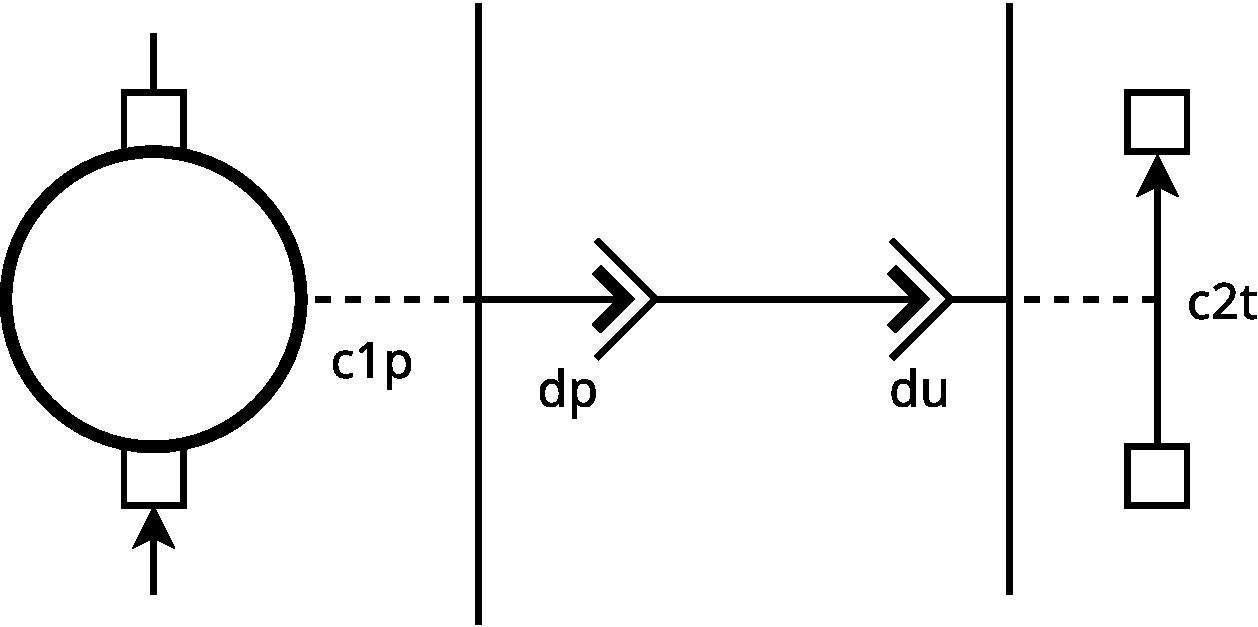
\includegraphics[scale=0.2]{images/perf_data_ports.pdf}
    \end{minipage}
  }
  \subfloat[Dependency graph]{%
    \begin{minipage}[c]{1.4\columnwidth}%
      \centering
      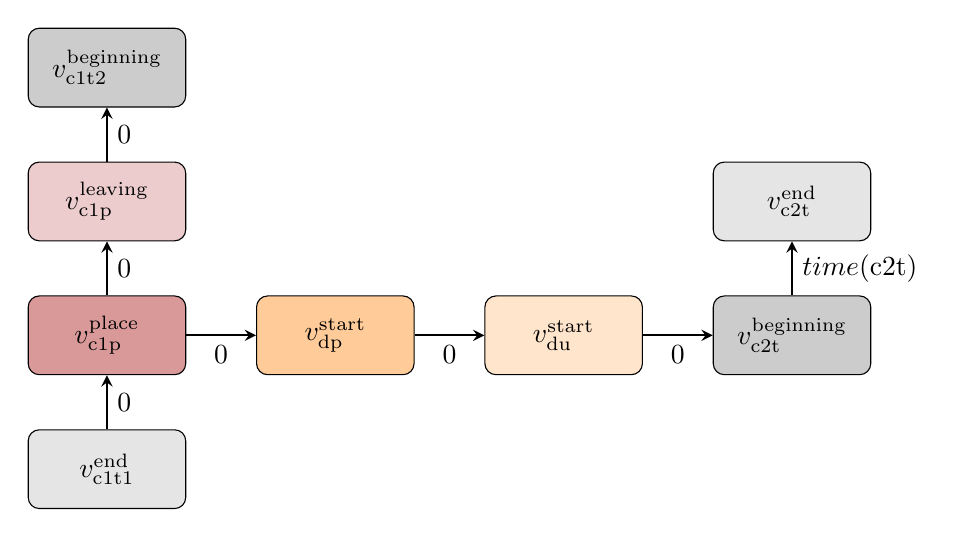
\begin{tikzpicture}[node distance=1.7cm]
        \node (c1t2) [beginning] {$v_\text{c1t2}^\text{beginning}$};
        \node (c1p1l) [leaving, below of=c1t2] {$v_\text{c1p}^\text{leaving}$};
        \node (c1p1) [place, below of=c1p1l] {$v_\text{c1p}^\text{place}$};
        \node (c1t1_end) [end, below of=c1p1] {$v_\text{c1t1}^\text{end}$};
        \draw [arrow] (c1t1_end) -- (c1p1) node[midway, right] {$0$};
        \draw [arrow] (c1p1) -- (c1p1l) node[midway, right] {$0$};
        \draw [arrow] (c1p1l) -- (c1t2) node[midway, right] {$0$};
        \node (dp) [provide_start, right of=c1p1, xshift=1.2cm] {$v_\text{dp}^\text{start}$};
        \node (du) [use_start, right of=dp, xshift=1.2cm] {$v_\text{du}^\text{start}$};
        \node (c2t) [beginning, right of=du, xshift=1.2cm] {$v_\text{c2t}^\text{beginning}$};
        \node (c2t_end) [end, above of=c2t] {$v_\text{c2t}^\text{end}$};
        \draw [arrow] (c2t) -- (c2t_end) node[midway, right] {$time(\text{c2t})$};
        \draw [arrow] (c1p1) -- (dp) node[midway, below] {$0$};
        \draw [arrow] (dp) -- (du) node[midway, below] {$0$};
        \draw [arrow] (du) -- (c2t) node[midway, below] {$0$};
      \end{tikzpicture}
    \end{minipage}
  }
  \caption{Vertices and arcs for data ports, bindings and connections}
  \label{fig:data_ports_graph}
\end{figure*}

For each connection between service provide port $p$ and service use port
$u$ in the assembly, we associate two arcs. The first from
$v_p^\text{start}$ to $v_u^\text{start}$ represents the fact that the
service may only be used after it has started being provided.
The second from $v_u^\text{stop}$ to $v_p^\text{stop}$ represents the fact
that the service may stop being provided only after it has stopped being
used.
Figure~\ref{fig:service_ports_graph} depicts the transformation of a
connection between service provide port \emph{sp} and service use port
\emph{su}.
\[
A_{L_{P}}=\bigcup_{\left(p,u\right)\in L_{P}}\left\{ \left(v_p^\text{start},v_u^\text{start},0\right),\left(v_u^\text{stop},v_p^\text{stop},0\right)\right\} 
\]

\begin{figure*}[h]
  \subfloat[Concerto assembly]{%
    \begin{minipage}[c]{0.7\columnwidth}%
      \centering
      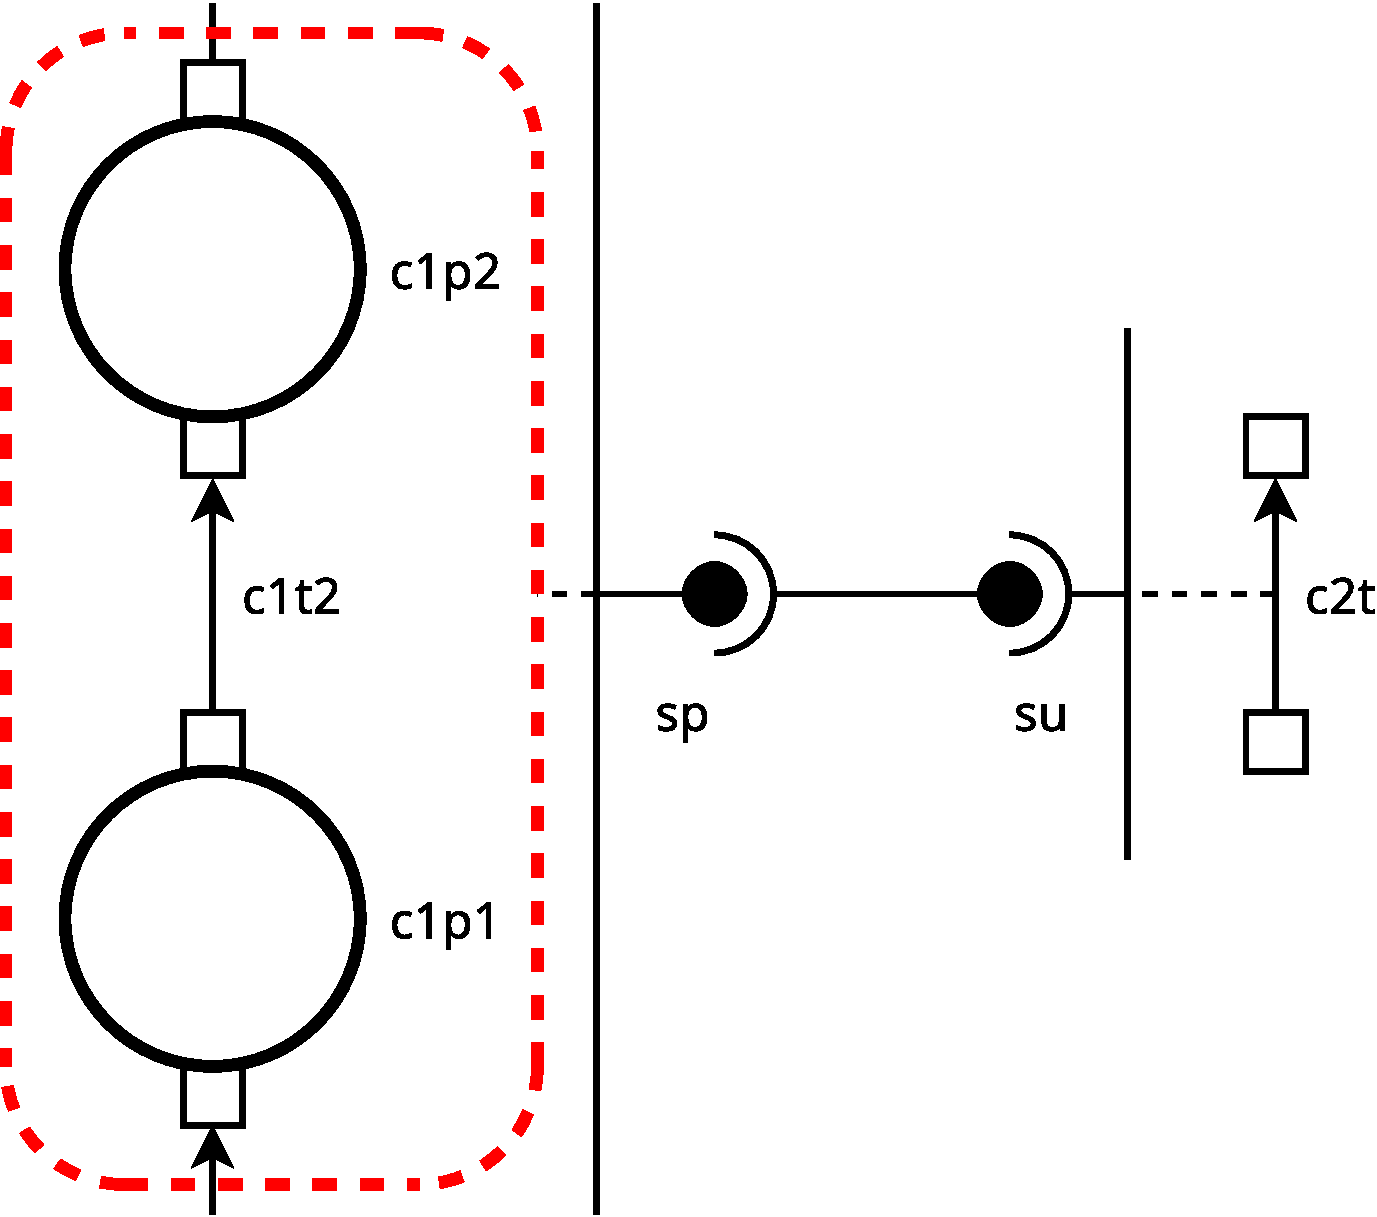
\includegraphics[scale=0.2]{images/perf_service_ports.pdf}
    \end{minipage}
  }
  \subfloat[Dependency graph]{%
    \begin{minipage}[c]{1.3\columnwidth}%
      \centering
      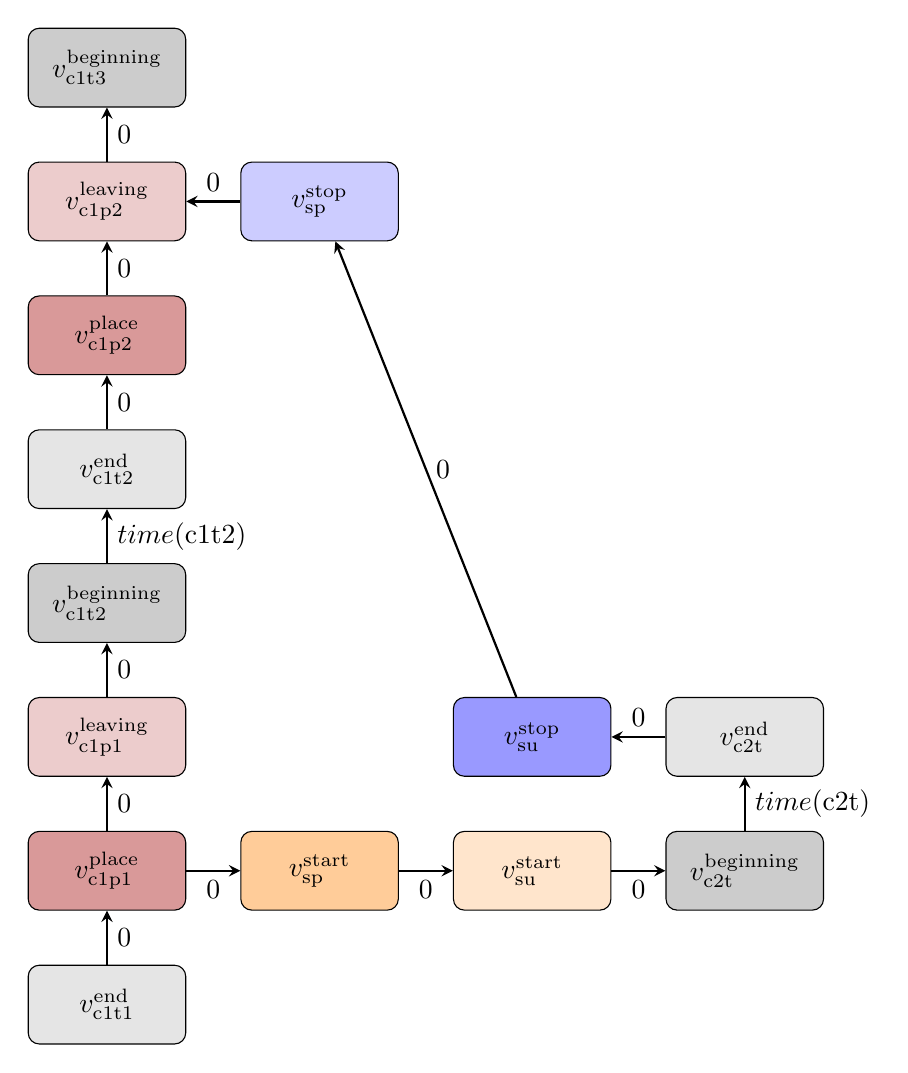
\begin{tikzpicture}[node distance=1.7cm]
        \node (c1t3) [beginning] {$v_\text{c1t3}^\text{beginning}$};
        \node (c1p2l) [leaving, below of=c1t3] {$v_\text{c1p2}^\text{leaving}$};
        \node (c1p2) [place, below of=c1p2l] {$v_\text{c1p2}^\text{place}$};
        \node (c1t2_end) [end, below of=c1p2] {$v_\text{c1t2}^\text{end}$};
        \node (c1t2) [beginning, below of=c1t2_end] {$v_\text{c1t2}^\text{beginning}$};
        \node (c1p1l) [leaving, below of=c1t2] {$v_\text{c1p1}^\text{leaving}$};
        \node (c1p1) [place, below of=c1p1l] {$v_\text{c1p1}^\text{place}$};
        \node (c1t1_end) [end, below of=c1p1] {$v_\text{c1t1}^\text{end}$};
        \draw [arrow] (c1t1_end) -- (c1p1) node[midway, right] {$0$};
        \draw [arrow] (c1p1) -- (c1p1l) node[midway, right] {$0$};
        \draw [arrow] (c1p1l) -- (c1t2) node[midway, right] {$0$};
        \draw [arrow] (c1t2) -- (c1t2_end) node[midway, right] {$time(\text{c1t2})$};
        \draw [arrow] (c1t2_end) -- (c1p2) node[midway, right] {$0$};
        \draw [arrow] (c1p2) -- (c1p2l) node[midway, right] {$0$};
        \draw [arrow] (c1p2l) -- (c1t3) node[midway, right] {$0$};
        \node (sp) [provide_start, right of=c1p1, xshift=1cm] {$v_\text{sp}^\text{start}$};
        \node (su) [use_start, right of=sp, xshift=1cm] {$v_\text{su}^\text{start}$};
        \node (c2t) [beginning, right of=su, xshift=1cm] {$v_\text{c2t}^\text{beginning}$};
        \node (c2t_end) [end, above of=c2t] {$v_\text{c2t}^\text{end}$};
        \node (sps) [provide_stop, right of=c1p2l, xshift=1cm] {$v_\text{sp}^\text{stop}$};
        \node (sus) [use_stop, left of=c2t_end, xshift=-1cm] {$v_\text{su}^\text{stop}$};
        \draw [arrow] (c2t) -- (c2t_end) node[midway, right] {$time(\text{c2t})$};
        \draw [arrow] (c1p1) -- (sp) node[midway, below] {$0$};
        \draw [arrow] (sp) -- (su) node[midway, below] {$0$};
        \draw [arrow] (su) -- (c2t) node[midway, below] {$0$};
        \draw [arrow] (c2t_end) -- (sus) node[midway, above] {$0$};
        \draw [arrow] (sus) -- (sps) node[midway, right] {$0$};
        \draw [arrow] (sps) -- (c1p2l) node[midway, above] {$0$};
      \end{tikzpicture}
    \end{minipage}
  }
  \caption{Vertices and arcs for service ports, bindings and connections}
  \label{fig:service_ports_graph}
\end{figure*}

For each initial place $\pi$ we associate one arc going from $v^\text{source}$
 to $v_\pi^\text{place}$, representing the fact that a token is placed in each
 initial place at the very beginning.
Figure~\ref{fig:source_sink_graph} depicts the transformation of two initial
places \emph{c1p1} and \emph{c2p2}.
\[
A_{I}=\bigcup_{\pi\in I_{all}}\left\{ \left(v^\text{source},v_\pi^\text{place},0\right)\right\} 
\]

In addition to the set of all initial places $I_{all}$, we define
the set of all final places $F_{all}$ as the set of places which
do not have any outgoing transition. Formally,
$F_{all}=\left\{ \pi\,\mid\,\pi\in\Pi_{all}\land\lnot\left(\exists\pi_{a}\in\Pi_{all}\,:\,\left(\pi,\pi_{a}\right)\in\Theta_{all}\right)\right\} $.
Then, for each final place $\pi$ we associate one arc going from
$v_\pi^\text{place}$ to $v^\text{sink}$, representing the fact that the
commissionning is over only after all components have reached their final places
(\ie when no more transition can be executed).
Figure~\ref{fig:source_sink_graph} depicts the transformation of three final
places \emph{c1p2}, \emph{c2p2} and \emph{c2p3}.
\[
A_{F}=\left\{ v_\pi^\text{place},v^\text{sink},0\right\} 
\]

\begin{figure*}[h]
  \subfloat[Concerto assembly]{%
    \begin{minipage}[c]{0.7\columnwidth}%
      \centering
      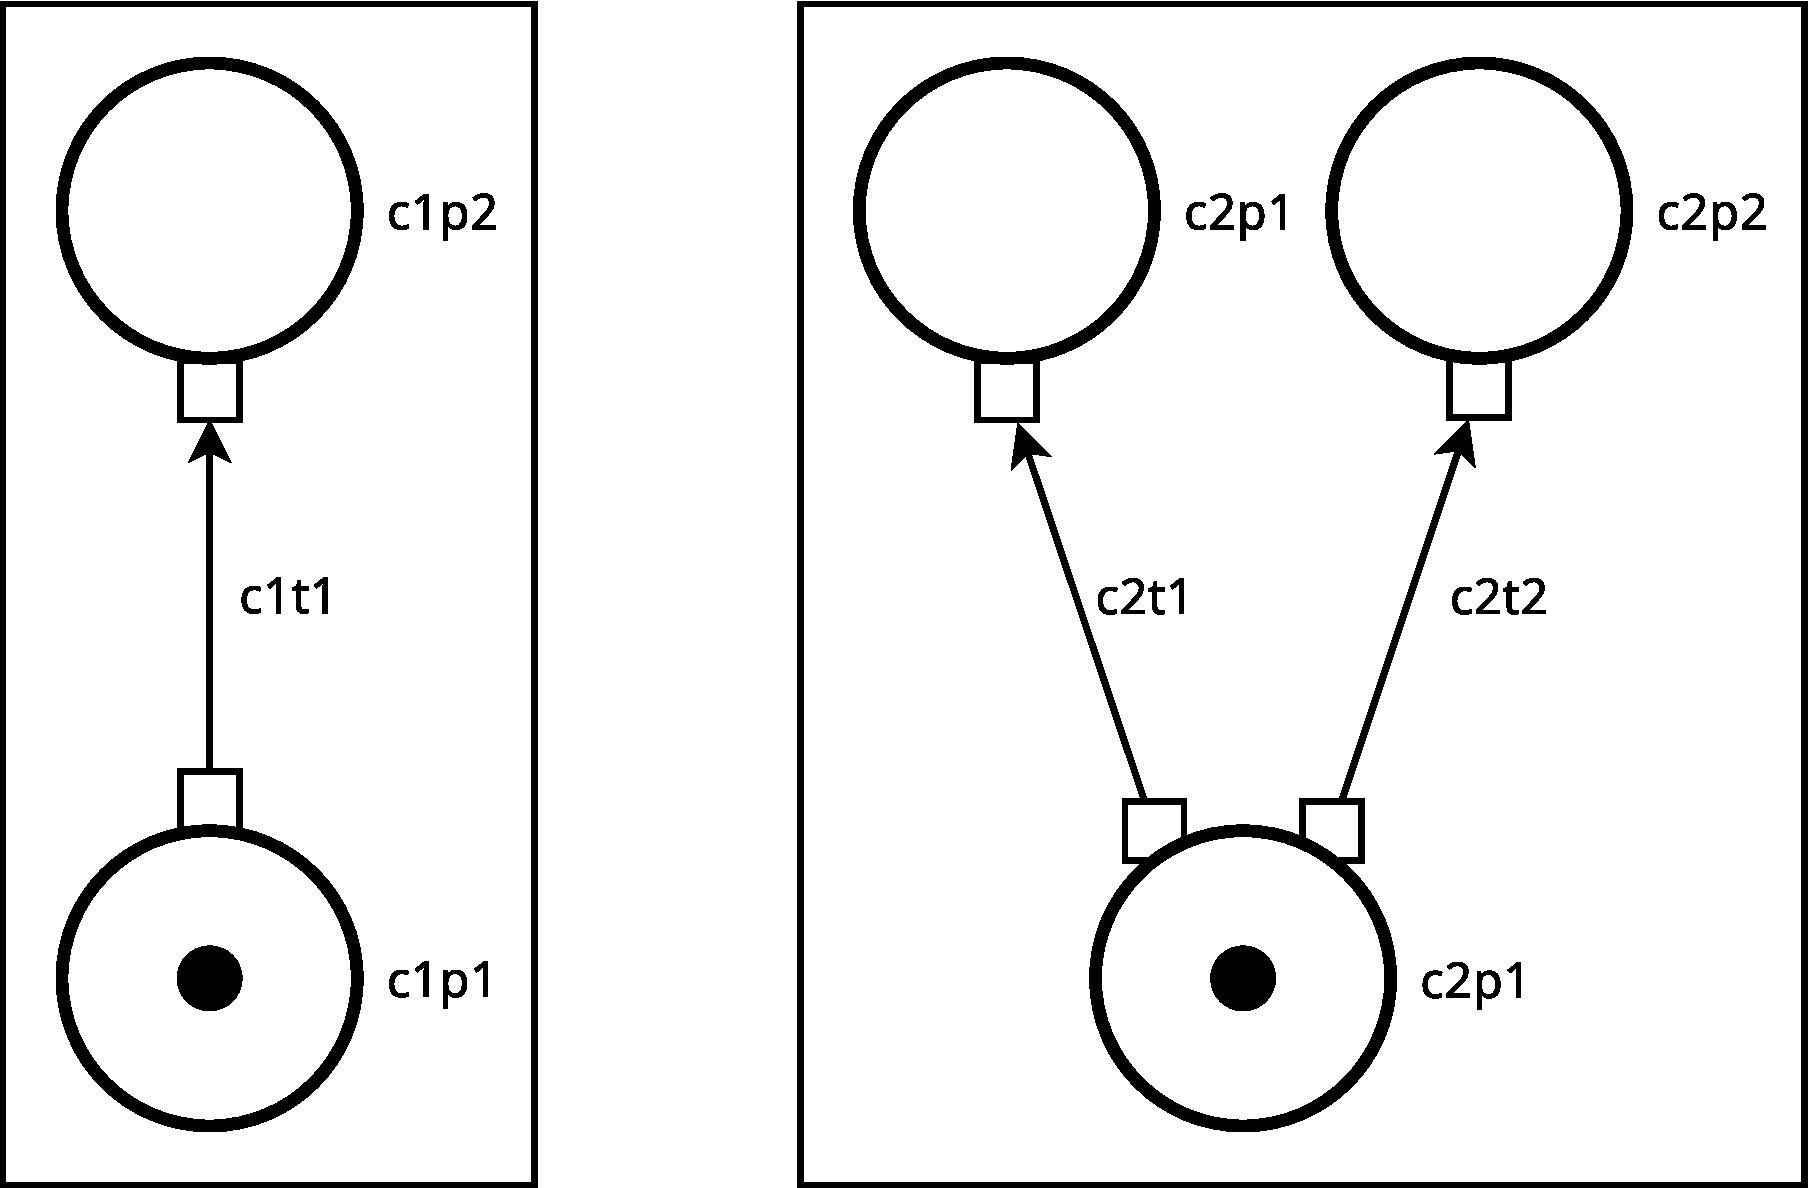
\includegraphics[scale=0.2]{images/perf_source_sink.pdf}
    \end{minipage}
  }
  \hfill
  \subfloat[Dependency graph]{%
    \begin{minipage}[c]{1.3\columnwidth}%
      \centering
      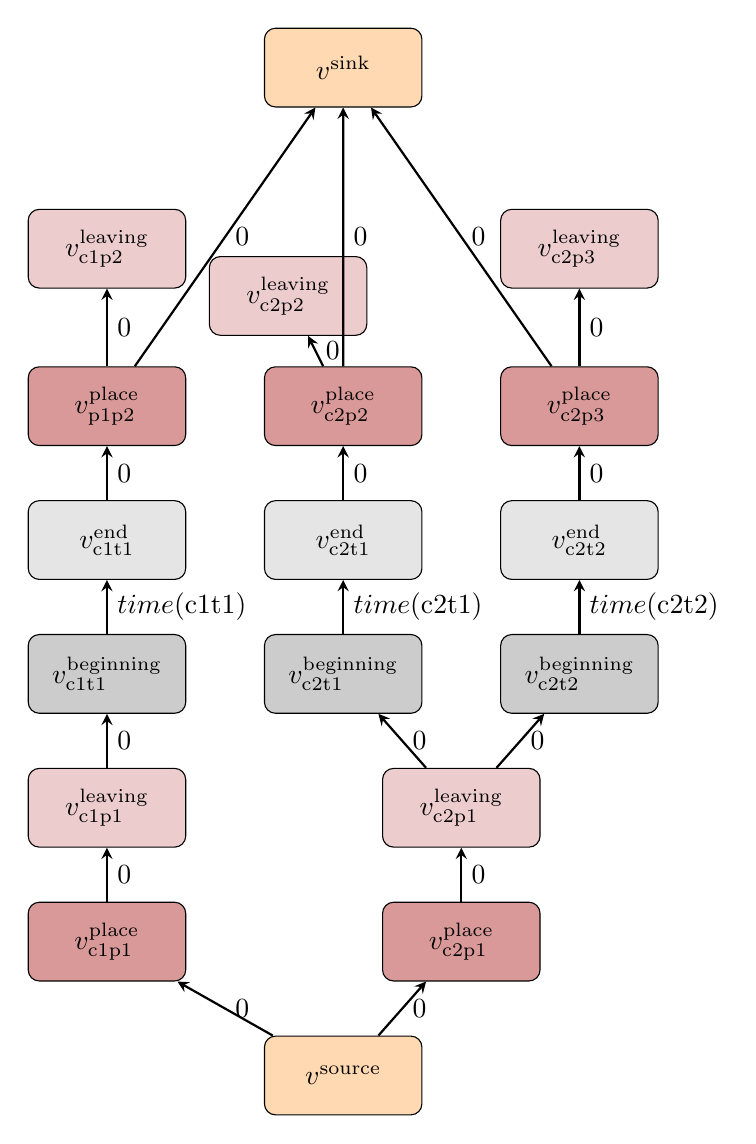
\begin{tikzpicture}[node distance=1.7cm]
        \node (c1p2l) [leaving] {$v_\text{c1p2}^\text{leaving}$};
        \node (c1p2) [place, below of=c1p2l,yshift=-0.3cm] {$v_\text{p1p2}^\text{place}$};
        \node (c1t1e) [end, below of=c1p2] {$v_\text{c1t1}^\text{end}$};
        \node (c1t1) [beginning, below of=c1t1e] {$v_\text{c1t1}^\text{beginning}$};
        \node (c1p1l) [leaving, below of=c1t1] {$v_\text{c1p1}^\text{leaving}$};
        \node (c1p1) [place, below of=c1p1l] {$v_\text{c1p1}^\text{place}$};
        
        \node (c2p2l) [leaving, right of=c1p2l, xshift=0.6cm, yshift=-0.6cm] {$v_\text{c2p2}^\text{leaving}$};
        \node (c2p2) [place, right of=c1p2, xshift=1.3cm] {$v_\text{c2p2}^\text{place}$};
        \node (c2t1e) [end, below of=c2p2] {$v_\text{c2t1}^\text{end}$};
        \node (c2t1) [beginning, below of=c2t1e] {$v_\text{c2t1}^\text{beginning}$};
        \node (c2p1l) [leaving, below of=c2t1, xshift=1.5cm] {$v_\text{c2p1}^\text{leaving}$};
        \node (c2p1) [place, below of=c2p1l] {$v_\text{c2p1}^\text{place}$};
        
        \node (c2p3) [place, right of=c2p2, xshift=1.3cm] {$v_\text{c2p3}^\text{place}$};
        \node (c2p3l) [leaving, above of=c2p3, yshift=0.3cm] {$v_\text{c2p3}^\text{leaving}$};
        \node (c2t2e) [end, below of=c2p3] {$v_\text{c2t2}^\text{end}$};
        \node (c2t2) [beginning, below of=c2t2e] {$v_\text{c2t2}^\text{beginning}$};
        
        \node (source) [control, below of=c2p1, xshift=-1.5cm] {$v^\text{source}$};
        \node (sink) [control, above of=c1p2l, xshift=3cm, yshift=0.6cm] {$v^\text{sink}$};
        
        \draw [arrow] (c1p1) -- (c1p1l) node[midway, right] {$0$};
        \draw [arrow] (c1p2) -- (c1p2l) node[midway, right] {$0$};
        \draw [arrow] (c2p1) -- (c2p1l) node[midway, right] {$0$};
        \draw [arrow] (c2p2) -- (c2p2l) node[midway, right] {$0$};
        \draw [arrow] (c2p3) -- (c2p3l) node[midway, right] {$0$};
        \draw [arrow] (c1t1) -- (c1t1e) node[midway, right] {$time(\text{c1t1})$};
        \draw [arrow] (c2t1) -- (c2t1e) node[midway, right] {$time(\text{c2t1})$};
        \draw [arrow] (c2t2) -- (c2t2e) node[midway, right] {$time(\text{c2t2})$};
        \draw [arrow] (c1p1l) -- (c1t1) node[midway, right] {$0$};
        \draw [arrow] (c2p1l) -- (c2t1) node[midway, right] {$0$};
        \draw [arrow] (c2p1l) -- (c2t2) node[midway, right] {$0$};
        \draw [arrow] (c1t1e) -- (c1p2) node[midway, right] {$0$};
        \draw [arrow] (c2t1e) -- (c2p2) node[midway, right] {$0$};
        \draw [arrow] (c2t2e) -- (c2p3) node[midway, right] {$0$};
        \draw [arrow] (source) -- (c1p1) node[midway, right] {$0$};
        \draw [arrow] (source) -- (c2p1) node[midway, right] {$0$};
        \draw [arrow] (c1p2) -- (sink) node[midway, right] {$0$};
        \draw [arrow] (c2p2) -- (sink) node[midway, right] {$0$};
        \draw [arrow] (c2p3) -- (sink) node[midway, right] {$0$};
      \end{tikzpicture}
    \end{minipage}
  }
  \caption{Arcs from source to initial places and from final places to sink. For the sake of clarity, there are no dependencies between the two components.}
  \label{fig:source_sink_graph}
\end{figure*}

Finally, we define $A$ as the union of all of these. 
\[
A=A_\Pi\cup A_{\Theta}\cup A_{D_{u}}\cup A_{D_{p}}\cup A_{P_{u}}\cup A_{P_{p}}\cup A_{L_{D}}\cup A_{L_{P}}\cup A_{I}\cup A_{F}
\]


\subsection{Time estimation}

We define the time estimation of the execution of the \mad assembly
to be the length of a longest path between $v^\text{source}$ and
$v^\text{sink}$ in $G$.

\begin{property}
If $v^\text{sink}$ is reachable from $v^\text{source}$ and $G$ has no
cycle then the time estimation is well-defined.
\end{property}

\begin{proof}
 If $v^\text{sink}$ is reachable from $v^\text{source}$, there exists at least
 one path from $v^\text{source}$ to  $v^\text{sink}$. Because there are no
 cycles, the number of paths between $v^\text{source}$ and $v^\text{sink}$ is
 finite. Because all the paths have a weight, the set of longest paths is
 well-defined (and not empty). Therefore the length of a longest path is
 well-defined.
\end{proof}

\begin{property}
  If a place \emph{pTarget} is reachable from place \emph{pStart} (distinct
  from \emph{pTarget}) in the \net of a component then $v_{pTarget}^{place}$ is reachable
  from $v_{pStart}^{place}$ in a dependency graph obtained from an assembly
  containing this component.
  \label{propertyReachable}
\end{property}

\begin{proof}
 Consider a path $P$ in the \net of the component going from \emph{pStart} to
 \emph{pTarget} (this path exists because \emph{pTarget} is reachable from
 \emph{pStart}). This path is made of a sequence of places connected by
 transitions: $P=(pStart,t1,p2,t2,\dots,t_n,pTarget)$. By construction,
 there exists a path $(v_{pStart}^{place},v_{pStart}^{leaving},v_{t1}^{beginning},v_{t1}^{end},v_{p2}^{place},\dots,\\v_{pTarget}^{place})$ in the dependency graph.
\end{proof}


\begin{property}
In a \mad dependency graph, if there is at least one component in the
assembly then $v^\text{sink}$ is always reachable from $v^\text{source}$.
\end{property}

\begin{proof}
  Let us consider one component, its initial place \emph{pi} and one of its
  final places \emph{pf}. By construction, $v_{pi}^\text{place}$ is reachable
  from $v^\text{source}$ and $v^\text{sink}$ is reachable from
  $v_{pf}^\text{place}$. The last thing to prove is that $v_{pf}^\text{place}$
  is reachable from $v_{pi}^\text{place}$.
  The end of the execution of a \mad component is defined as
  when all its tokens are in final places, \ie when there are no more
  transitions to perform. Therefore, by definition \emph{pf} is
  necessarily reachable from \emph{pi} in the \net of the component.
  We conclude by applying Property~\ref{propertyReachable}.
\end{proof}

\begin{property}
If a component is well-formed then its corresponding dependency graph has
no cycle.
\end{property}

\begin{proof}
 By construction, in the dependency graph corresponding to a component the
 vertices and arcs corresponding to places do not form cycles and are disjoint,
 so they cannot produce a cycle by themselves. Likewise, the arcs corresponding
 to port bindings have either their source vertex or their destination vertex of
 degree 1, so they cannot produce a cycle. Only the arcs corresponding to
 transitions can produce cycles. Moreover, the arcs in the dependency graph
 connect only the vertices corresponding to the places which are connected in
 the \net. This means that if there is a cycle in the dependency graph, there is
 a cycle in the \net. However, the \net of a well-formed \mad component
 has no cycle. Therefore there are no cycles in the dependency graph.
\end{proof}

\begin{property}
In an assembly with no deadlocks, if each port is bound to at most one
element (place, transition or group) and if the entry and exit sets of each group
always contain at most one place then the dependency graph corresponding to the
assembly has no cycles.
\end{property}

\begin{proof}
 If there is no deadlock in the \mad assembly, then there can be no ``crossing
 dependencies'' (see Figure~\ref{fig:deadlock}). This means that
 the activation and deactivation of two distinct sets of use and provide
 ports cannot create a cycle. This reasoning also applies to the activation
 and deactivation of a service use port and a service provide port (if they
 were to happen in a different order in the two components, the dependency
 graph would have a cycle, but because each port can be activated only once,
 there would be a deadlock in the assembly).
 \MC{À améliorer}
\end{proof}

\begin{figure}[h]
  \begin{center}
    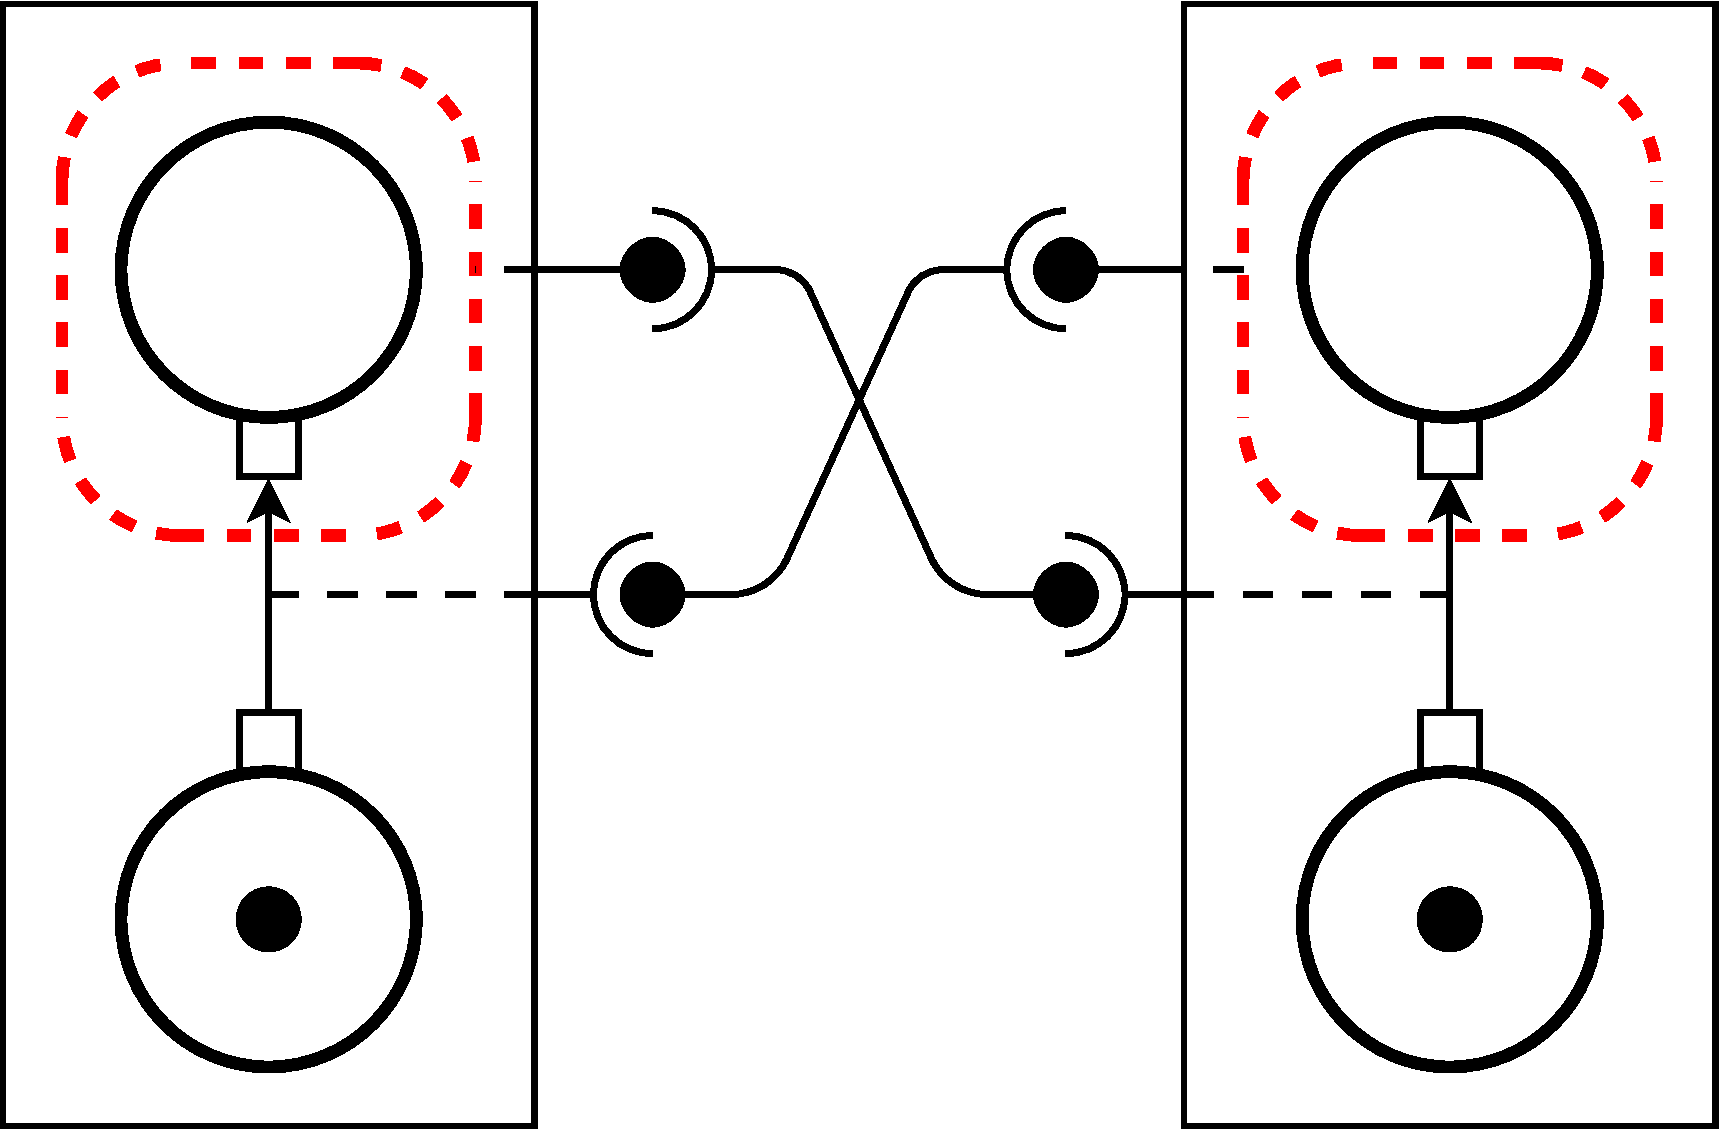
\includegraphics[width=0.7\linewidth]{./images/deadlock.pdf}
  \end{center}
  \caption{Example of an invalid assembly: crossing dependencies cause a deadlock.}
  \label{fig:deadlock}
\end{figure}

Because $G$ is a DAG, finding the longest path between $v^\text{source}$
and $v^\text{sink}$ can be done in $\mathcal{O}(|V|+|A|)$ by sorting the
vertices topologically and iterating through them, computing their maximum
distance from the source using the one of their parents. Note that
$|V| = \mathcal{O}(pl+tr+po)$ and $|A| = \mathcal{O}(tr+po+dp)$ where $pl$
is the number of places in the whole assembly, $tr$ is the number of
transitions, $po$ is the number of ports and $dp$ is the number of
dependencies. Therefore, the complexity of estimating the running time of
a \mad commissionning is $\mathcal{O}(pl+tr+po+dp)$.


\subsection{Requirements on the assembly}

In order to avoid non-determinism, which a dependency graph would not be
able to capture, we impose some requirements on a \mad assembly
for it to be compatible with the performance model. However, these
requirements are quite reasonable in the sense that none of the use
cases we have thought of do not meet these requirements.
%
First, each port may only be activated once and deactivated once, and
may only be connected to one group. Second, all groups must have a
single entry point, \ie only one transition going from a place outside
of the group to a place inside of the group. Likewise, they must have a
single exit point (if any), \ie at most one transition going from a
place inside of the group to a place outside of the group.

\subsection{Example}

\MC[Hélène]{Prendrait trop de place ? (vu la taille de la Figure~\ref{fig:source_sink_graph})}


%-------------------------------------------------------
\section{Implementation}
\label{sec:implem}
%-------------------------------------------------------
\HC[Dim]{eventually}

%-------------------------------------------------------
\section{Evaluations}
\label{sec:evaluations}
%-------------------------------------------------------
This section evaluates the performance of Madeus with empty
transitions.  Madeus is a model that relies on the description of an
\emph{internal-net} (life-cycle) for each software component of that
will be deployed. It is a low-level model, therefore the developer is
responsible for the choices of actions performed in the transitions.

The aim is to evaluate Madeus independently of any specific
transitions which is why these experiments are called
\emph{dry-runs}. It means the transitions do not contain any action
which allows to measure the overhead caused by Madeus.

% figures to add for assemblies
%Sequential

\begin{figure}[h]
  \begin{center}
    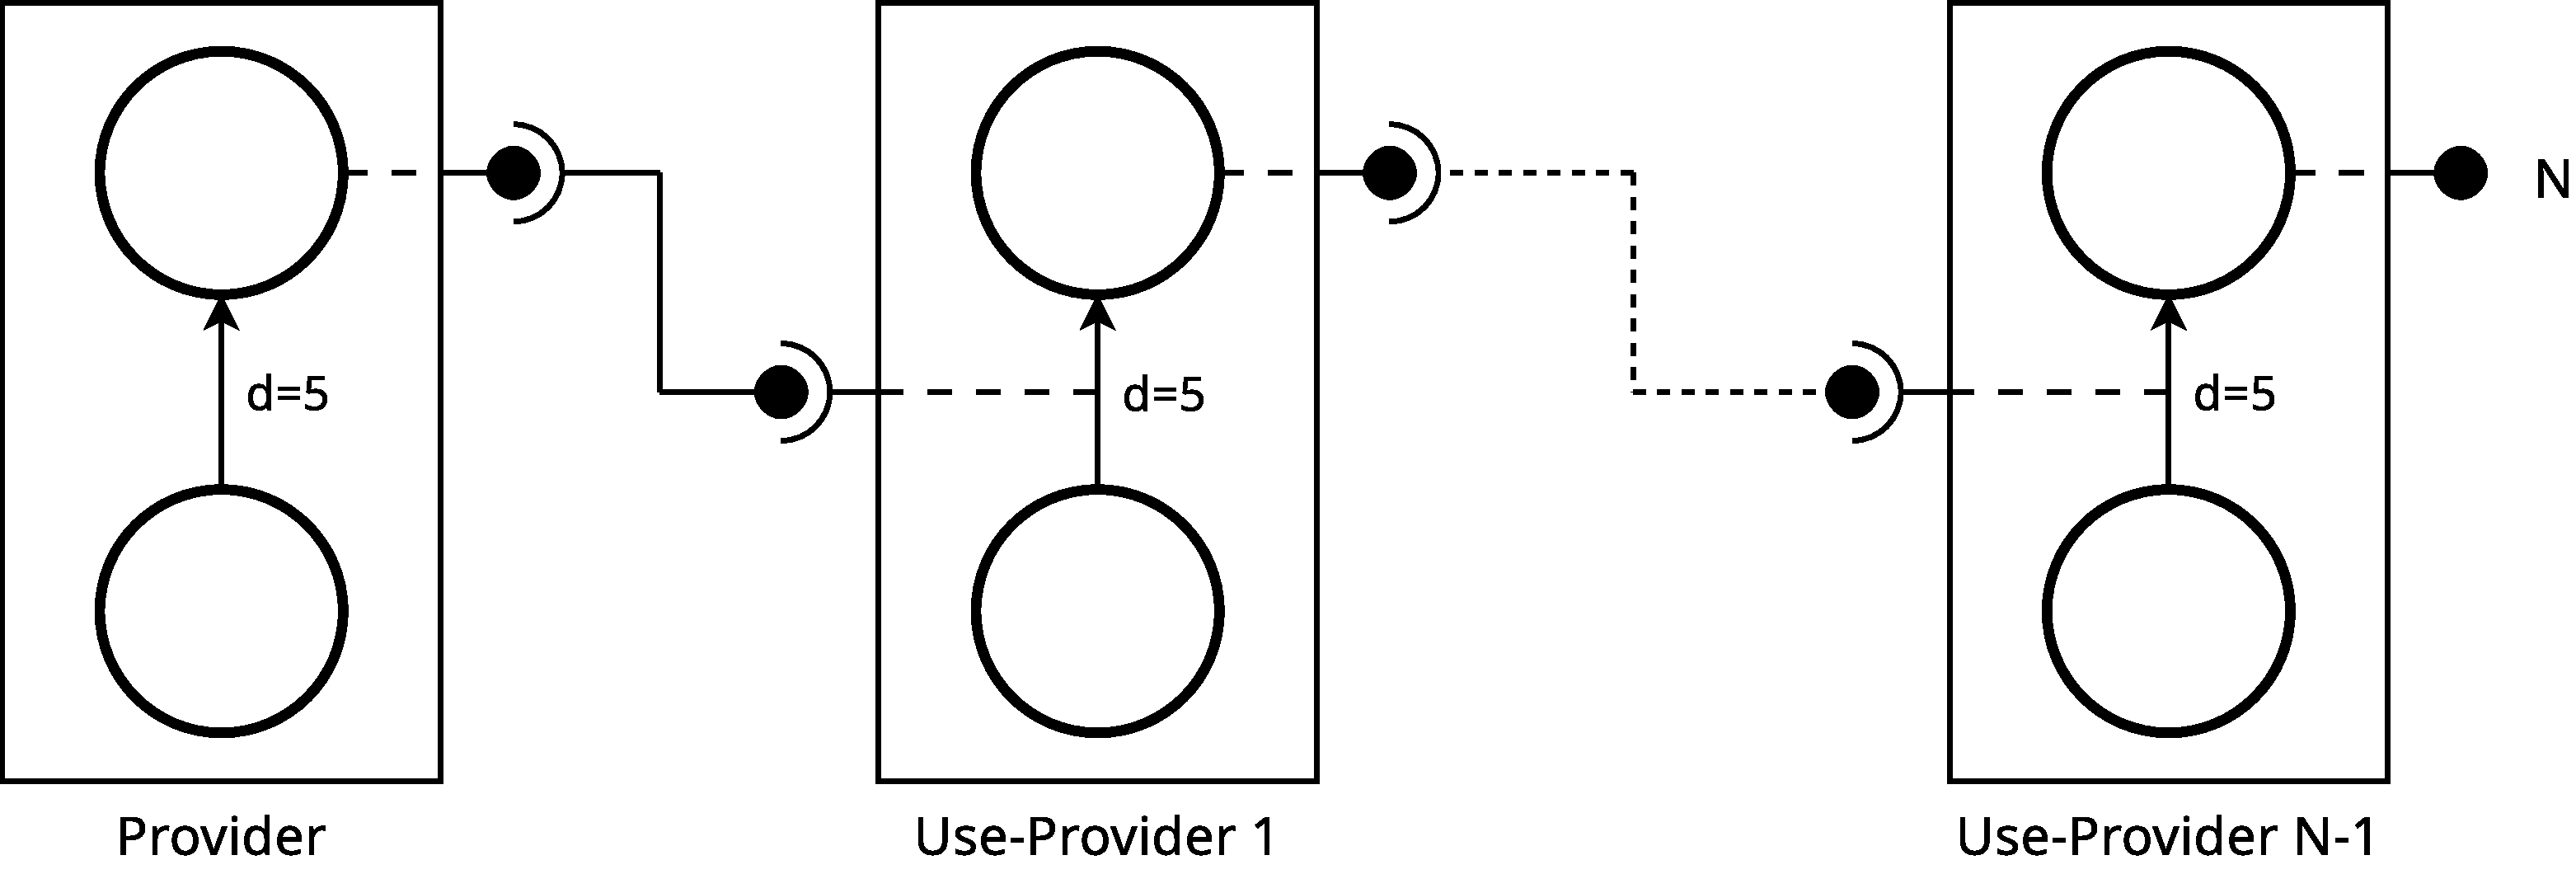
\includegraphics[width=0.4\textwidth]{./images/seq.pdf}
    \caption{The sequential assembly for the Madeus benchmark, with N components.}
    \label{fig:seq}
  \end{center}
\end{figure}

Three benchmarks compose this evaluation. The first benchmark is made
with a sequential assembly written in Madeus, depicted in
Figure~\ref{fig:seq} and made of a chain of components: one
\emph{provider} component made of a transition and two places, the
final one providing a service, and \emph{N user-provider} components
that are also composed of a transition and two places, but where the
transition uses the provide port of the preceeding component. The
components are connected and this results in a sequential execution.

A dry-run version of this assembly is built containing transitions
that do nothing besides wait for a fixed amount of time. As it is a
sequential assembly, the execution time should be increasing with the
number of \emph{N} components.

\begin{figure}[h]
  \begin{center}
    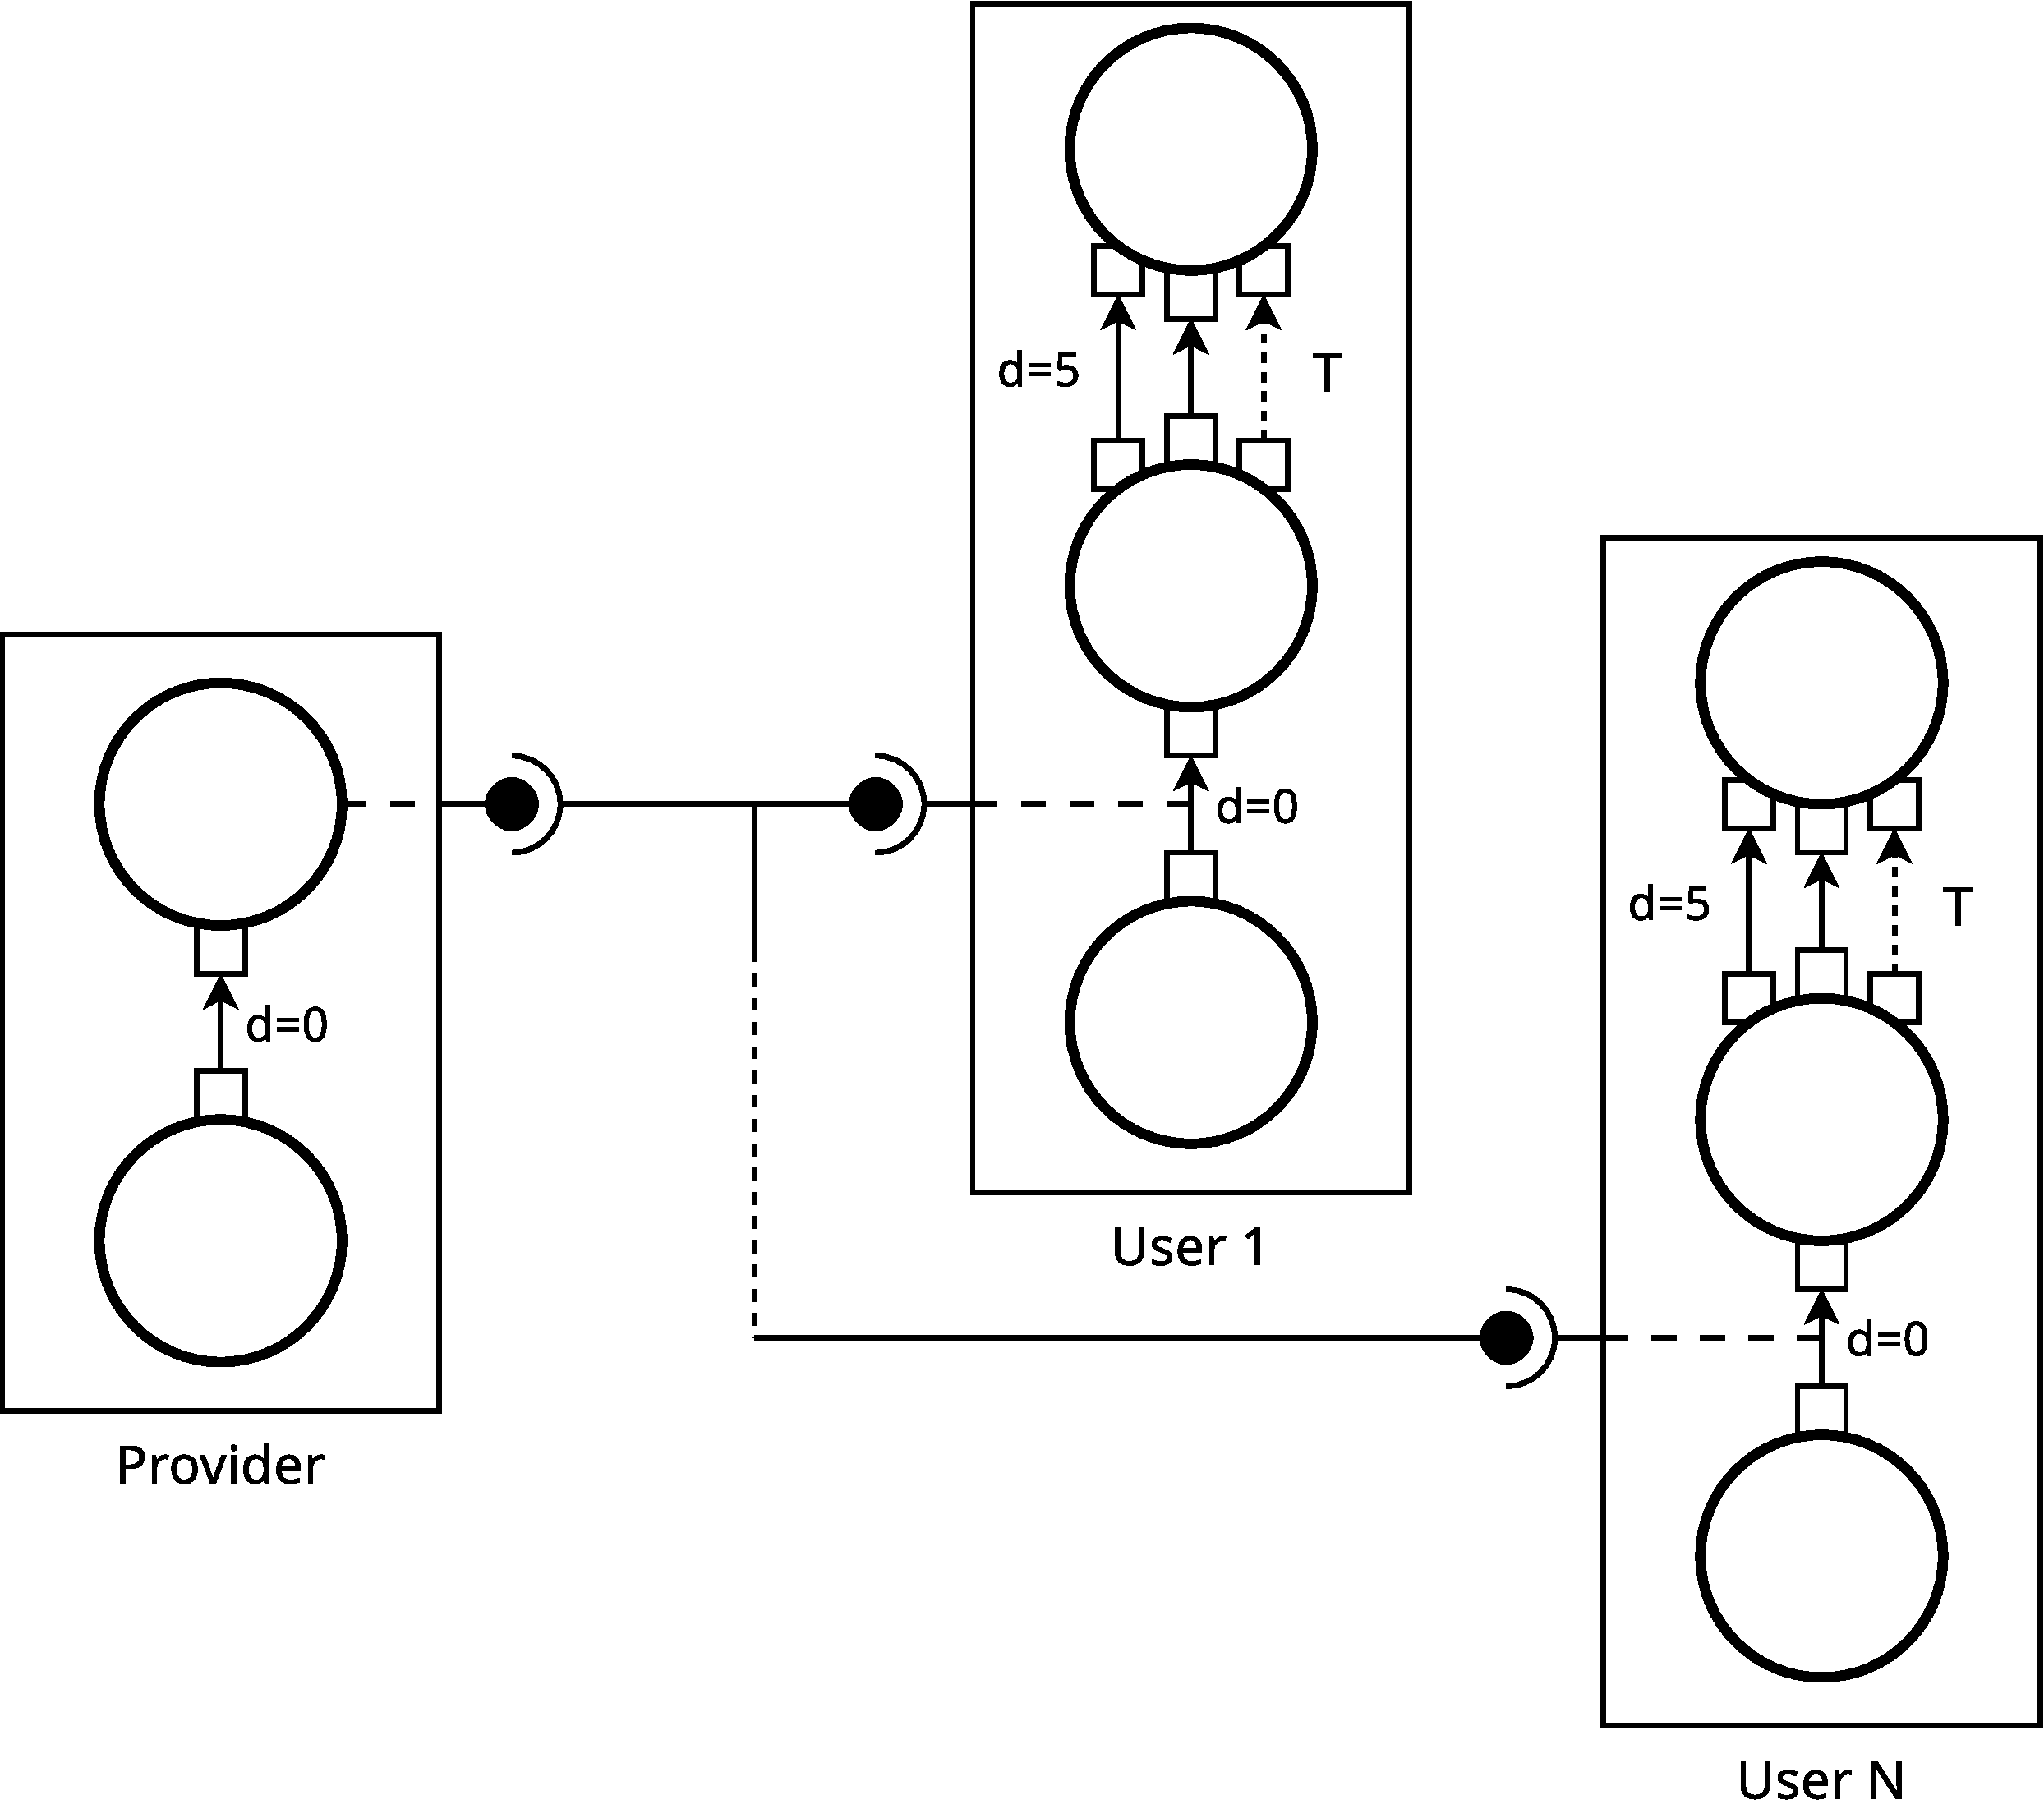
\includegraphics[width=0.4\textwidth]{./images/par.pdf}
    \caption{The parallel assembly for the Madeus benchmark, with N parallel components, and T parallel transitions.}
    \label{fig:par}
  \end{center}
\end{figure}

The second version of this assembly features a transition that calls
an ssh connection and waits for a fixed amount of time, similar as for
the dry-run version, before finishing.

Two other benchmarks made with parallel assemblies written in Madeus,
as depicted in Figure~\ref{fig:par}.  Their aim is to illustrate the
performances of Madeus regardless of the components and the content of
their transitions.

The first assembly evaluates the parallelism at the component level,
when components are deployed simultaneously and the second one
evaluates the parallelism at the transition level, when transitions
are performed simultaneously.  The second and third benchmarks are
made to evaluate the performances with parallelism both at the
component level and at the transition level.

They use the same assembly that is composed of an initial
\emph{provider} component and \emph{N parallel components} connected
to the provider. Each component contains a first transition that uses
the service provided by the provider component and \emph{T parallel
  transitions}. For the benchmark about component level parallelism,
the number of components varies from 1 to 40 components and a fixed
transition, while for the benchmark about transition level
parallelism, the number of transitions varies from 1 to
20 %link to pictures

Each benchmark was run for ten iterations with a sleep time value of 5
seconds to have a coherent scale of results. They are both evaluated
in \emph{dryrun} mode without any ssh connections and with \emph{ssh
  connections} active in the assembly between components, so as to
allow visualisation of the eventual overhead of having these ssh
connections.

\begin{figure}[h]
  \begin{center} 
    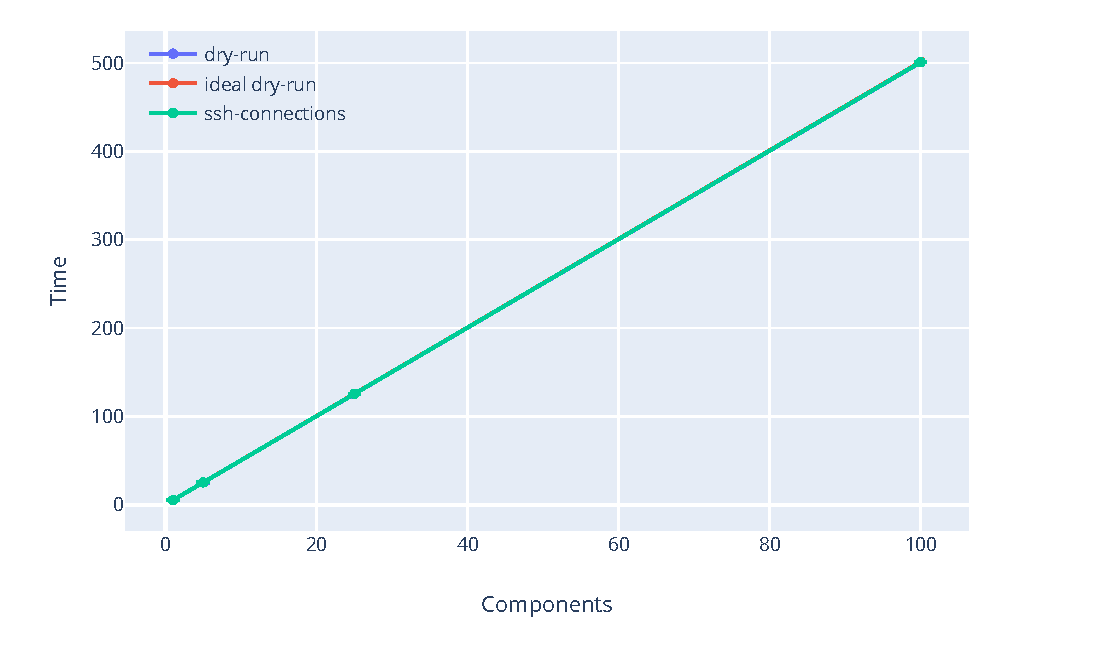
\includegraphics[width=0.5\textwidth]{./images/evaluations_sequential.pdf}
    \caption{Results of the sequential benchmark.}
    \label{fig:seqres}
  \end{center}
\end{figure}

For the sequential benchmark, we calculated the ideal curve as the sum
of all sleep times added, since they are executed sequentially from
the component assembly. The results show a linear increase in time and
the \emph{dryrun} curve follows the \emph{ideal} curve closely, as can
be seen on Figure~\ref{fig:seqres}. The difference between the
\emph{ssh-connections} curve is hard to visualise but is slightly
higher than the \emph{ideal} and \emph{dryrun} curves, a logical
result as the number of ssh connections grows with each component
added, but there is always only one ssh connection at the same time.

\begin{figure}[h]
  \begin{center} 
    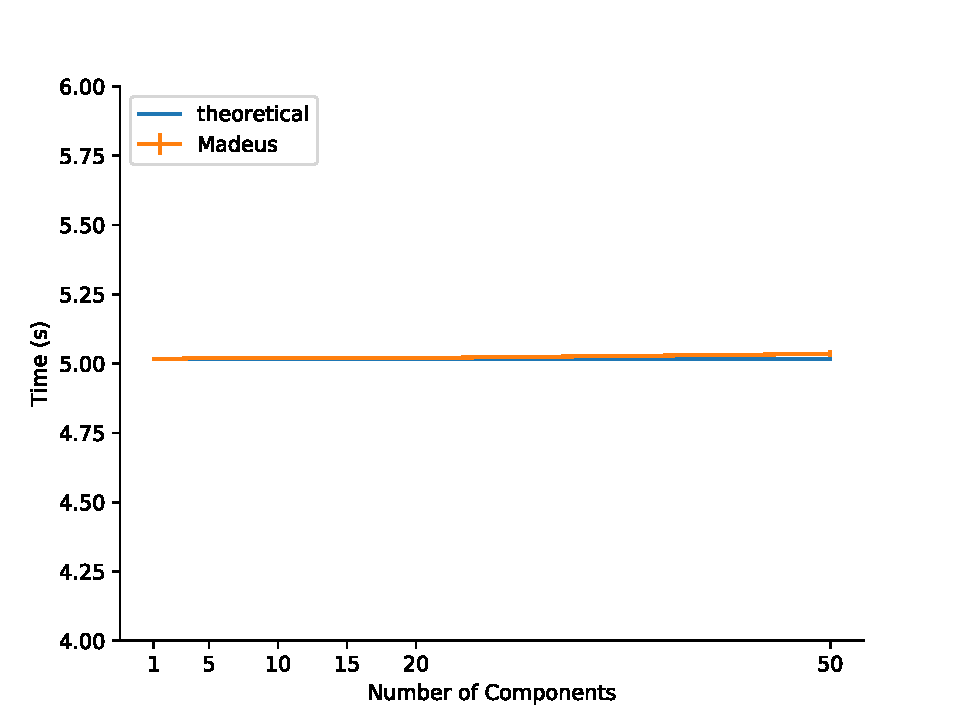
\includegraphics[width=0.5\textwidth]{./images/evaluations_par_component.pdf}
    \caption{Results of the parallel assembly benchmark with varying component number}
    \label{fig:parcompres}
  \end{center}
\end{figure}

For the results on the parallel assembly benchmark, we had to remove
one outlier data point on the parallel assembly benchmark for
component parallelism, as the first iteration of the assembly with
just one component always had 4 seconds added to the time and we could
not pinpoint the exact reason for that. As it did not occur for any of
the other iterations, we did not take it into account on the curve
drawing for our Figure~\ref{fig:parcompres}. In the results directory
that can be found on our repository we have included the original
times.json and the modified times.json files to keep the original
results intact.

The ideal curve for the parallel assembly benchmark has been
calculated with the \emph{sleep time} value on its own, if all the
components are parallelized, they all start their transition at the
same time and it should take only the \emph{sleep time} to be
finished. In \emph{dryrun} our experimental benchmark is only very
slightly above the ideal curve, which shows that Madeus does not add
significant overhead to the process when there are more
components. The \emph{ssh connection} curve allows us to see that
there is steady increase of time, adding almost 3 seconds to the
assembly deployment when reaching 40 parallel components. This show
that the overhead added by the SSH connections is not null.

\begin{figure}[h]
  \begin{center} 
    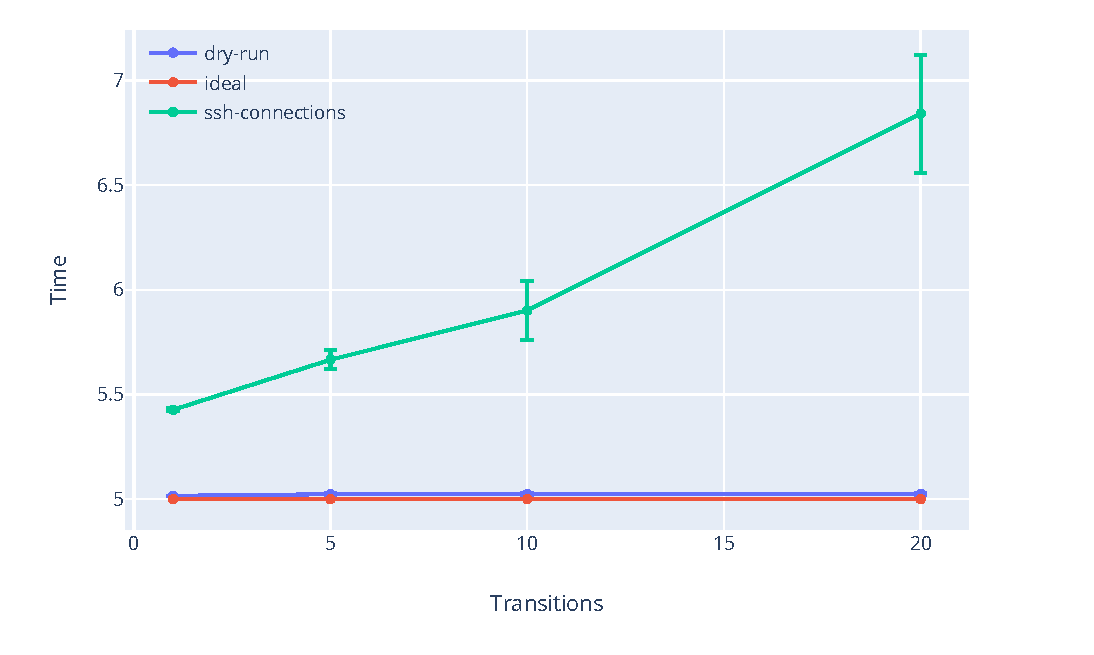
\includegraphics[width=0.5\textwidth]{./images/evaluations_par_transitions.pdf}
    \caption{Results of the parallel assembly benchmark with varying parallel transition number}
    \label{fig:partrans}
  \end{center}
\end{figure}

The results for the parallel assembly benchmark regarding parallel
transition variation are illustrated on Figure~\ref{fig:partrans}. The
calculation for the ideal curve on the parallel assembly benchmark
when varying the number of parallel transitions has been done in the
same manner as for the parallel component variation. In \emph{dryrun}
the benchmark results follow the ideal curve closely as well, whereas
the \emph{ssh connections} curve has an overhead that grows as the
number of transitions increases.

These results allow us to point out that \emph{Madeus} does not by
itself add a big overhead on the deployment. They also show the
importance of ssh connection and their impact on the deployment time.



%-------------------------------------------------------
\section{Use-cases}
\label{sec:use-cases}
%-------------------------------------------------------

\graphicspath{{images/}}

%------------------------------------
\subsection{OpenStack}
\label{subsec:openstack}
%------------------------------------

OpenStack~\cite{os:7923796} is the de-facto open-source solution to address the
IaaS level of the Cloud paradigm. Since $2010$, its community has gathered
nearly $700$ organizations (such as Google, IBM or Intel) and has produced more
than $20$ million lines of code. Its adoption is still growing in various
domains such as public administrations, e-commerce and science\footnote{See
\url{http://superuser.openstack.org/} for further information.}.

OpenStack is a large distributed software that brings together almost $100$
% TODO: Each of which en début de phrase ?
software projects. Each of which is in charge of a specific aspect of the
infrastructure management (\eg provision virtual machines, provide them with
storage, interconnect them through networks) and their cooperation is the key to
provide the features required by Cloud management.
%
Those projects are themselves composed of several software modules that are
responsible for very specific tasks (\eg placement, hypervisors, regarding
virtual machine management). While they are not all mandatory to deploy an
operable IaaS, $250$ software modules are available in those projects.
%
An OpenStack instance is a composition by the operator of those modules, which
cooperate to respond to her requirements. For instance, the operator may need
services to manage virtual rather than bare-metal machines, object storage
rather than file-systems, while VLAN networks and billing services may not be
desired in her use-case. As defined in the large OpenStack documentation, each
software module has its own commissioning process, and may depend on other
module commissioning.
%
The deployment of a typical OpenStack instance implies thus many software
modules whose commissioning process is characterized by a large amount of tasks
and interplays. As a consequence, the commissioning process of OpenStack is
complex to understand and can be very long when tasks are executed sequentially.
%
In the following, we show how the commissioning process of each OpenStack
project can be transcribed as a \mad component. Leveraging \mad enables us to
abstract tasks as transitions and express task and component coordination. As a
consequence, the \mad representation improves the global commissioning process
understandability, and can be used to reduce commissioning time by exploiting
node, intra and inter-component parallelism.
% express module interplays can help new developers to better understand both
%   code and workfow
% madeus can be used to express parallel tasks and understand module interplay

%------------------------------------
\subsection{OpenStack commissioning use-case}
%------------------------------------

\begin{table*}
  \begin{center}
    
\begin{tabular}{|c|c|c|c|c|}
   \hline
   & Roles & Places & Transitions & Ports \\
   \hline
   Nova & Manages compute instances (\eg Virtual machines) & 5 & 8 & 8\\
   Glance & Compute image store & 3 & 4 & 7\\
   Neutron & In charge of network resources & 3 & 4 & 7\\
   MariaDB & An SQL server used by most projects to store persistent
    information & 4 & 5 & 4\\
   Keystone & Manage user authentication, authorization and service
    discovery & 3 & 2 & 4\\
   RabbitMQ & The message bus for inter-service communication & 2 & 1 & 3\\
   HAProxy & Load-balances the requests to OpenStack controllers & 2 & 1 & 7\\
   OpenVSwitch & Virtualizes network functions & 3 & 1 & 2\\
   MemCached & Caches ephemeral data for most OpenStack projects & 2 & 1 & 2\\
   Facts & Collects informations about every nodes & 2 & 1 & 1\\
   Common & Common utilities (\eg cron, fluentd: a metric collector for logging)
    & 3 & 2 & 2\\
%   \hline
%   Total & 32 & 30 & 47 & \\
%   \hline
%   & Places & Transitions & Ports & Roles\\
%   \hline
%   Nova & 5 & 8 & 8 & Manage compute instances (\eg Virtual machines)\\
%   Glance & 3 & 4 & 7 & Compute image store\\
%   Neutron & 3 & 4 & 7 & In charge of network resources\\
%   Keystone & 3 & 2 & 4 & Manage user authentication, authorization and service
%    discovery\\
%   MariaDB & 4 & 5 & 4 & An SQL server used by most projects to store persistant
%    information\\
%   RabbitMQ & 2 & 1 & 3 & The message bus for inter-service communication\\
%   HAProxy & 2 & 1 & 7 & Load-balances the requests to OpenStack API services\\
%   OpenVSwitch & 3 & 1 & 2 & Virtualizes network functions\\
%   MemCached & 2 & 1 & 2 & Caches ephemeral data for most OpenStack projects\\
%   Facts & 2 & 1 & 1 & Collects inforamtions about every nodes\\
%   Common & 3 & 2 & 2 & Common utilities (\eg cron, fluentd: a
%   metric collector for logging) \\
   \hline
   Total & & 32 & 30 & 47\\
   \hline
\end{tabular}


    \caption{Number of places, transitions, ports and roles for each \mad component
        of the OpenStack assembly of Figure~\ref{fig:full}.}
    \label{tab:os}
  \end{center}
\end{table*}

\kolla is one of the most popular project for deploying OpenStack in production.
It relies on \ansible to deploy OpenStack's modules as \docker containers, and
will be considered as our reference in the rest of this section. It is highly
opinionated out-of-the-box, allowing operators to quickly deploy a basic
OpenStack instance, but enables complete customization for advanced
administrators. As a consequence, the use-case described in this section
corresponds to the default \kolla deployment, which provides the essential
mechanisms to operate an infrastructure with OpenStack.
%
To compare the performance of \kolla and \mad, we have defined $11$ \mad
components based on the \ansible roles defined in \kolla's playbooks. Their
names are built for most of them on the OpenStack project they deploy.
\Cref{tab:os} lists these components and indicates which aspect of the Cloud
management they are in charge of. Furthermore, some \mad metrics are diplayed
(\ie the number of places, transitions and ports).
%
In this table, when the number of transitions is greater or equal to the number
of places, it means that \mad can be leveraged to express parallel transitions.
Also, the more ports, the more \mad is able to coordinate interplays during the
deployment. As depicted in \cref{tab:os}, Nova, Glance, Neutron and MariaDB are
components of particular interests since they contain more transitions and ports
than the others.

\begin{figure}
  \begin{center}
    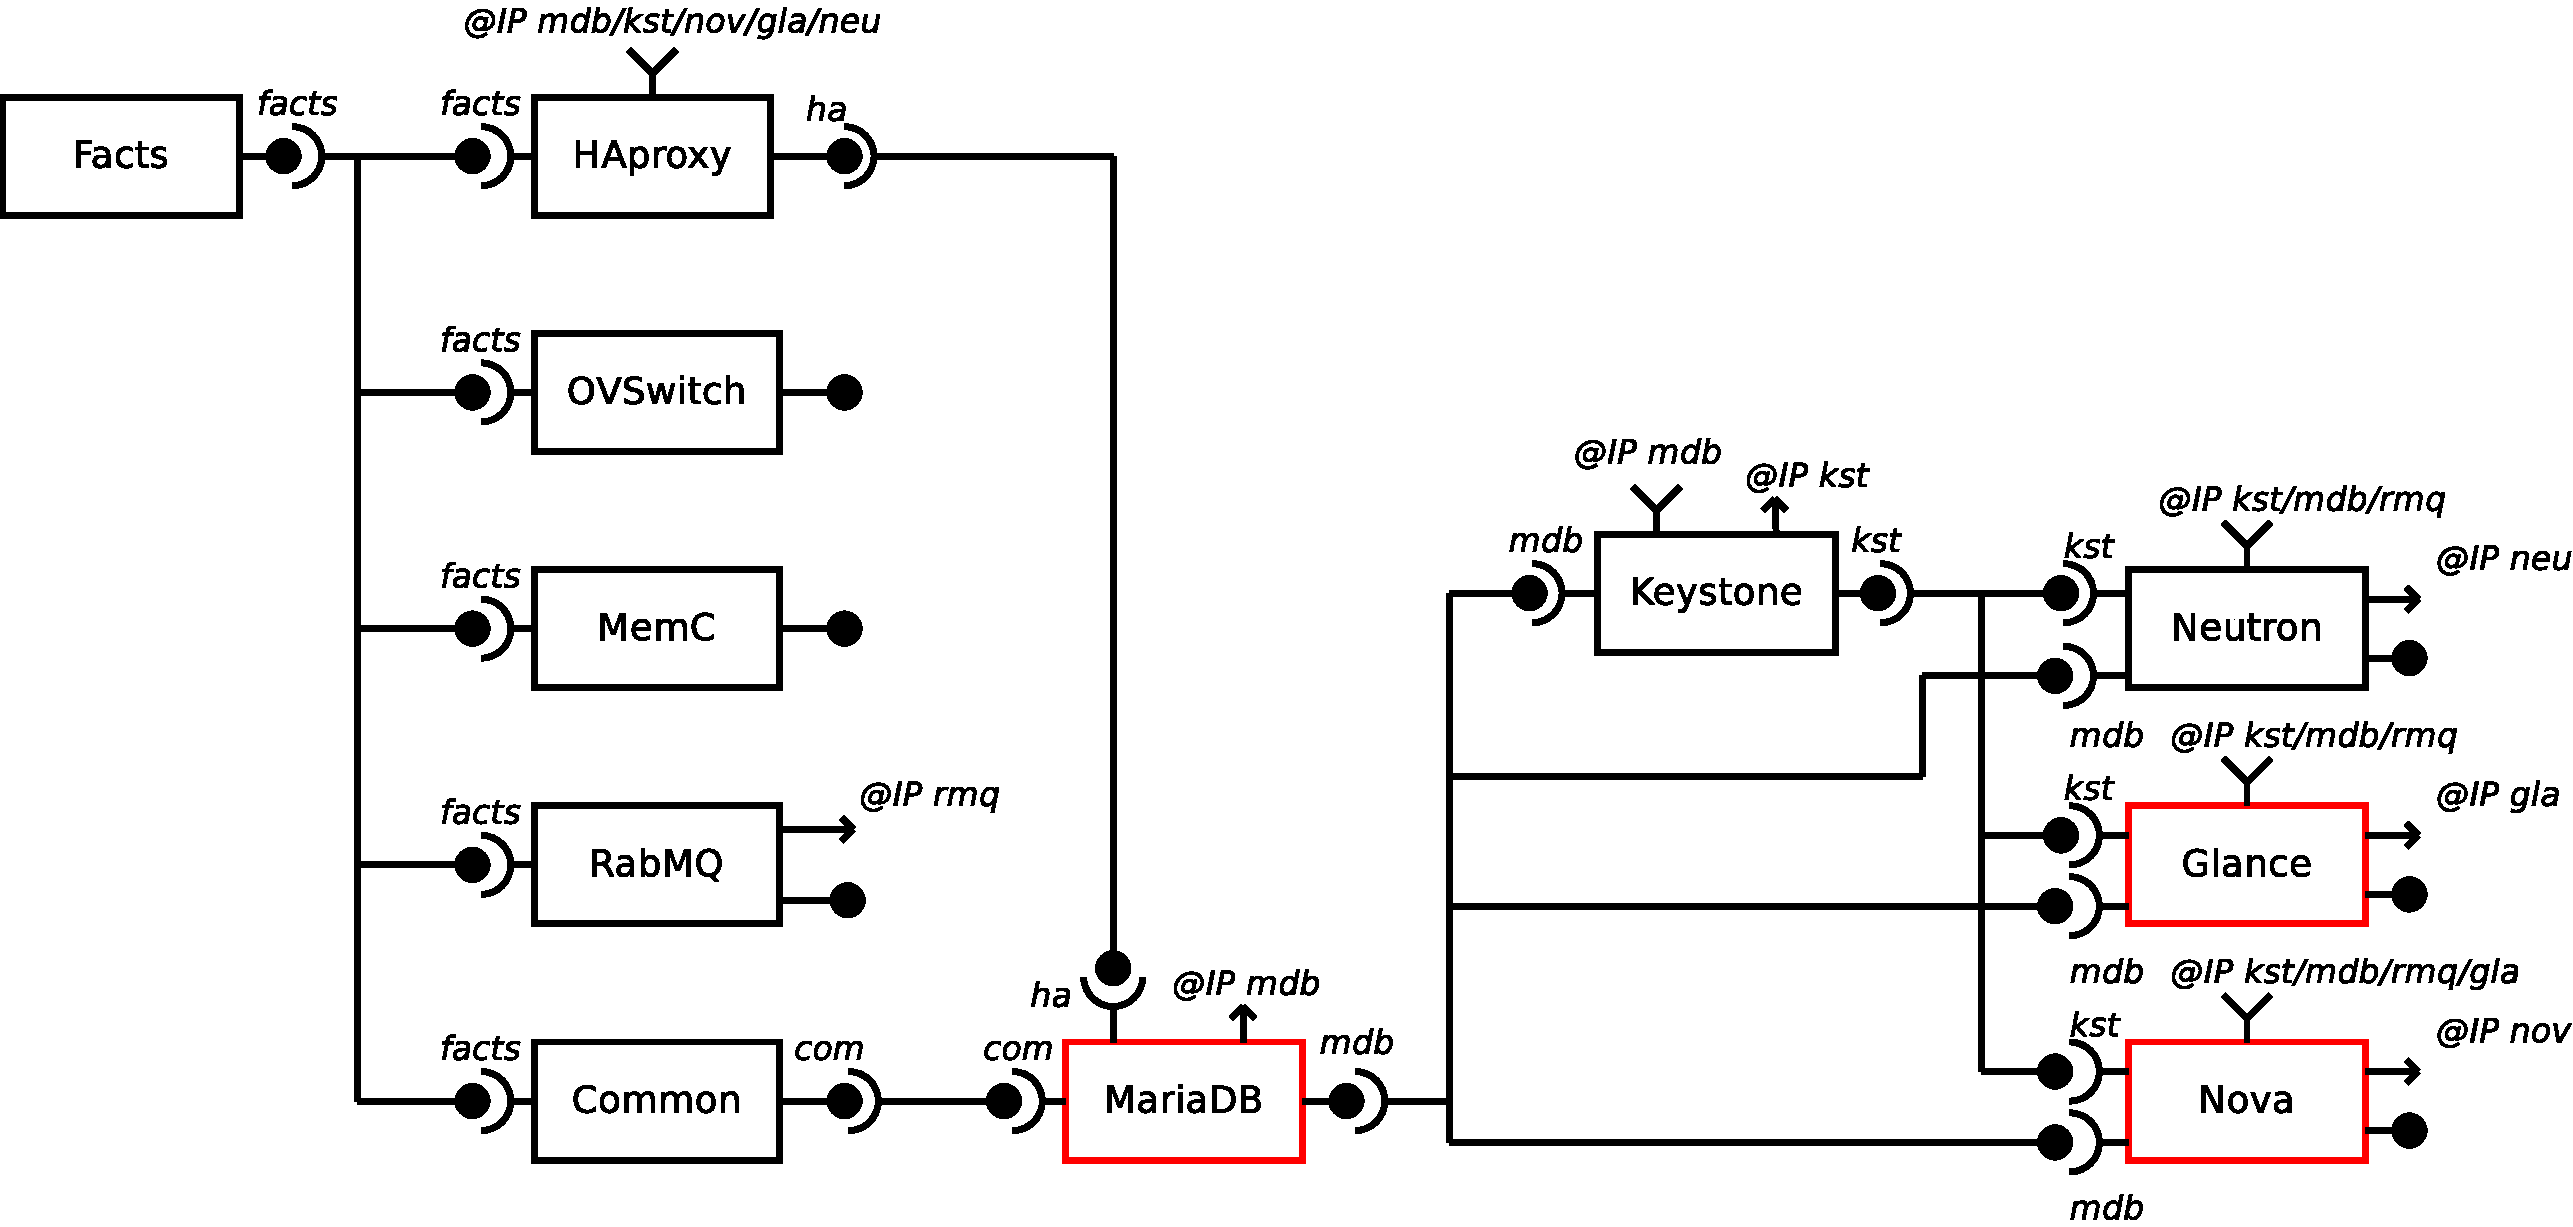
\includegraphics[width=0.5\textwidth]{./images/full.pdf}
    \caption{Simplified \mad assembly of the \kolla-based OpenStack deployment
    containing $11$ components. Connections between data ports are not depicted.
    Red components are detailed in \cref{fig:sub}.}
    \label{fig:full}
  \end{center}
\end{figure}
% TODO: Refaire cette figure en SVG pour la faire tenir sur une colonne avec
% police du papier pour que ce soit lisible

\Cref{fig:full} depicts the use-case from the operator viewpoint (\ie at the
level of the \mad assembly). For the sake of simplicity and readability, the
connections between data ports are not represented. This figure helps to
understand the high-level interplays between components. For instance, Neutron,
Glance and Nova require Keystone, while Keystone requires itself a database (\ie
MariaDB) for its commissioning process.
%MariaDB relies itself on HAProxy for being reachable through a virtual IP address.
Regarding the separation of concerns, the operator does not need to understand
component internals. She just needs to compose the desired component by listing
them and connecting them. As a consequence, a component can be replaced by
another one if they expose the same interface. For instance the operator could
replace MariaDB with MySQL: another component which also implements a database
by exposing the same ports.
% at least the same ports that are used by MariaDB

\begin{figure*}[t]
  \begin{center}
    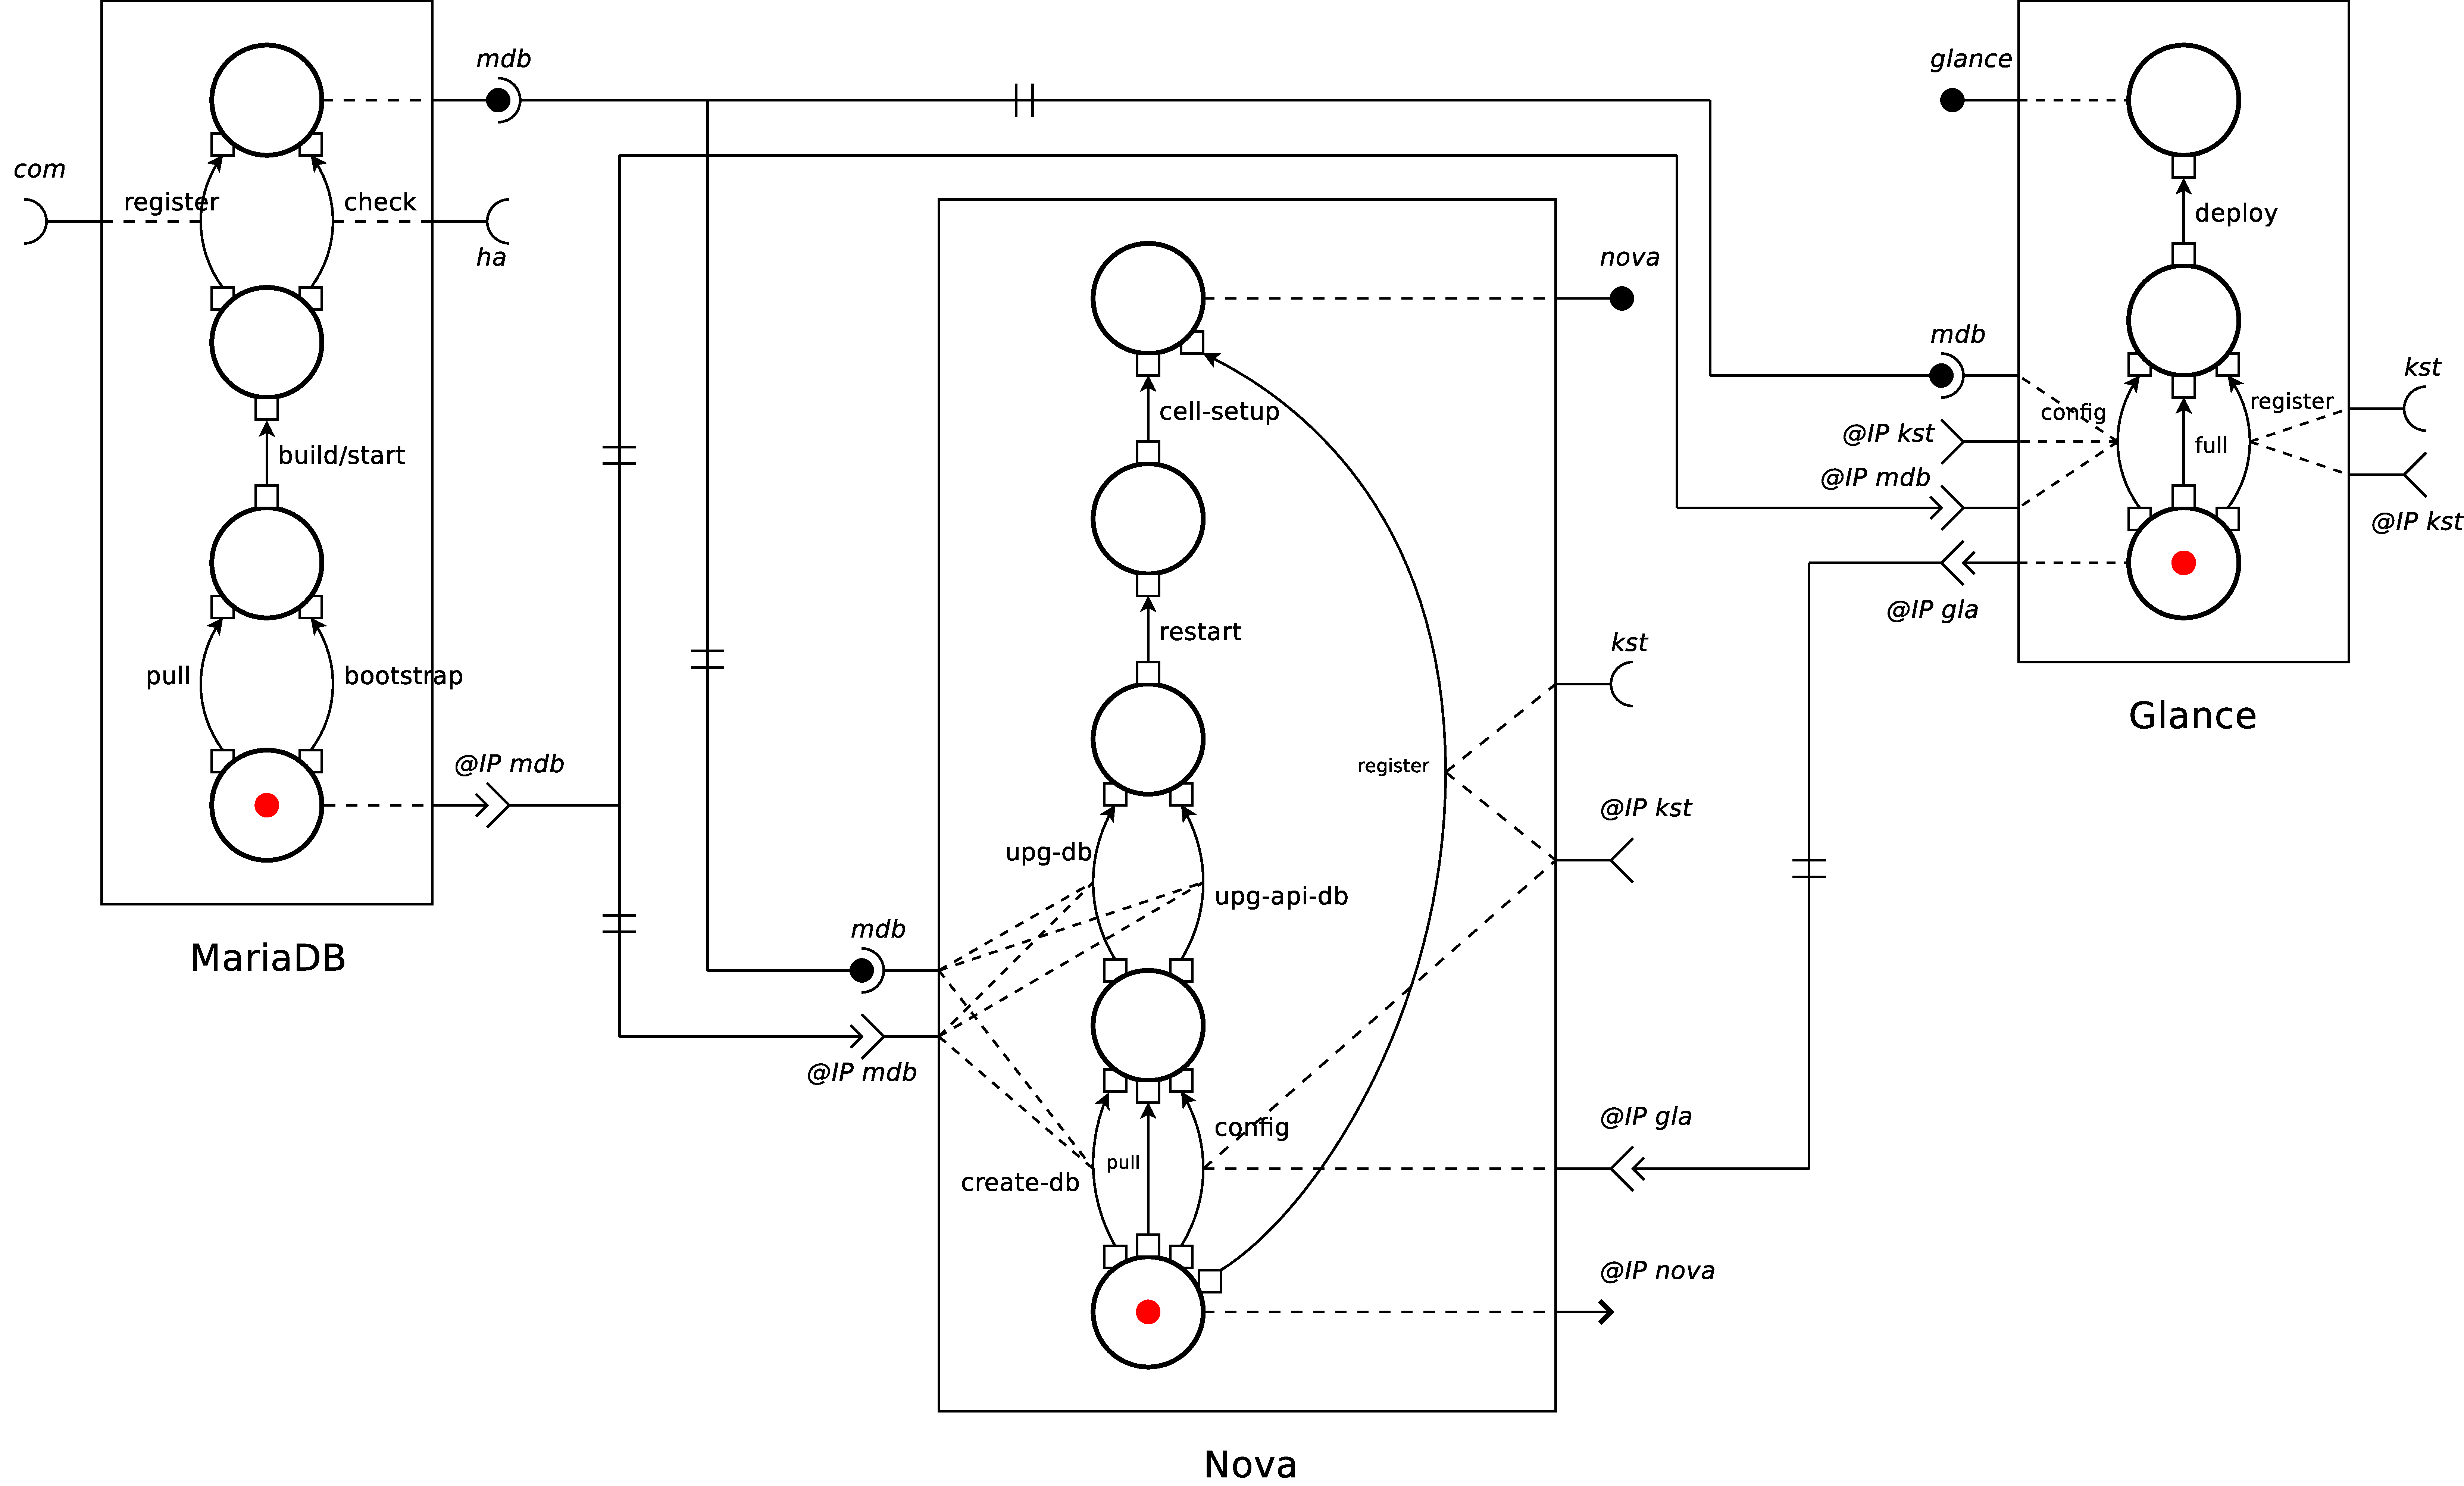
\includegraphics[width=0.8\textwidth]{./images/sub.pdf}
    \caption{A detailed sub-part of the previous component assembly to deploy
    OpenStack. The three colored components of \cref{fig:full} are detailed by
    using \mad. Black, green, blue and red tokens represent different scenarios
    during the deployment process.}
    \label{fig:sub}
  \end{center}
\end{figure*}
%TODO: Il manque les tokens de couleur dont la caption fait référence
%TODO: J'aurais peut être représenté Keystone à la place de MariaDB
%   1. Est-ce utile de dire que mariadb ici est différent de mariadb avant et
%   pas risqué pour embrouiller le message ?
%   2. Register est une transition liée à Keystone qui est très intéressante
%   quand on examine Nova (transition indépendante des autres)

We now study our use-case from the developer viewpoint, focusing on the three
colored components from \cref{fig:full}: MariaDB, Nova and Glance.
\Cref{fig:sub} depicts the internals and interplays of these components.
%
% First, the MariaDB component showed in this figure is different from the one
% depicted in \cref{fig:example}. The component here has additional content: (i)
% the transition \emph{register} that relies on the Common component; (ii) the
% transition \emph{check} that relies on HAProxy (in our use-case, MariaDB is
% reachable from HAProxy's virtual IP address). This illustrates that according to
% the type of deployment the developer or the operator aims at performing, the
% component internals may need to be modified.  Thus, it shows that being able to
% customize a component internals may be needed to improve both the expressiveness
% and efficiency of a deployment.
% TODO: récupérer de Middlware, je ne suis pas sûr que l'on garde en fonction du
% discours du papier
The dependencies previously observed at the assembly level are more
detailed at the developer level.
First, if we isolate Nova and Glance for instance, while \cref{fig:full} let us
think that Glance must be deployed before Nova, it is clear here that once Nova
obtains Glance's IP address (provided by the first place in Glance), both
components can be deployed in parallel. This shows how \mad can be leveraged for
inter-component parallelism.
%TODO: à voir si c'est pas redondant avec ce qui a été dit dans la présentation mad
Second, as we discussed before, it seemed in \cref{fig-full} that
MariaDB must be deployed before Keystone, and Keystone before
Neutron/Glance/Nova. However, with the \mad representation depicted in
\cref{fig:sub}, we understand that only the \emph{register} transition of Glance
and Nova requires the service catalog Keystone to be available (\ie to register
themselves in the catalog). We can see on the figure that other tasks can be
executed in parallel while \emph{register} waits for Keystone (\eg for Nova,
this transition is independent for all the other ones). Similarly,
\cref{fig:sub} depicts for each component many parallel transitions showing how
\mad can be leveraged for intra-component parallelism in this use-case.

%------------------------------------
\subsection{Experimental Setup and Parameters}
% ------------------------------------

% Ici on décrit nos paramètres et le testbed
This section defines first the experimental setup: (i) how modules are
distributed among nodes and (ii) the testbed characteristics. Then we describe
the different parameters used during our experimentation: (iii) the assemblies
we designed to compare our contribution with the related work and (iv) the way
\docker images are fetched by nodes.

\paragraph{Node roles and module distribution}
Each of the $11$ components defined earlier in \kolla is in charge of a
OpenStack project. As we said previously, each OpenStack project contains
multiples software modules. Hence, each component actually deploys different
modules ($36$ in total). A basic multi-node \kolla deployment targets three
nodes. First, the \emph{Control} node which hosts control services, APIs and
databases, commissions $16$ services. The second one is the \emph{Network} node
that hosts network agents and HAProxy, and contains $11$ services. Finally, the
\emph{Compute} node, in charge of compute services and where guest VMs live,
hosts $9$ services.

\begin{table}
  \begin{center}
    \small
    
\begin{tabular}{|c|c|c|c|}
   \hline
   Cluster & CPU & Memory & Network\\
   \hline
   Nova & 2 x Intel Xeon E5-2620 v4 & 64GB & 10Gbps\\
   (lyon) & 8 cores/CPU &  & \\
   \hline
   Taurus & 2 x Intel Xeon E5-2630 & 32GB & 10Gbps\\
   (lyon) & 6 cores/CPU & & \\
   \hline
   Sol & 2 x AMD Opteron 2218 & 4GB & 1Gbps\\
   (sophia) & 2 cores/CPU & &\\
   \hline
\end{tabular}


    \caption{Grid'5000 cluster configurations.}
    \label{tab:g5k}
  \end{center}
\end{table}

\paragraph{Testbed and resource provisioning}
Our evaluations have been conducted on two clusters from the experimental
platform Grid'5000\footnote{\url{www.grid5000.fr}}: \ecotype and \nova. \Cref
shows the hardware configuration for both clusters. The cluster \ecotype has a
better hardware configuration than the latter, regarding CPU, memory and network
interfaces, as detailed in the table. To design reproducible benchmarks, we
used EnosLib\footnote{\url{https://gitlab.inria.fr/discovery/enoslib}}, a
library to build experimental frameworks on multiple testbeds (\eg Grid5000,
LibVirt), and
Execo\footnote{\url{http://execo.gforge.inria.fr/doc/latest-stable/index.html}},
another library for prototyping experiments. Since \kolla, our reference, does
not manage resource provisioning, we do not include this phase in the use-case,
nor in our benchmark. Even if resource provisioning could be managed by \mad,
this step is left to EnosLib.
% TODO à voir si ça n'a pas été présenté par Maverick avant

\paragraph{Assemblies}
Our performance evaluation compares three different assemblies that are designed
to capture the behavior of \ansible, \aeolus and \mad. To that end, the
component internals for each assembly vary with regards to the number of
places, transitions and ports. It is also important to understand that we re-use
the \ansible files already provided by \kolla by splitting them into component
transitions. By using \mad to coordinate \ansible execution, it is possible for
us to provide a way to fairly compare these solutions.
The first assembly, called \ansass matches the \kolla-ansible
commissioning process. Each component is triggered sequentially, in the same way
and order as \ansible triggers sequentially the roles defined in \kolla. Since
there is no coordination between components, their internals are composed of two
states connected by a single transition which performs all the commissioning
tasks, such as in \kolla (\ie no intra-component parallelism). Each time a
component is deployed, it activates the commissioning process of the next one
(\ie no inter-component parallelism). This assembly features the first level of
parallelism which is managed by \ansible when tasks are mapped to multiple
nodes.
%The assembly is similar to the one presented in Figure\ref{fig:benchA}.
%
The second assembly, called \aeoass is equivalent to an \aeolus
commissioning of OpenStack. It provides parallelism at the component level, and
no parallelism at the task level. Coordination is driven by component's ports.
In this assembly, most components are built with two sequential transitions.
When the assembly is initiated, the first transition of those components are
triggered, while the second one is conditioned by a dependency from another
component.
%
The third assembly, called \madass, leverages our contribution to
commission OpenStack. It corresponds to the one we previously described when
presenting the use-case. All the components have their own internals definition,
based on our understanding of the OpenStack commissioning process. As depicted
previously in \cref{tab:os}, most components are built on multiple states and
transitions. This assembly relies on \mad to handle inter and intra-component
parallelism.

\begin{table}
  \begin{center}
    
\begin{tabular}{|c|c|c|c|}
   \hline
   & Compute & Network & Control\\
   \hline
   Number of images & $9$ & $11$ & $16$\\
   \hline
   Total Size (MB) & $2767$ & $2705$ & $4916$\\
   \hline
\end{tabular}


    \caption{Number of \docker images per node and their cumulated size in MB to
      download from the registry.}
    \label{tab:images}
  \end{center}
\end{table}

\paragraph{Docker container registry}
Finally, since \kolla relies on \docker containers, fetching \docker images has a
significant impact on our results: images have to be downloaded, before being
decompressed. To be as neutral as possible we have conducted experiments with
three different modes for handling those images: (1) \emph{cached}, in this mode,
images are previously placed on OpenStack nodes, so fetching \docker images has
no impact on our results; (2) \emph{local} where images are previously
downloaded on a new dedicated node of the cluster, from which images can be
loaded (\ie a local \docker registry); (3) \emph{remote} in which images are
fetched from an Internet repository (\ie the DockerHub registry).
\Cref{tab:images} gives for each OpenStack node (\ie Compute, Network and
Control) the number of \docker images to download and their compressed size.
As depicted in this table, more than $10$GB must be downloaded in our use-case.
Furthermore, the control node has to download almost twice as much data than the
other nodes.

%------------------------------------
\subsection{Results}
%------------------------------------

In this section, we analyze the results of our benchmark through different
aspects: (i) the impact of assemblies; (ii) the precision of the performance
model; (iii) the influence of registry modes and (iv) how clusters affect our
results.

\begin{figure}[t!]
  \begin{center}
    \def\svgwidth{\columnwidth}
    \subfloat[Performance comparison on \ecotype]{
      \input{./images/use_case_ecotype_perf.pdf_tex}
      \label{fig:ecotype}
    }
    \def\svgwidth{\columnwidth}
    \subfloat[Performance comparison on \nova]{
      \input{./images/use_case_nova_perf.pdf_tex}
      \label{fig:nova}
    }
    \caption{Recorded time in seconds for OpenStack commissioning with different
    clusters, assemblies and registry modes. Upper parts represent mean values
    with relative ratios for each result compared to our reference \ansass.
    Lower parts display means, standard deviations and the minimum and maximum
    values computed from the performance model, depicted as boxes.}
    \label{fig:openstack_results}
  \end{center}
\end{figure}

\begin{table}
    \begin{center}
        
\begin{tabular}{cll|ccc}
\toprule
& & & remote & local & cached  \\

\midrule
\multirow{9}{*}{\STAB{\rotatebox[origin=c]{90}{measured}}} & \multirow{3}{*}{\STAB{\rotatebox[origin=c]{90}{mean}}}  & ansible  &
530s  &
480s  &
331s  \\
  & & aeolus  &
263s  &
256s  &
229s  \\
  & & madeus  &
152s  &
148s  &
128s  \\
\cmidrule{2-6}& \multirow{3}{*}{\STAB{\rotatebox[origin=c]{90}{gain}}}  & ansible  &
0\%  &
0\%  &
0\%  \\
  & & aeolus  &
50\%  &
46\%  &
30\%  \\
  & & madeus  &
71\%  &
69\%  &
61\%  \\
\cmidrule{2-6}& \multirow{3}{*}{\STAB{\rotatebox[origin=c]{90}{std}}}  & ansible  &
1s  &
1s  &
0s  \\
  & & aeolus  &
2s  &
1s  &
1s  \\
  & & madeus  &
4s  &
4s  &
3s  \\
\midrule
\multirow{6}{*}{\STAB{\rotatebox[origin=c]{90}{theoretical}}} & \multirow{3}{*}{\STAB{\rotatebox[origin=c]{90}{max}}}  & ansible  &
540s  &
485s  &
334s  \\
  & & aeolus  &
269s  &
259s  &
232s  \\
  & & madeus  &
156s  &
158s  &
136s  \\
\cmidrule{2-6}& \multirow{3}{*}{\STAB{\rotatebox[origin=c]{90}{min}}}  & ansible  &
523s  &
473s  &
326s  \\
  & & aeolus  &
257s  &
249s  &
223s  \\
  & & madeus  &
141s  &
143s  &
123s  \\
\bottomrule
\end{tabular}

        \caption{Measured and theoretical results of our benchmark.}
        \label{tab:openstack_results}
    \end{center}
\end{table}

In these different studies, we will refer to \cref{fig:ecotype,fig:nova} which
respectively show our results on \ecotype and \nova clusters. The upper part
displays the recorded times to commission OpenStack as a function of the three
different studied assemblies.
For a better understanding of the comparison, the value of each result is
written on top of bars, while the ratio compared to \ansass, our reference, is
displayed at the bottom of bar edges.
Furthermore, for each assembly on the X-axis, the results for the three \docker
registry settings are displayed with different colors (\ie blue, red and green
for \emph{remote}, \emph{local} and \emph{cached} respectively).
On the lower part, the means for each result are depicted as horizontal lines,
the related standard deviations are represented by vertical lines, while boxes
represent the minimum and maximum values computed with the performance model.
For the sake of readability, the scale of the lower parts are different. Each
result corresponds to the average computed from $10$ iterations. The
corresponding numerical values are also displayed in
\cref{tab:openstack_results}.
% Et bien ça en fait un beau paragraphe pour seulement expliquer comment
% fonctionne la figure ^^'...

\paragraph{Impact of assemblies}

We now compare the time measured to commission OpenStack regarding the three
assemblies defined previously: \ansass, \aeoass and \madass (the lower, the
better in \cref{fig:ecotype}).
% TODO check if 10 iteration is true for all the submitted results... :)
As expected, the time required to commission these assemblies reflects the level
of parallelism they handle. Since \ansass is limited to the first
parallelism level, its commissioning time is longer than \aeoass. By
featuring inter-component parallelism, the latter outperforms the former from
$26$\% (\nova, \emph{cached}) to $50$\% (\ecotype, \emph{remote}). Leveraging
intra-component parallelism enables \madass to outperform \ansass~from $45$\%
(\nova, \emph{cached}) to $71$\% (\ecotype, \emph{remote}), and \aeoass from
$16$\% (\nova, \emph{remote}/\emph{local}) to $30$\% (\ecotype, \emph{cached}). 
% Parler du temps gagné sur un déploiement
% Dire que l'impact du parallelisme est significatif

\begin{figure}[t]
  \begin{center}
    %\vspace{-3em}
    \def\svgwidth{\columnwidth}
    \scriptsize
    \subfloat[\ansass]{
      \input{./images/use_case_gantt_cached_ansible.pdf_tex}
      \label{fig:gantt_ansible}
    }
    %\vspace{-3em}
    \def\svgwidth{\columnwidth}
    \scriptsize
    \subfloat[\aeoass]{
      \input{./images/use_case_gantt_cached_aeolus.pdf_tex}
      \label{fig:gantt_aeolus}
    }
    %\vspace{-3em}
    \def\svgwidth{\columnwidth}
    \tiny
    \subfloat[\madass]{
      \input{./images/use_case_gantt_cached_mad.pdf_tex}
      \label{fig:gantt_madeus}
    }
    \caption{Gantt charts of the OpenStack commissioning for different
    assemblies with the registry set in \emph{cached}.}
  \end{center}

\end{figure}

To go further in this analysis, we propose to analyze the commissioning process
at the level of transitions. To investigate this aspect, we implemented in \mad
the ability to generate Gantt charts that display the time spent by the
different transitions for each component.
% Maybe something to put in the implementation part
\Cref{fig:gantt_ansible,fig:gantt_aeolus,fig:gantt_madeus} respectively
represent the Gantt charts of the commissioning execution of \ansass,
\aeoass and \madass, when the registry is set to \emph{cached} on
\ecotype. Each line of these figures represents a transition as a function of
the elapsed-time displayed on the X-axis.
First, as explained previously, \cref{fig:gantt_ansible} shows that a single
transition exists in each component of the \ansass assembly. Thus, here,
each line also corresponds to one component commissioning. As expected, the
figure shows that each component is deployed in a sequential way. The first
level of parallelism (\ie node parallelism) is not visible in these figures
since it is handled by \ansible. One can note that Nova, MariaDB, Glance,
Keystone and Neutron are particularly long to commission. The following
assemblies (\ie \aeoass and \madass) faster the process by combining
(i) splitting the transition of components into smaller ones and (ii) managing
more or less coordination between them (depending on the ability to express
inter and intra-component parallelism).
%
\Cref{fig:gantt_aeolus} illustrates that the components we highlighted
previously (\eg Nova in yellow, Neutron in gray) are based on two transitions in
\aeoass. This figure shows that this assembly can leverage the
inter-component coordination since we can see that multiple components are
deployed in parallel. As a consequence, the commissioning time drops from $5.31$
minutes to $4.49$ minutes.
% TODO be more precise regarding time
%
Finally, \cref{fig:gantt_madeus} clearly shows how \mad leverages the third
level of parallelism (\ie intra-component parallelism) by displaying multiple
transitions executed in parallel. For instance, transitions \emph{pull} and
\emph{config} of the Nova component (depicted in yellow), are performed
simultaneously which is not possible with \ansible or \aeolus. Hence the
commissioning time drops from $5.31$ minutes to $2.08$ minutes.
%
%These Gantt charts explain the results obtained in \cref{fig:ecotype,fig:nova}.
%Faudrait un truc percutant!

\paragraph{Precision of the performance model}
% Construire un tableau contenant les valeurs min/max/moy_obs/moy_calc
The maximum and minimum values obtained by the performance model described
previously is depicted in \cref{tab:openstack_results}. When analyzing these
results, one can first note that the measured mean is always between the
expected maximum and minimum. Secondly, the difference between the computed
maximum and minimum values is only from $2\%$ to $10\%$ the maximum value. As a
consequence, this validates the precision of our performance model.
This one can thus be used to detect anomalies in the component design phase.
% donner un exemple ici - peut être développé précedemment dans la partie modèle
% de performance, ou intro pour motiver la contribution du modèle de perf ?

\paragraph{Influence of registry modes}

\begin{figure}[t]
  \begin{center}
    \def\svgwidth{\columnwidth}
    \scriptsize
      \input{./images/use_case_gantt_remote_aeolus.pdf_tex}
      \label{fig:gantt_aeolus_remote}
      \caption{Gantt chart of the OpenStack commissioning for \aeoass, with the
      registry set in \emph{remote}.}
  \end{center}
\end{figure}

\begin{table}
  \begin{center}
    \begin{tabular}{lccc}
      \toprule
      & cached & local & remote\\
      \midrule
      \emph{pull}(s) & 9 & 78 & 127\\
      \emph{pull}(\%) & 3\% & 20\% & 32\%\\
      \bottomrule
    \end{tabular}
    \caption{Time spent in the \emph{pull} transition from Nova and
    percentage compared to the total time for \ansass commissioning.}
    \label{tab:pull}
  \end{center}
\end{table}
% TODO: Update these values with last results
% TODO: Give the number for aeolus rather than ansible?

\Cref{tab:openstack_results} contains the gains relatively to \ansass,
associated to \cref{fig:ecotype}. This table shows that the gain obtained with
\emph{local} and \emph{remote} registries are better than the one obtained with
\emph{cached} \docker images.

To better understand the origin of this difference, we can compare
\cref{fig:gantt_aeolus} and \cref{fig:gantt_aeolus_remote}. The former one
depicts the time spent by all transitions of \aeoass, on \ecotype, when the
\docker registry is set on \emph{remote}, while it is set to \emph{remote} for
the latter.
As we can see on the figures, the difference is mainly due to the parallel
execution of \emph{pull} transitions which are much longer in \emph{remote}
(and similarly in \emph{local}) than in \emph{cached} where images are already
on nodes.

\Cref{tab:pull} represents the execution time of the \emph{pull} transition of
the Nova component on \ecotype, as well as the percentage compared to the total
sequential execution time with \ansass. The \emph{pull} transition takes $32\%$
of the total commissioning time in \emph{remote}, while only $3\%$ in
\emph{cached}. This table confirms that the time spent in the Nova \emph{pull}
is much larger for \emph{local} and \emph{remote} than for \emph{cached}.
%Faudrait finir sur un truc percutant!


\paragraph{Impact of underlying clusters}

%These experiments shows that by introducing more parallelism thanks to
%the expressivity of dependencies between transitions of the life
%cycle, \mad outperforms both Ansible and Aeolus on both lyon-nova and
%lyon-taurus nodes for any management type of Docker images.
%
To better understand the impact of the underlying clusters, we can study
\cref{fig:openstack_results} which compares the results obtained on \ecotype and
\nova. First, the global time for OpenStack commissioning is lower on \ecotype
than on \nova. This is due to a better hardware configuration for the former,
regarding CPU, RAM and network, as detailed in \cref{tab:g5k}.

Furthermore, the gain is higher for results obtained on \ecotype than on \nova.
Since our contribution enables a high degree of parallelism during the
commissioning process, the ability for cluster nodes to manage parallelism has
an impact on the performance.
%%% However, if these experiments work well it is mainly due to the
%%% hardware configuration of Nova and Taurus clusters. As it has been
%%% proven many times in HPC, introducing too much parallelism can also
%%% cause worse performance~\cite{}.
%
%%% \HC{tu aurais des refs sur ça ? peut être par-seq, starPU des articles sur le choix de granularité des tâches}
It is well known that introducing too much parallelism can have a negative
impact on the performance because of the overhead of parallelism management.
% To illustrate this, we have run the same experiments on one
% additional cluster of Grid'5000: Sol (on Sophia's site). Its hardware
% description is given in Table~\ref{tab:g5k}, and it is noteworthy that this
% cluster is much less powerful than Nova and Taurus. The results depicted in
% Figure~\ref{fig:sol} show a maximum gain of 29\ compared to a sequential
% deployment.
The results on \nova are thus less convincing than the results obtained on
\ecotype.  By monitoring CPU, memory, and bandwidth usage on an outdated
hardware configuration, we could have observed that some nodes have their memory
and/or CPU saturated.
Hence, the actual benefits of \mad depends on the possibility to efficiently
exploit the available parallelism.
%
%%This final evaluation illustrates the need to understand
%%the performance model of a \mad deployment. Moreover, an interaction
%%or an integration of a dynamic scheduler and adapted strategies
%%to \mad is part of our perspectives.
%
%\begin{figure}[t]
%  \begin{center}
%  \includegraphics[width=0.45\textwidth]{./images/sol.pdf}
%  \caption{Execution times of an OpenStack deployment on Sol with different scenarios.}
%  \label{fig:sol}
%  \end{center}
%\vspace{-1em}
%\end{figure}



%-------------------------------------------------------
\section{Conclusion}
\label{sec:conc}
%-------------------------------------------------------
\begin{enumerate}
\item conclusion on what has been introduced
  \begin{itemize}
  \item extended rw
  \item madeus overview with a running example
  \item madeus formal model
  \item madeus performance model
  \item evaluation of the prototype
  \item evaluation of Madeus on real use-case
  \end{itemize}
\item perspectives
  \begin{itemize}
  \item reconfiguration
  \item fault tolerance
  \end{itemize}
\end{enumerate}
  


%% \section*{Acknowledgment}

%% Experiments presented in this paper were carried out using the
%% Grid'5000 testbed, supported by a scientific interest group hosted by
%% Inria and including CNRS, RENATER and several Universities as well as
%% other organizations (see \url{https://www.grid5000.fr}).

% ---- Bibliography ----
\bibliographystyle{elsarticle-num-names}
% \bibliography{sigproc} 
\bibliography{main}

\end{document}
